\documentclass{article} % Don't change this
\title{Master of Science in Technology Thesis}
\usepackage[english]{babel}
\usepackage[utf8]{inputenc}
\usepackage[margin=1.5in]{geometry}
\usepackage{amsmath}
\usepackage{amsthm}
\usepackage{amsfonts}
\usepackage{amssymb}
\usepackage[usenames,dvipsnames]{xcolor} % For colors in listings.
\usepackage{graphicx}
\usepackage[siunitx]{circuitikz}
\usepackage{tikz} % Plots.
\usepackage[colorinlistoftodos, color=orange!50]{todonotes}
\usepackage[numbers, square]{natbib}
\usepackage{fancybox}
\usepackage{epsfig}
\usepackage{soul}
\usepackage[framemethod=tikz]{mdframed}
\usepackage{listings} % For listings.
\usepackage{titlesec}
\usepackage[T1]{fontenc}
\usepackage{enumitem} % For nested lists.
\usepackage{imakeidx} % For index.
\usepackage{nameref} % For including names of sections whilst referencing to them.

% JSON listings configuration file.
\colorlet{punct}{red!60!black}
\definecolor{background}{HTML}{EEEEEE}
\definecolor{delim}{RGB}{20,105,176}
\colorlet{numb}{magenta!60!black}

% Define JSON listings properties.
\lstdefinelanguage{json}{
    basicstyle=\normalfont\ttfamily,
    numbers=left,
    numberstyle=\scriptsize,
    stepnumber=1,
    numbersep=8pt,
    showstringspaces=false,
    breaklines=true,
    frame=lines,
    backgroundcolor=\color{background},
    literate=
     *{0}{{{\color{numb}0}}}{1}
      {1}{{{\color{numb}1}}}{1}
      {2}{{{\color{numb}2}}}{1}
      {3}{{{\color{numb}3}}}{1}
      {4}{{{\color{numb}4}}}{1}
      {5}{{{\color{numb}5}}}{1}
      {6}{{{\color{numb}6}}}{1}
      {7}{{{\color{numb}7}}}{1}
      {8}{{{\color{numb}8}}}{1}
      {9}{{{\color{numb}9}}}{1}
      {:}{{{\color{punct}{:}}}}{1}
      {,}{{{\color{punct}{,}}}}{1}
      {\{}{{{\color{delim}{\{}}}}{1}
      {\}}{{{\color{delim}{\}}}}}{1}
      {[}{{{\color{delim}{[}}}}{1}
      {]}{{{\color{delim}{]}}}}{1},
}

% Define JavaScript listings properties.
\definecolor{lightgray}{rgb}{.9,.9,.9}
\definecolor{darkgray}{rgb}{.4,.4,.4}
\definecolor{purple}{rgb}{0.65, 0.12, 0.82}
\lstdefinelanguage{JavaScript}{
  keywords={typeof, new, true, false, catch, function, return, null, catch, switch, var, if, in, while, do, else, case, break, public, const, let},
  keywordstyle=\color{blue}\bfseries,
  ndkeywords={class, export, boolean, throw, implements, import, this, private},
  ndkeywordstyle=\color{red}\bfseries,
  identifierstyle=\color{black},
  sensitive=false,
  comment=[l]{//},
  morecomment=[s]{/*}{*/},
  commentstyle=\color{purple}\ttfamily,
  stringstyle=\color{red}\ttfamily,
  morestring=[b]',
  morestring=[b]"
}
\lstset{
   language=JavaScript,
   backgroundcolor=\color{lightgray},
   extendedchars=true,
   basicstyle=\footnotesize\ttfamily,
   showstringspaces=false,
   showspaces=false,
   numbers=left,
   numberstyle=\footnotesize,
   numbersep=9pt,
   tabsize=2,
   breaklines=true,
   showtabs=false,
   captionpos=b
}

\titlelabel{\thetitle.\quad}
\usepackage[hidelinks]{hyperref} % Remove borders around clickable area.
\makeindex[columns=2, title=Index, intoc, options= -s indexStyle.ist] % Make index with 1 column, title of "Index" and add this to contents.
\hypersetup{
    colorlinks = false
}

\setlength{\marginparwidth}{3.4cm}
\usepackage{ragged2e}
\usepackage{fancyhdr}
\usepackage{forest} % To create directory tree.
% Color used in creating directory tree.
\definecolor{folderbg}{RGB}{124,166,198}
\definecolor{folderborder}{RGB}{110,144,169}
% Other definitions used in directory tree.
\def\Size{4pt}
\tikzset{
  folder/.pic={
    \filldraw[draw=folderborder,top color=folderbg!50,bottom color=folderbg]
      (-1.05*\Size,0.2\Size+5pt) rectangle ++(.75*\Size,-0.2\Size-5pt);  
    \filldraw[draw=folderborder,top color=folderbg!50,bottom color=folderbg]
      (-1.15*\Size,-\Size) rectangle (1.15*\Size,\Size);
  }
}

\pagestyle{fancy}
\fancyhf{}
\fancyhead[L]{\rightmark}
\fancyhead[R]{Master of Science in Technology Thesis}
\cfoot{\thepage}
\newcommand{\arbitrary}[2]{\todo{#1 #2} \addtocounter{points}{#2} \addtocounter{other}{#2}}
\newcommand{\english}{\todo{LANGUAGE (-1)} \addtocounter{points}{-1}
\addtocounter{usage}{-1}}
\newcommand{\units}{\todo{UNITS (-1)} \addtocounter{points}{-1}
\addtocounter{units}{-1}}
\newcommand{\spelling}{\todo{SPELLING and GRAMMAR (-1)} \addtocounter{points}{-1}
\addtocounter{spelling}{-1}}
\newcommand{\source}{\todo{SOURCE(S) (-2)} \addtocounter{points}{-2}
\addtocounter{source}{-2}}
\newcommand{\concept}{\todo{CONCEPT (-2)} \addtocounter{points}{-2}
\addtocounter{concept}{-2}}
\newcommand{\missing}[2]{\todo{MISSING CONTENT (#1) #2} \addtocounter{points}{#1}
\addtocounter{missing}{#1}}
\newcommand{\maths}{\todo{MATH (-1)} \addtocounter{points}{-1}
\addtocounter{math}{-1}}
\newcommand{\fullref}[1]{\hyperref[#1]{\ref*{#1}\ \nameref*{#1}}}
\title{
\rule{\linewidth}{2pt}
\huge Security First approach\index{Security!first approach} in development of Single-Page Application\index{Single-Page Application (SPA)} based on Angular\index{Angular}
\rule{\linewidth}{2pt}  \\[10pt]
}
\date{}
\begin{document}
\pagenumbering{gobble} % Remove page numbers (and reset to 1).
\maketitle
\noindent
\break
%\centering Amsterdam, Netherlands
\vspace*{\fill}
\begin{flushright}
\normalfont \normalsize 
\textsc{UNIVERSITY OF TURKU\\Department of Future Technologies\\Master of Science in Technology Thesis\\Security of Networked Systems}\\September 2019\\Daniel Danielecki\\ \vspace{2 mm} Supervisors:\\Sampsa Rauti (University of Turku)\\Dr Seppo Virtanen (University of Turku)\\Thomas Beekman (KPMG N.V.)
\end{flushright}
\small \centering The originality of this thesis has been checked in accordance with the University of Turku quality assurance system using the Turnitin Originality Check service.
\newpage
\thispagestyle{empty} % Get rid off fancy header in abstract.
\begin{flushleft}
UNIVERSITY OF TURKU\\
Department of Future Technologies\\
DANIEL DANIELECKI: Security First approach\index{Security!first approach} in development of Single-Page Application\index{Single-Page Application (SPA)} based on Angular\index{Angular}\\
Master of Science in Technology Thesis, 70 p., 8 app. p.\\
Security of Networked Systems\\
September 2019
\end{flushleft}
\rule{\linewidth}{1pt}
\justifying Recently a Single-Page Application (SPA)\index{Single-Page Application (SPA)} approach is getting attention even though this is based on JavaScript\index{JavaScript} is not considered to be a safe programming language. In the SPA\index{Single-Page Application (SPA)} ecosystem developers often have to use many external dependencies\index{Dependencies}. Detected vulnerabilities\index{Vulnerabilities} in these external dependencies\index{Dependencies} are disclosed and updated in most cases by the community. Often, in-depth security analysis\index{Security!analysis} is not included during the development stage, due to project deadlines and other circumstances. It goes with number of complications. The most straightforward is to be vulnerable\index{Vulnerabilities} for cyber attacks\index{Cyber!attack} which causes financial problems for companies. Currently law already includes penalties in case of data breaches\index{Data Breach}. Moreover, detected vulnerable\index{Vulnerabilities} code delays projects due to necessary time to improve it. Sometimes it requires to change the whole architecture if the application was poorly designed or in case security was skipped completely in the early stage. It might lead even to putting changes in the architectural style\index{Software!architecture} once the application is already on the market. It does makes high pressure on software developers to fix it fast. The rush to deliver it as fast as possible can create new security risks\index{Security!risks}, because in some scenarios it might take significant amount of time to change the design with security prioritization.\\
\newline
Especially within the financial industry consequences of not including security during the design stage might be harmful. Companies in this industry are entrusted with high social trust and sensitive (personal) data. For such enterprises shortcomings in security might cause data, image and money loss. Cybercrime\index{Cybercrime} activities are intensifying and for some companies it might causes to be kicked out of business due to hacking\index{Hacking}. This important factor of software development\index{Software!development} is currently getting more attention. That is why providing security in an early stage of a project is important, as well should be considered as a prerequisite.\\
\newline
Security should be integrally included in all parts of the development cycle: specification, design, implementation and testing\index{Software!testing}. The desired result is a secure web application\index{Web Application}. Improving security\index{Security!improving} might be done explicitly by using security analysis\index{Security!analysis} and enhance security accordingly to the results. However, implicit methods like clean code\index{Clean code}, programming best practices\index{Programming Best Practices}, proper architecture design\index{Software!architecture} also applies. Ideally, in a continuous security\index{Continuous Security} way. Programming best practices\index{Programming Best Practices} and countermeasures\index{Countermeasures} against web application\index{Web Application} security threats\index{Threat} have been used to analyse and verify SPA security\index{Security!Single-Page Application (SPA)}.\\
\newline
In this research project, an Angular\index{Angular} SPA\index{Single-Page Application (SPA)} has been developed with focus on security. It includes programming best practices\index{Programming Best Practices}, security analysis\index{Security!analysis} and number of different tests. The main goal was to develop a SPA\index{Single-Page Application (SPA)} based on the Angular\index{Angular} framework\index{Framework} with security first approach\index{Security!first approach}. An in-depth security analysis\index{Security!analysis} of the deployed application is then conducted with validation\index{Validation} of these results.
\bigskip \\
\textbf{Keywords:} Angular\index{Angular}, continuous security\index{Continuous Security}, JavaScript\index{JavaScript}, programming best practices\index{Programming Best Practices}, Single-Page Application, web security\index{Security!web}.
\newpage
\pagenumbering{roman} % Till beginning of first chapter use roman page numbering.
\section*{Acknowledgments}
\justifying The thesis was a final project for Master Degree at University of Turku (Finland) on Cyber Security\index{Cyber!security} track with Networked Systems Security specialization. This was an exit university, one of two universities for EIT Digital Master School. This was a double degree program performed by author of this thesis, where the entry university was University of Twente (Netherlands). Master of Science in Technology Thesis is written at University of Turku, the supervisors from university side are Sampsa Rauti, together with Dr Seppo Virtanen.\\
\newline
Performed internship at KPMG in their headquarters in Amstelveen (Netherlands) provided help during this research. KPMG is a global consulting company specialized in accountancy, advisory and tax services, which was originally founded in 1818. The Dutch firm belonging to the KPMG has legal name KPMG N.V. Their focus is on advisory, financial audit and tax. Within their broad portfolio of IT services, KPMG N.V. has a strong track record in cyber security\index{Cyber!security} and software development\index{Software!development}. This thesis combines both of those two areas. The Digital Enablement department of KPMG N.V. is the software development\index{Software!development} related division. This is the department, in which the thesis has been co-created, especially from the practical side. Many thanks for Thomas Beekman. He supervised the thesis from the business side.\\
\newline
The purpose of this research is to study security in Angular-based SPA. Therefore, all information provided here, i.e. security investigation is for educational purposes only. Should not be used for any other intention than study of this topic. No one involved in this project, including author of the thesis, is responsible for possible damages it can cause, if not used correctly or ethically.
\newpage
\tableofcontents
\newpage
\phantomsection
\listoffigures
\addcontentsline{toc}{section}{List of Figures}
\newpage
\phantomsection
\listoftables
\addcontentsline{toc}{section}{List of Tables}
\newpage
\phantomsection
\lstlistoflistings

\addcontentsline{toc}{section}{Listings}
\newpage
\pagenumbering{arabic} % From now onwards use arabic page numbering.
\huge Chapter 1
\section{Introduction}
\normalsize This chapter introduces the context of the research. The used methodology for the practical side, scope with its limitations for the research as well as structure of this document are discussed.
\subsection{Background}
Since the time Tim Berners-Lee created the World Wide Web (WWW) in 1989 \cite{bib:internet_invention} and wrote the first browser a lot has changed. The Web environment evolved. Currently, web resources are still in a form of Uniform Resource Locators (URLs). However, Cascading Style Sheets (CSS)\index{Cascading Style Sheets (CSS)}, Hypertext Markup Language (HTML) and JavaScript\index{JavaScript} on the front-end\index{Front-end} side of the browser changed how WWW looks and works nowadays. JavaScript\index{JavaScript} currently is also used on the back-end\index{Back-end} side, i.e. Node.js\index{Node.js}. The client-side has evolved over the years as well, latest popularity of SPA\index{Single-Page Application (SPA)} shows it clearly. Many business solutions are served as a web platform for the client. These include products of small companies, but also enterprise-scale solutions. Thus, increased complexity of Information Technology (IT) projects based on WWW enabled dynamic development of browser environments. In those environments, SPA\index{Single-Page Application (SPA)}-based applications are becoming a common solution for the front-end\index{Front-end} layer. This is due to their Service-Oriented Architecture (SOA)\index{Software!architecture!Service-Oriented Architecture (SOA)}, modularity\index{Modularity}, performance and simplicity. They have an important role in the modern web development and as such, the Web environment itself.\\
\newline
The core aim of this research is to develop a secure SPA\index{Single-Page Application (SPA)} application based on Angular\index{Angular} (8.2.0) with programming best practices\index{Programming Best Practices}. These practices are part of software craftmanship\index{Software!craftmanship} --- an approach to build high quality software. Security analysis\index{Security!analysis} how resistant the software is against web-based attacks by applying offensive technologies to it is a second aim.\\
\newline
This thesis is on the edge of software development\index{Software!development} and cyber security\index{Cyber!security} disciplines. Nowadays, there is a rising number of black hat activities. These areas are getting merged together in a natural way to achieve high quality source code resistant on most of the security risks\index{Security!risks}. New security-based terms of software development\index{Software!development} are evolving. These are Security, Development and Operation (SecDevOps\index{SecDevOps}), in case of Development and Operation (DevOps\footnote{Software development\index{Software!development} practices to automate stages of SDLC\index{Software Development Life Cycle (SDLC)}.}). Secure Software Development Life Cycle (SSDLC)\index{Secure Software Development Life Cycle (SSDLC)}, in case of Software Development Life Cycle (SDLC)\index{Software Development Life Cycle (SDLC)}. It clearly show that there is a need on the market and slowly willingness to pay to obtain higher security as well.\\
\newline
The presented degree project consists of four parts: theoretical introduction, practical software development\index{Software!development}, practical penetration\index{Software!testing!penetration} testing and the security analysis\index{Security!analysis} for the web application\index{Web Application}. 
\subsection{Problem}
The traditional web application\index{Web Application} is a multi-page applications (MPA)\index{Multi-page applications (MPA)}, SPA\index{Single-Page Application (SPA)} takes different approach. By preloading and re-rendering all websites' elements during initialization, only displayed content, i.e. User Interface (UI)\index{User Interface (UI)}, is changed during state changes. This works without the need of making additional network requests and full page loads \cite{bib:preloaded}. This is an advantage over the traditional model, because user does not have to wait for the whole HTML\index{HyperText Markup Language (HTML)} file to be retrieved from the server. This results in higher performance (although the first load will take longer), which improves the perceived User Experience (UX)\index{User Experience (UX)}. But what it means for overall security of web applications\index{Web Application} is not that straightforward.\\
\newline
Theoretically, a limitation of the number of Hypertext Transfer Protocol (HTTP)\index{Hypertext Transfer Protocol (HTTP)} requests should have a positive effect on the security, at least from the network side. However, from the source code side security of a web application\index{Web Application} is dependent on using programming best practices\index{Programming Best Practices} and security testing\index{Security!testing}. In-depth security analysis\index{Security!analysis} usually is not performed due to financial reasons. Hence, SPA\index{Single-Page Application (SPA)}-based applications are often deployed without performing these security tests. This can be risky especially in the unsafe JavaScript\index{JavaScript} technology.
\subsection{Goal}
As part of this research a high quality SPA\index{Single-Page Application (SPA)} based on Angular\index{Angular} framework\index{Framework} is developed, with primary emphasis on security. The goal is to use SDLC\index{Software Development Life Cycle (SDLC)} best practices with a security first approach\index{Security!first approach}. Due to this, the SSDLC\index{Secure Software Development Life Cycle (SSDLC)} methodology is applied as much as possible, with in-depth analysis of the produced source code. Finally, it is measured security level using offensive technologies. The results of this project might be interesting for software developers working with Angular\index{Angular}, JavaScript\index{JavaScript}, SPA, TypeScript\index{TypeScript} as well as for security architects and ethical hackers. Others technical specialists interested how to achieve security during the SSDLC\index{Secure Software Development Life Cycle (SSDLC)} and how to measure it might be interested as well.\\
\newline
Research question is defined as well as several sub-questions which will be addressed in this thesis:
\begin{enumerate}
    \item How can an Angular\index{Angular} SPA\index{Single-Page Application (SPA)} can be developed in a secure manner?        
    \begin{enumerate}[label*=\arabic*.]
        \item What kinds of methods can be used to measure security in Angular?
        \item How to integrate software security in the SDLC\index{Software Development Life Cycle (SDLC)} of an Angular\index{Angular} application?
        \item Do programming best practices\index{Programming Best Practices} provide higher security of web application\index{Web Application}?
        \item What are the typical security risks\index{Security!risks} for web applications\index{Web Application} and how they can be mitigated?
    \end{enumerate}
\end{enumerate}
\subsection{Methodology}
In order to be able to answer the stated research questions a sample SPA\index{Single-Page Application (SPA)} project is developed with features such as accessibility, internationalization and many other features relying on external dependencies\index{Dependencies}. This application looks like a website of an IT consulting company which was an excellent use case in order to focus on Angular\index{Angular} security. The reason for that is these kind of websites are complex applications with interactive and interesting elements to attract potential new customers, which results in having many external dependencies\index{Dependencies}. It can be a potential source of security research for front-end\index{Front-end} layer.\\
\newline
The actual work starts from Angular\index{Angular} Command-Line Interface (CLI) that has been used to set up project with extensions during development to create new classes and logic. Next, components following the programming best practices\index{Programming Best Practices} and Don't Repeat Yourself (DRY\index{Don't Repeat Yourself (DRY)}) principle has been followed. The Behavior-Driven Development (BDD)\index{Behavior-Driven Development (BDD)} methodology is used for development and End-to-End (E2E)\index{Software!testing!End-to-End (E2E)} testing is applied. Next, black-hat and white-hat security tests have been performed. As a first explicit security check, scanner for dependencies\index{Dependencies} with known vulnerabilities\index{Vulnerabilities!Known Vulnerabilities} has been used --- npm (\textit{npm audit}). Another tool was used to perform static code analysis\index{Static Code Analysis}. Once locally all quality elements have been achieved, automated deployment to the hosting through Hypertext Transfer Protocol Secure (HTTPS) is performed. Git\index{Git} is used as a Version Control System (VCS)\index{Version Control System (VCS)} and GitLab\index{GitLab} for repository hosting, with its Continuous Integration (CI)\index{Continuous Integration (CI)} and Continuous Delivery (CD)\index{Continuous Delivery (CD)} capabilities. Offensive techniques to measure security once the application has been deployed include mostly penetration\index{Software!testing!penetration} testing based on The Open Web Application Security Project (OWASP)\index{The Open Web Application Security Project (OWASP)} top 10 security risks\index{Security!risks} lists \cite{bib:owasp_2013, bib:owasp_2017}. The code quality checks and security tests has been automated as much as possible.
\subsection{Scope}
This research is limited mainly to the front-end\index{Front-end} layer, the Angular\index{Angular} framework\index{Framework}. Other SPA\index{Single-Page Application (SPA)} frameworks\index{Framework} such as React\index{React} and Vue.js\index{Vue.js} with focus on their security should follow the same rules. From ethical hacking\index{Hacking} point of view, mainly security risks\index{Security!risks} based on OWASP\index{The Open Web Application Security Project (OWASP)} reports have been researched. There might be some niche or fresh types of attacks which this research does not cover. Both from development side and offensive hacking\index{Hacking}, it has been tested on main modern browsers with its latest versions, i.e. Google Chrome 76\index{Google!Chrome}, Microsoft Edge\index{Microsoft Edge} 18, Mozilla Firefox\index{Mozilla!Firefox} 68, Opera\index{Opera} 62 and Safari\index{Safari} 12.1. Therefore, it might show different results for older and less popular browsers available on the market.
\subsection{Thesis Structure}
Chapter 1 provides general introduction, motivation and scope of this Master of Science in Technology Thesis. Chapter 2 is a theoretical introduction to software architecture, security and contains key concepts related to SPA. Chapter 3 explains what SPA\index{Single-Page Application (SPA)} is, with focus on Angular\index{Angular} and explains the basic idea behind it, with metrics that measure security. Chapter 4 is the first practical chapter. General architecture of the application as well as security of Angular\index{Angular} components are described. Chapter 5 mainly focuses on methods and tools used in order to achieve source code with high quality and security enhancements. Chapter 6 describes offensive technologies used in this research which is equivalent to practical research how secure the developed SPA\index{Single-Page Application (SPA)} is. Chapter 7, as the latest one --- concludes the research and this thesis.
\newpage
\huge Chapter 2
\section {Architecture and Security}
\normalsize For a long time software architecture and security were not combined together in terms of source code requirements. However, cyber security\index{Cyber!security} threats\index{Threat} forced on software development\index{Software!development} industry to set up unified standards for architecture. It sets security as an important factor within the entire system. Architects, developers and researchers started to look for software techniques which can mitigate security risk\index{Security!risks}. The reason for that is a good design assumption with historical analysis of cybercrime\index{Cybercrime} which can identify possible attacks. New threat\index{Threat} scenarios based on this data could also be possible. Ignoring this fact could end up with inoperative system \cite{bib:software_architecture_security}. That is why nowadays security is an important element of software architecture already in the design stage. This is what mainly is tried to be achieved within this research, with a SPA\index{Single-Page Application (SPA)} based on Angular\index{Angular}.
\subsection{Software Architecture}
Well-designed architecture helps to improve the quality of the software, by giving a clear view of how application components communicate with each other. By that it simplifies clean code\index{Clean code} techniques \cite{bib:software_architecture}. Combined with adopting an Agile\footnote{A method of project management that simplifies meeting requirements of a clients to deploy highly valuable software from technical and business aspect. It is done by analysing and improving developed product already on stage of development.}\index{Agile} approach can be helpful to provide high quality software for the end user. For those purposes and many others factors software engineers community needed to invent architectural styles\index{Software!architecture} to simplify the work environment. Sample architectures includes: client-server\index{Software!architecture!client-server}, multitier\index{Software!architecture!multitier}, SOA\index{Software!architecture!Service-Oriented Architecture (SOA)}, Model-View-Controller (MVC)\index{Software!architecture!Model-View-Controller (MVC)}, Model-View-ViewModel (MVVM)\index{Software!architecture!Model-View-ViewModel (MVVM)} or component-based\index{Software!architecture!component-based}, which all can be found in modern web applications.
\subsubsection{Client-Server}\index{Software!architecture!client-server}
An absolute basic concept of web applications\index{Web Application} is the client-server model, in which clients request certain resources from the server. After obtaining this request, servers are responsible for handling it and providing a result to the clients. This is presented by Figure \ref{fig:client-server}. There are many different types of servers, e.g. file servers, network servers, print servers or web servers\index{Web Server}. Clients could be desktop/mobile applications or web browsers. In general, the WWW works with HTTP\index{Hypertext Transfer Protocol (HTTP)} requests of which GET\index{Hypertext Transfer Protocol (HTTP)!GET request} and POST\index{Hypertext Transfer Protocol (HTTP)!POST request} are most frequently used for communication in RESTful\index{REpresentational State Transfer (REST)!RESTful} Web Services (RWS)\footnote{Web services conforming with REpresentational State Transfer (REST)\index{REpresentational State Transfer (REST)}, REST\index{REpresentational State Transfer (REST)} --- architecture style for managing state information}\index{REpresentational State Transfer (REST)!RESTful!RESTful Web Services (RWS)}. The browser is able to obtain files such as \textit{.css}, \textit{.html}, \textit{.js} etc from web server. A GET\index{Hypertext Transfer Protocol (HTTP)!GET request} request is normally used to retrieve information from the server, whilst a POST\index{Hypertext Transfer Protocol (HTTP)!POST request} request is used to send data to be processed. It is noteworthy to mention that apart these two types of HTTP\index{Hypertext Transfer Protocol (HTTP)} requests there exist also different ones, e.g. DELETE\index{Hypertext Transfer Protocol (HTTP)!DELETE request}, HEAD\index{Hypertext Transfer Protocol (HTTP)!HEAD request}, PATCH\index{Hypertext Transfer Protocol (HTTP)!PATCH request} and PUT\index{Hypertext Transfer Protocol (HTTP)!PUT request}. They are used for applications categorized as Create, Read, Update and Delete (CRUD). Multimedia such as images and videos are served as a response from the web server\index{Web Server} includes another use case. One more could be submitting a form of data and waiting for specific response.
\begin{figure}[ht]
  \centering
      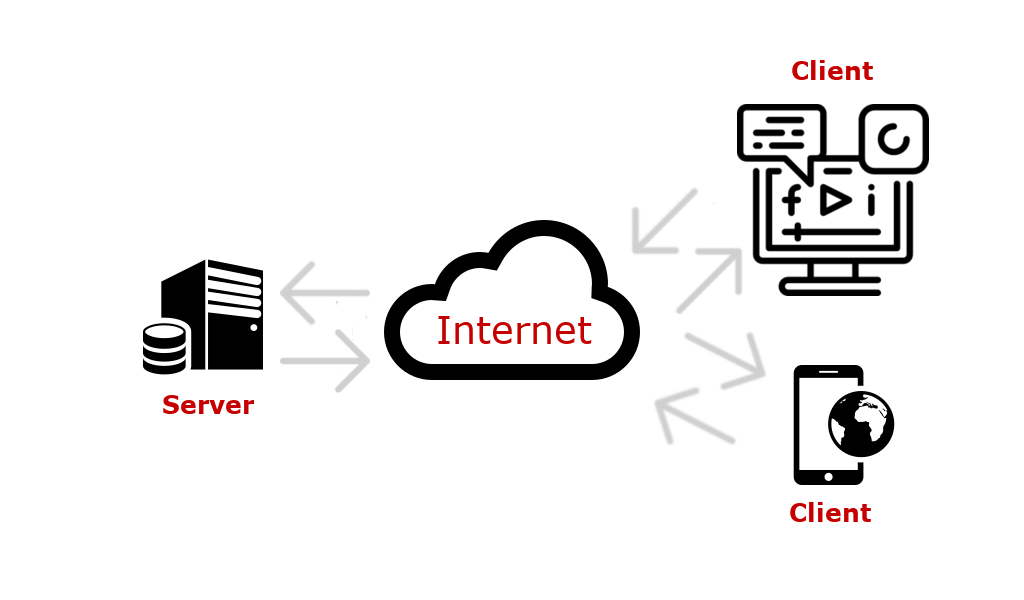
\includegraphics[width=1\textwidth]{client-server.png}
  \caption{Client-server architecture in the Internet.}
  \label{fig:client-server}
\end{figure}
\subsubsection{Multitier architecture}\index{Software!architecture!multitier}
Requesting resources for every asset sequentially and retrieving responses from the server usually is not enough in the current environment. Complex cloud solutions, modern mobile solutions and web applications\index{Web Application} contain a lot of logic. They should be optimized to improve maintainability and performance as well as to simplify development. In order to achieve scalable\index{Scalability} applications modular\index{Modularity} programming was introduced, in which each logical unit of the application is separated into individual modules. This is a foundation of multitier architecture\index{Software!architecture!multitier}. In that particular architecture application, data management and presentation tier are separated into
different tiers. Such architecture with different tiers is often present in applications are developed using modern architecture guidelines. An example of such logical division is presented by Figure \ref{fig:multitier_architecture}. The top tier is a presentation tier, it is responsible for showing the actual content for a user. Application tier contains business logic including authentication, security and other middleware\index{Middleware}. Persistent tier is a presentation tier for data. The bottom tier is optional and holds for example databases.
\begin{figure}[ht]
  \centering
      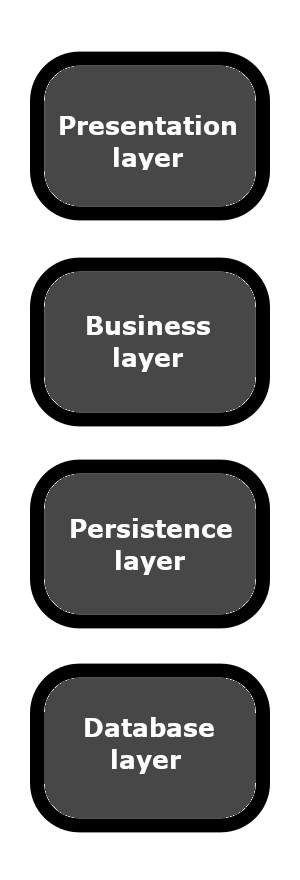
\includegraphics[width=0.2\textwidth]{layers.png}
  \caption{Multitier architecture\index{Software!architecture!multitier}, often present in modern applications.}
  \label{fig:multitier_architecture}
\end{figure}
\newpage
\subsubsection{Service-Oriented Architecture}\index{Software!architecture!Service-Oriented Architecture (SOA)}
Increasing technical needs from software development\index{Software!development} industry for more complex projects required more sophisticated architectures. SOA\index{Software!architecture!Service-Oriented Architecture (SOA)} helps to improve efficiency, scalability\index{Scalability} and management for large software projects \cite{bib:ibm_soa}. The idea behind SOA\index{Software!architecture!Service-Oriented Architecture (SOA)} is to divide logical parts into smaller chunks called components. Important fact is that each of them should be independent and limited as much as possible. In such a way changes in one of them should not influence other components. SOA\index{Software!architecture!Service-Oriented Architecture (SOA)} focuses on defining strategic goals, flexibility, providing business values and shared services with its inter-process communications between each other \cite{bib:soa_flexibility}. Typical implementations of SOA\index{Software!architecture!Service-Oriented Architecture (SOA)} often are performed using web services, e.g. REST\index{REpresentational State Transfer (REST)} and Simple Object Access Protocol (SOAP)\index{Simple Object Access Protocol (SOAP)}. This architecture style finds industrial application especially within enterprise-level applications, where the scope of the project is quite extensive. It helps the architecture to be more agile-oriented\index{Agile}, cost-effective and flexible.
\subsubsection{Model-View-Controller}\index{Software!architecture!Model-View-Controller (MVC)}
Architectural pattern designed for desktop applications, later adopted in many others environment such as the web and mobile applications is MVC\index{Software!architecture!Model-View-Controller (MVC)}. It has three core elements: Model, View and Controller. The first of them --- Model, contains business logic, handles application state, reads and writes data as well as validates data\index{Validation} on the front-end\index{Front-end} layer. The View, as its name suggests, presents certain views to the user based on data received from a controller. Its tasks includes the interaction with the user. The connection between model and views is provided by the Controller. This is a kind of a bridge between those two, as can be deduced from Figure \ref{fig:mvc}. The Controller can be understood as a managerial part of the application, as it interacts directly with both of the other elements of this architectural styles\index{Software!architecture}. The last one plays an important role, because the View and the Model should not know about each other; indirect communication between View and Model should be done through the Controller.\\
\newline
An obvious advantage of this architectural style\index{Software!architecture} is separation of content into different logical elements. Similar idea exists with the previously described multitier architecture\index{Software!architecture!multitier}. It helps to organize source code into different layers, by that cleaner code is easier to achieve. Maintenance of such application with its future extensions is also improved. Easier modifications, logical grouping, low coupling\footnote{Writing software in such a way that all classes work independently without relying on each other.}, simultaneous development or reusability are definitely positive sides of MVC\index{Software!architecture!Model-View-Controller (MVC)}. The view should not handle the business logic, because it is responsible just for showing the actual content. The model should focus solely on business logic, adding such methods to the controller will cause it to be overwhelmed after some time. The controller is a binder between these two.
\begin{figure}[ht]
  \centering
      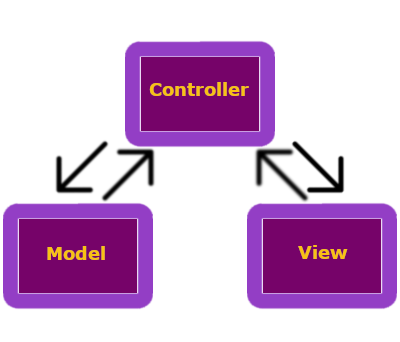
\includegraphics[width=0.5\textwidth]{mvc.png}
  \caption{MVC\index{Software!architecture!Model-View-Controller (MVC)} architectural style.}
  \label{fig:mvc}
\end{figure}
\subsubsection{Model-View-ViewModel}\index{Software!architecture!Model-View-ViewModel (MVVM)}
The MVVM\index{Software!architecture!Model-View-ViewModel (MVVM)} architecture is an important concept in terms of this research, since Angular\index{Angular} itself follows many of the MVVM\index{Software!architecture!Model-View-ViewModel (MVVM)} rules. The ViewModel main tasks include managing the model and transferring its data to the view. Simply speaking it is responsible for transforming the data to such format the view can present to the user in an acceptable structure. The view elements are also different. In MVC\index{Software!architecture!Model-View-Controller (MVC)} it is more passive, whilst in MVVM\index{Software!architecture!Model-View-ViewModel (MVVM)} it contains events and data binding\footnote{Establishing connection between the user's view and business logic implemented in a model.}. Views are not maintaining their states. For this task the ViewModel element is responsible to synchronize it with the view. Sometimes MVVM\index{Software!architecture!Model-View-ViewModel (MVVM)} is also known as Model-View-Binder, due to the reason that it contains a binder. It controls communication between the view and the ViewModel. The binder also helps the developer to follow certain rules. Only exposed properties can be accessed by the ViewModel. Thus, it disallows breaking a good practices in an architectural style\index{Software!architecture}. Figure \ref{fig:mvvm} shows MVVM\index{Software!architecture!Model-View-ViewModel (MVVM)} architecture with its basic idea.\\
\newline
Arguments for MVVM\index{Software!architecture!Model-View-ViewModel (MVVM)} include better separation of the view layer from rest of the application. It makes easier for people working on the presentation layer, i.e. UI\index{User Interface (UI)} and UX\index{User Experience (UX)} designers. Instead of dealing with the business logic they can focus on the user interface itself. This way, it is more convenient to work on multiple tasks simultaneously, because each element of the MVVM architecture style has clear separation of functionalities. Last, but not least a positive argument for introducing such separation is an improved testability of such application. This is especially helpful for teams working with BDD\index{Behavior-Driven Development (BDD)} and Test-Driven Development (TDD)\index{Test-Driven Development (TDD)} approach.\\
\newline
Criticism against MVVM includes unnecessary overcomplication for smaller projects, where the UI\index{User Interface (UI)} layer itself is not too complex. Apart from that, another argument is that in larger applications there exists a problem with managing those layers once the source code grows to an enormous size. Moreover, such big projects can have difficulties with substantial memory consumption, due to many data bindings in the application. Due to this reason a component-based architecture\index{Software!architecture!component-based} has been implemented in the Angular\index{Angular} framework\index{Framework}.
\begin{figure}[ht]
  \centering
      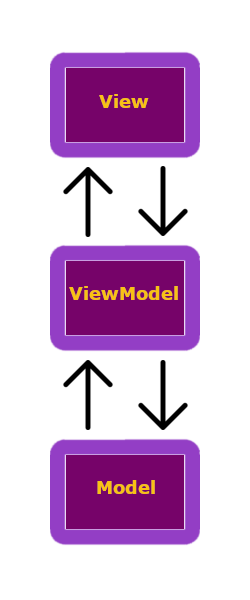
\includegraphics[width=0.3\textwidth]{mvvm.png}
  \caption{MVVM\index{Software!architecture!Model-View-ViewModel (MVVM)} architectural pattern.}
  \label{fig:mvvm}
\end{figure}
\subsubsection{Component-Based Architecture}\index{Software!architecture!component-based}
The architectural model implemented in Angular\index{Angular} is a component-based architecture\index{Software!architecture!component-based}. It has some similarities with others architectures described earlier. Components are a modular\index{Modularity}, portable\index{Portability} and reusable set of functionalities. This is an encapsulated entity of specific behaviours, styles and usually with one view to represent those.\\
\newline
The main focus is on component reusability, as it is shown on Figure \ref{fig:component-based}. Each logical part of an application is a separated component. However, defining one component should not collide with reusing it. In the following example a \textit{Call To Action (CTA) component} has been used twice. With the component-based architecture\index{Software!architecture!component-based} it is defined only once without code duplication. The application is instructed simply to show the same component twice, but in two different parts of the application. These reusable components reduces codebase, follows DRY\index{Don't Repeat Yourself (DRY)} principle and, ensures Separation of Concerns\index{Separation of Concerns (SoC)} (SoC).
\begin{figure}[ht]
  \centering
      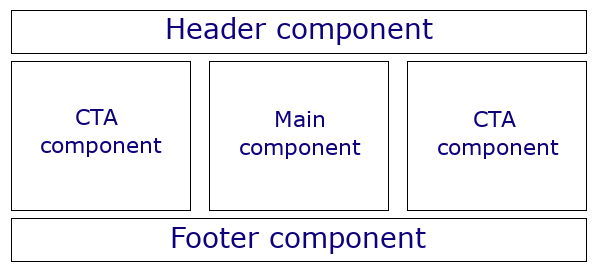
\includegraphics[width=1\textwidth]{component-based.png}
  \caption{Component-based architectural\index{Software!architecture!component-based} pattern.}
  \label{fig:component-based}
\end{figure}
\subsection{Software Security}
Cyber security\index{Cyber!security} is a relatively fresh part of IT. One of important parts in it is software security. This discipline is becoming more and more important. This is due to many reasons, i.e. big data leaks from companies such as Facebook \cite{bib:facebook_data_breach}, Marriott \cite{bib:marriott_data_breach}, Uber \cite{bib:uber_data_breach}, recent cryptocurrencies popularity \cite{bib:cryptocurrencies_hacking}, increasing cybercrime\index{Cybercrime} activity as well as introduction of General Data Protection Regulation (GDPR) \cite{bib:gdpr_eu} by European Union (EU). Tables \ref{tab:increase_statistics} and \ref{tab:numbers_statistics} show key statistics for cyber security\index{Cyber!security} market based on year 2017 \cite{bib:cyber_security_incidents}.
\begin{table}[ht]
\centering
    \begin{tabular}{ | l | c |}
    \hline
    \multicolumn{1}{|c|}{\textbf{Name of a security-related term}} & \multicolumn{1}{c|}{\textbf{Percentage [\%]}} \\ \hline
    Increase of attacks on Internet of Things (IoT) devices & 600 \\ \hline
    Annually growth of ransomware & 350 \\ \hline
    Companies keeping old sensitive files & 74 \\ \hline
    Users were never asked to change passwords & 65 \\ \hline
    China, as a source of attacks & 20 \\ \hline
    United States, as destination of attacks & 18 \\ \hline
    \end{tabular}
\caption{Percentage increase of cyber security\index{Cyber!security} incidents in 2017 in comparison to 2016.}
\label{tab:increase_statistics}
\end{table}
\begin{table}[ht]
\hspace*{-1cm}
\centering
    \begin{tabular}{ | l | c |}
    \hline
    \multicolumn{1}{|c|}{\textbf{Name of a security-related term}} & \multicolumn{1}{c|}{\textbf{Financial consequences [\$]}} \\ \hline
    Foreseen damage to hacking\index{Hacking}-related activities in 2021 & 6 trillions \\ \hline
    Average cost of cybercrime\index{Cybercrime} for financial services industry company & 18.3 millions \\ \hline
    Median cost of malware\index{Malware} attack on a company & 2.4 millions \\ \hline
    \end{tabular}
\caption{Costs of hacking\index{Hacking} activity.}
\label{tab:numbers_statistics}
\hspace*{-1cm}
\end{table}\\
Published in 2006, the book by Gary R. McGraw \cite{bib:building_security_in} was an eye opener to develop software in a secure manner. The author defines seven security touchpoints of secure software which is presented on Figure \ref{fig:security_touchpoints}. These points include: abuse cases, code review (tools), penetration\index{Software!testing!penetration} testing, risk analysis, risk-based security tests, security operations and security requirements. Although the book was published several years ago, from an architecture point of view the content remains valid, just the described tools may have changed. Hence, the ideas presented in the book will be the foundation for security requirements in this research project.
\begin{figure}[ht]
  \centering
      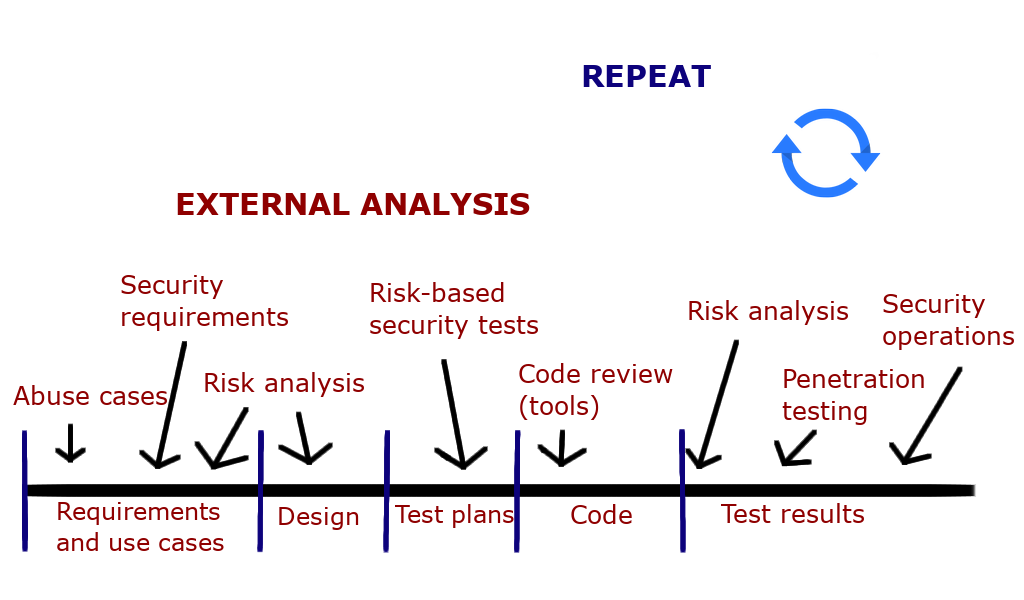
\includegraphics[width=1\textwidth]{touchpoints.png}
  \caption{Seven software security touchpoints \cite{bib:building_security_in}.}
  \label{fig:security_touchpoints}
\end{figure}\\
\newline
The security touchpoints are used depending by stage of the project, i.e. architecture and design, code, feedback from the field, requirements and use cases, test plans, tests and test results. Depending on the level of advancement different touchpoint should be used. For example, for test results firstly risk analysis should be used, then penetration\index{Software!testing!penetration} testing and finally security operations. When the software is already ready to be deployed --- in the final stage, it is more difficult to increase security. An extra touchpoint with added value could be analysis by an external team of security specialists, who have not contributed to the code. Often people not engaged in the project are able to find mistakes easier. The whole process should be repeatable, it can be seen as a beginning of software craftmanship\index{Software!craftmanship}.
\subsubsection{Risks}
Security of software is dependent on many factors, especially in the web where many logical layers exists. A structure of these layers can be represented in terms of the Internet Protocol Suite (TCP/IP)\index{Internet Protocol Suite (TCP/IP)}, as Figure \ref{tab:tcp_layers_protocols} shows. Different layers are managed by different protocols. This figure shows only a limited number of protocols, it is not an exhaustive list. Numbering layers in TCP/IP\index{Internet Protocol Suite (TCP/IP)} model starts from the bottom. Link layer in TCP\index{Transmission Control Protocol (TCP)} is the bottom one, while application layer is the top layer etc.
\begin{table}[ht]
\centering
    \begin{tabular}{ | c | l | l |}
    \hline
    \multicolumn{1}{|c|}{\textbf{Position}} & \multicolumn{1}{c|}{\textbf{TCP/IP\index{Internet Protocol Suite (TCP/IP)} layer name}} & \multicolumn{1}{c|}{\textbf{Typical protocols}} \\ \hline
    4. & Application & DNS\index{Domain Name System (DNS)}, FTP\index{File Transfer Protocol (FTP)}, HTTP\index{Hypertext Transfer Protocol (HTTP)}, HTTPS\index{Hypertext Transfer Protocol Secure (HTTPS)}, IMAP\index{Internet Message Access Protocol (IMAP)} \\ \hline
    3. & Transport & TCP\index{Transmission Control Protocol (TCP)}, UDP\index{User Datagram Protocol (UDP)} \\ \hline
    2. & Internet & ICMP\index{Internet Control Message Protocol (ICMP)}, IP\index{Internet Protocol (IP)} \\ \hline
    1. & Link & ARP\index{Address Resolution Protocol (ARP)}, Ethernet\index{Ethernet}, MAC\index{Medium Access Control (MAC)} \\ \hline
    \end{tabular}
\caption{Layers with its accordingly protocols in the TCP/IP\index{Internet Protocol Suite (TCP/IP)} model.}
\label{tab:tcp_layers_protocols}
\end{table}\\
Due to the reason the WWW has a very complicated structure, some kind of report to make developers aware about security was needed. Currently OWASP\index{The Open Web Application Security Project (OWASP)} provides insights of security for the web. Based on their cooperation with community, industry and researchers they are publishing every few years list of top ten security risks\index{Security!risks}. Recent lists are from 2013 \cite{bib:owasp_2013} and 2017 \cite{bib:owasp_2017}, presented by Figure \ref{tab:owasp_risks}. The order of the risks is according to their popularity, e.g. injection is the most popular type of security risk\index{Security!risks} for both reports.
\begin{table}[ht]
\hspace*{-1.75cm}
\centering
    \begin{tabular}{ | c | l | l |}
    \hline
    \multicolumn{1}{|c|}{\textbf{Position}} & \multicolumn{1}{c|}{\textbf{OWASP\index{The Open Web Application Security Project (OWASP)} Top 10 --- 2013}} & \multicolumn{1}{c|}{\textbf{OWASP\index{The Open Web Application Security Project (OWASP)} Top 10 --- 2017}} \\ \hline
    1. & Injection & Injection \\ \hline
    2. & Broken Authentication and Session Management & Broken Authentication \\ \hline
    3. & Cross-Site Scripting (XSS)\index{Cross-Site Scripting (XSS)} & Sensitive Data Exposure \\ \hline
    4. & Insecure Direct Object References & XML External Entities (XXE)\index{XML External Entities (XXE)} \\ \hline
    5. & Security Misconfiguration\index{Security!misconfiguration} & Broken Access Control \\ \hline
    6. & Sensitive Data Exposure & Security Misconfiguration\index{Security!misconfiguration} \\ \hline
    7. & Missing Function Level Access Control & XSS\index{Cross-Site Scripting (XSS)} \\ \hline
    8. & Cross-Site Request Forgery (CSRF)\index{Cross-Site Request Forgery (CSRF)} & Insecure Deserialization \\ \hline
    9. & Using Components with Known Vulnerabilities\index{Vulnerabilities!Known Vulnerabilities} & Using Components with Known Vulnerabilities\index{Vulnerabilities!Known Vulnerabilities} \\ \hline
    10. & Unvalidated\index{Validation} Redirects and Forwards & Insufficient Logging \& Monitoring \\ \hline
    \end{tabular}
\caption{Ten Most Critical Security Risks\index{Security!risks} in Web Applications\index{Web Application} in 2013 and 2017, by OWASP.}
\label{tab:owasp_risks}
\hspace*{-2.25cm}
\end{table}\\
One of the crucial elements in web security\index{Security!web} is associated with transferring data between web services. Web services are nowadays mostly based on the RESTful\index{REpresentational State Transfer (REST)!RESTful} architecture style. This architecture style is simple and flexible way to design Application Programming Interfaces (APIs)\index{Application Programming Interface (API)}, called RESTful\index{REpresentational State Transfer (REST)!RESTful} APIs\index{Application Programming Interface (API)}. REST\index{REpresentational State Transfer (REST)} takes advantage of existing protocols (HTTP\index{Hypertext Transfer Protocol (HTTP)}). Response objects are usually in JavaScript Object Notation (JSON)\index{JavaScript Object Notation (JSON)}, eXtensible Markup Language (XML)\index{eXtensible Markup Language (XML)}, YAML Ain't Markup Language (YAML)\index{YAML Ain't Markup Language (YAML)} or other text-based formats. This is an advantage over SOAP\index{Simple Object Access Protocol (SOAP)} which defines responses to be returned with a XML\index{eXtensible Markup Language (XML)} format. Even though SOAP\index{Simple Object Access Protocol (SOAP)} is an official web standard, REST\index{REpresentational State Transfer (REST)} is getting more popular. Its complexity is smaller, it provides higher performance and scales easier. SOAP\index{Simple Object Access Protocol (SOAP)} is a protocol, while REST\index{REpresentational State Transfer (REST)} is an architecture style. However, they both can be used for the same purpose and thus can be compared with each other. An example of the SOAP\index{Simple Object Access Protocol (SOAP)} is the PayPal SOAP\index{Simple Object Access Protocol (SOAP)} API\index{Application Programming Interface (API)} \cite{bib:soap_api}, while for the REST\index{REpresentational State Transfer (REST)} it is WordPress\index{WordPress} REST\index{REpresentational State Transfer (REST)} API\index{Application Programming Interface (API)} \cite{bib:wordpress_api}. The reason for REST's popularity might be its simplicity in comparison to SOAP\index{Simple Object Access Protocol (SOAP)}, but it comes with the price of security. SOAP\index{Simple Object Access Protocol (SOAP)} comes with standardized security rules such as built-in Atomicity, Consistency, Isolation, Durability (ACID)\index{Atomicity, Consistency, Isolation, Durability (ACID) compliance} compliance or authorization provides higher level of security using when implementing its guidelines called \textit{WS-Security}. Due to them SOAP\index{Simple Object Access Protocol (SOAP)} enables security implementation in more standardized way. REST\index{REpresentational State Transfer (REST)} supports JSON\index{JavaScript Object Notation (JSON)} parsing which is usually faster than parsing XML\index{eXtensible Markup Language (XML)} \cite{bib:parsing}. This is one of the most valuable advantages over SOAP\index{Simple Object Access Protocol (SOAP)} and could be one of the reasons why it is more popular than SOAP\index{Simple Object Access Protocol (SOAP)}. Especially given the popularity of mobile devices, as for those end user every second matters. However, in enterprise-level web services which require higher security, e.g. financial services or in telecommunication companies, SOAP\index{Simple Object Access Protocol (SOAP)} is still the preferred way for data communication.\\
\newline
The progressive popularity of mobile and web applications\index{Web Application}, mostly based on REST\index{REpresentational State Transfer (REST)}, enforced OWASP\index{The Open Web Application Security Project (OWASP)} to prepare special requirements for software which uses REST as a method to communicate between web services. The good security practices recommended by OWASP\index{The Open Web Application Security Project (OWASP)} \cite{bib:owasp_rest_security} include:
\begin{itemize}
    \item Access control --- access control has to be enforced in all micro services which is a bit more complicated in comparison to monolithic applications.
    \item API keys\index{Application Programming Interface (API)!key} --- to protect endpoints API keys\index{Application Programming Interface (API)!key} should be used.
    \item Audit logs --- analysis of token validation\index{Validation} errors with security alerts are helpful to detect attacks.
    \item Cross-Origin Resource Sharing (CORS)\index{Cross-Origin Resource Sharing (CORS)} --- a mechanism which allows website at specific domain to have permissions to access some resources from a different domain.
    \item Error handling\index{Error Handling} --- error message can be a source of potential helpful information for an attacker, thus revealing technical details about them is a security mistake.
    \item HTTP\index{Hypertext Transfer Protocol (HTTP)!header} return codes --- semantic status codes should be used for responses in order to follow proper HTTP\index{Hypertext Transfer Protocol (HTTP)} specification for different scenarios.
    \item HTTPS\index{Hypertext Transfer Protocol Secure (HTTPS)} --- each API\index{Application Programming Interface (API)} endpoint must provide HTTPS\index{Hypertext Transfer Protocol Secure (HTTPS)} to protect authentication data such as API keys\index{Application Programming Interface (API)!key} or user credentials.
    \item Input validation\index{Validation!input} --- by default untrusting input parameters is a good practice, thus entered data should be validated\index{Validation}. Only strictly allowed can proceed further, suspicious input must be rejected. 
    \item JSON Web Tokens (JWT)\index{JavaScript Object Notation (JSON)!JSON Web Tokens (JWT)} --- protection using digital signatures\footnote{Called also cryptographical\index{Cryptography} signatures, those are mathematical methods to verify authenticity of a certain message.} or by Message Authentication Code (MAC) is required to protect this standard, because they are often used for security tokens.
    \item Management endpoints --- strong protection must be delivered by Access Control List (ACL) or firewall rules\index{Firewall!rules}. When accessing online multi-factor they should be hided from the Internet.
    \item Restrict HTTP\index{Hypertext Transfer Protocol (HTTP)!header} methods --- rejecting all HTTP\index{Hypertext Transfer Protocol (HTTP)!header} methods that are not on the white list with a response code 405, i.e. \textit{Method Not Allowed}.
    \item Security headers\index{Security!header} --- returning \textit{Content-Type} header with \textit{charset} causes correct interpretation of the content by the browser and the server's correct answer also is important against XSS\index{Cross-Site Scripting (XSS)}.
    \item Sensitive information in HTTP requests\index{Hypertext Transfer Protocol (HTTP)!request} --- to avoid leakage of secret API keys\index{Application Programming Interface (API)!key}, credentials or security tokens cannot be shown in the URL. Instead, GET\index{Hypertext Transfer Protocol (HTTP)!GET request}, POST\index{Hypertext Transfer Protocol (HTTP)!POST request} and PUT\index{Hypertext Transfer Protocol (HTTP)!PUT request} methods should handle it in their appropriate sections to keep sensitive data.
    \item Validate\index{Validation} content types --- validating\index{Validation} incoming requests and sending safe responses with appropriate content types are required for correct interpretation on the client-side.
\end{itemize}
There are many security risks\index{Security!risks} on different layers which can cause to defeat security defenses. Thus, in the software industry information about many threats\index{Threat} can be heard. These mostly has been caused by exploiting vulnerabilities\index{Vulnerabilities}. Often, even one weakness in the application was enough to break it totally or cause a data breach\index{Data Breach}. As the list shows, there are many parts to take care of.
\subsubsection{Vulnerabilities}\index{Vulnerabilities}
General issues related to security are based on \textit{vulnerabilities}\index{Vulnerabilities} --- possible weaknesses in a software which can be exploited by an attacker \cite{bib:vulnerability_fsecure}. They should be distinguished from security risks\index{Security!risks}, those two are different terms. Currently many applications are based on cloud solutions, available through different types of services. These includes Infrastructure as a Service (IaaS)\index{Infrastructure as a Service (IaaS)}, Platform as a Service (PaaS)\index{Platform as a Service (PaaS)} or Software as a Service (SaaS)\index{Software as a Service (SaaS)}. Vulnerabilities\index{Vulnerabilities} can occur on many different layers. Beginning from web application\index{Web Application} core source code, through network-related problem, all way to cryptographical\index{Cryptography} methods. Such complicated combination of layers in a typical web-based project leads to many possible weaknesses. They are caused by lack of testing, obsolete encryption algorithms, poor storage management, programming mistakes, unencrypted communication protocols traffic, usage of APIs\index{Application Programming Interface (API)} with malicious code, weak passwords, wrong databases configuration \cite{bib:cloud_vulnerabilities}. Monitoring of Common Vulnerabilities and Exposures (CVE)\index{Common Vulnerabilities and Exposures (CVE)} is a valuable source of potential security risks\index{Security!risks}. Lists of those are published by National Institute of Standards and Technology (NIST) \cite{bib:nist_list}. The records are based on specially designed for it website \cite{bib:cve_website} which is kept up-to-date by the community and security researchers. From developers perspective it is important not to use dependencies\index{Dependencies} and software versions which contains any kind of weaknesses. Automatic monitoring as well as updating them as fast as possible once security updates are deployed is a typical countermeasure\index{Countermeasures}.
\subsubsection{Threats}\index{Threat}
A danger with possible harmful to certain system complications due to intentional or accidental activity is called a \textit{threat}\index{Threat} \cite{bib:thomas}. Effects of a successful hacking\index{Hacking} activity can compromise availability, confidentiality or integrity. Typical threats\index{Threat} are botnets\index{Botnet}, computer worms, fake security software, malicious spyware\index{Spyware}, malware\index{Malware}, phishing\index{Phishing}, rootkits\index{Rootkit}, spam\index{Spam}, Trojan horses\index{Trojan horse} and viruses\index{Virus}. Most of them target machines, but some of them humans. Machines usually respond automatically, thus their security relies on the software which is supposed to defend from malicious activity. Humans should follow security policies, have basic knowledge or at least installed antivirus software with up-to-date virus\index{Virus} definitions database.
\subsubsection{Control}
Assurance of security requires that developers follow certain rules and should be controlled through earlier established standards. Comprehensive list of preventive measures has been published by OWASP\index{The Open Web Application Security Project (OWASP)} in 2018 \cite{bib:owasp_controls} and includes:
\begin{enumerate}
    \item Define security requirements.
    \item Leverage security frameworks\index{Framework} and libraries.
    \item Secure database access.
    \item Encode and escape data.
    \item Validate all inputs\index{Validation!input}.
    \item Implement digital identity.
    \item Enforce access controls.
    \item Protect data everywhere.
    \item Implement security logging and monitoring.
    \item Handle all errors and exceptions.
\end{enumerate}
These rules are easy to follow not only on the stage of development, but also during validation\index{Validation}, i.e. when assessing how secure the application is. Web applications\index{Web Application} contains many layers of source code present in business logic, controllers, databases, views etc. That is why ensuring high level on security includes to meet the requirements on all those layers. Modern security defenses have many layers of security. It means that breaking into one layer does not mean the whole system is broken. Keeping security in mind is easier with these guidelines, from security analysis\index{Security!analysis} point of view as well as software development\index{Software!development}.
\subsubsection{Secure Software Development Life Cycle}
High quality source code with agile-oriented\index{Agile} way of working is called SDLC\index{Software Development Life Cycle (SDLC)}. This is presented on Figure \ref{fig:sdlc}. Its first stage starts with planning requirements for the project, followed by defining requirements, designing the product architecture, developing, testing and deploying the product. It can be easily implemented into Agile\index{Agile} methodology, which will render the SDLC\index{Software Development Life Cycle (SDLC)} to become iterative.
\begin{figure}[ht]
  \centering
      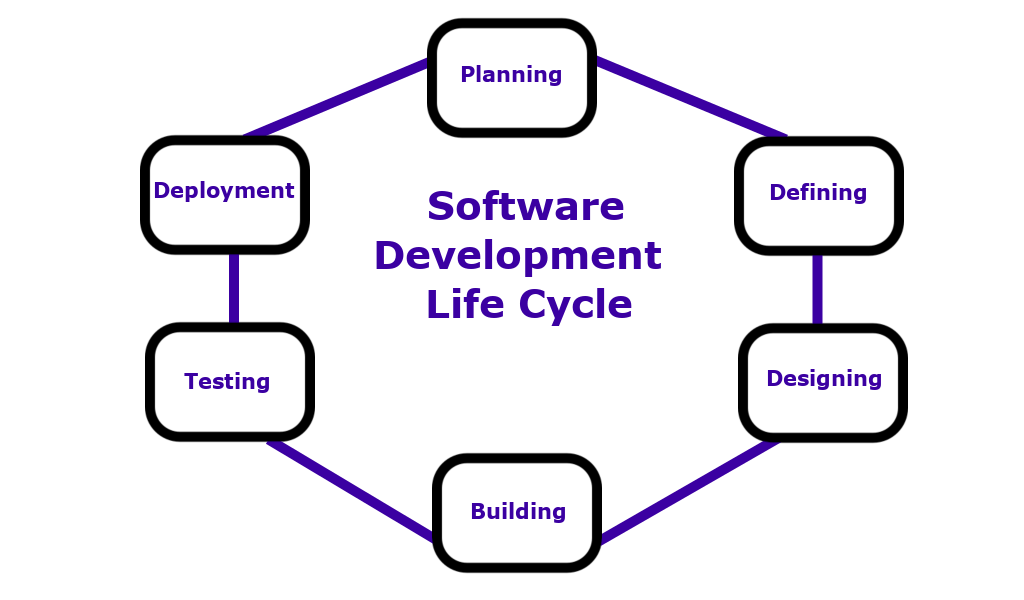
\includegraphics[width=0.7\textwidth]{sdlc.png}
  \caption{SDLC\index{Software Development Life Cycle (SDLC)} methodology.}
  \label{fig:sdlc}
\end{figure}\\
\newline
On top of the framework\index{Framework} designed for security requirements a new model has been proposed called SSDLC\index{Secure Software Development Life Cycle (SSDLC)}. Its basic concept is presented by Figure \ref{fig:ssdlc}. Difference between those two models by naming includes the first two stages, where in SSDLC\index{Secure Software Development Life Cycle (SSDLC)} security is mentioned with a priority. The security definition phase would include planning as well. The research phase would define general concept of that application. However, even though the next phases look exactly the same, their tasks will be slightly different. With more focus on security, e.g. for testing apart functional tests, fuzzing\footnote{Providing invalid, random and unexpected inputs.}\index{Fuzzing} or mutation testing\footnote{Changing (mutating) statements in a source code and observe if there are any errors.}\index{Software!testing!mutation} could be added. Similarly to the SDLC\index{Software Development Life Cycle (SDLC)}, its extension called SSDLC\index{Secure Software Development Life Cycle (SSDLC)} can be smoothly implemented into teams working in Agile\index{Agile}, making it an iterative process.
\begin{figure}[ht]
  \centering
      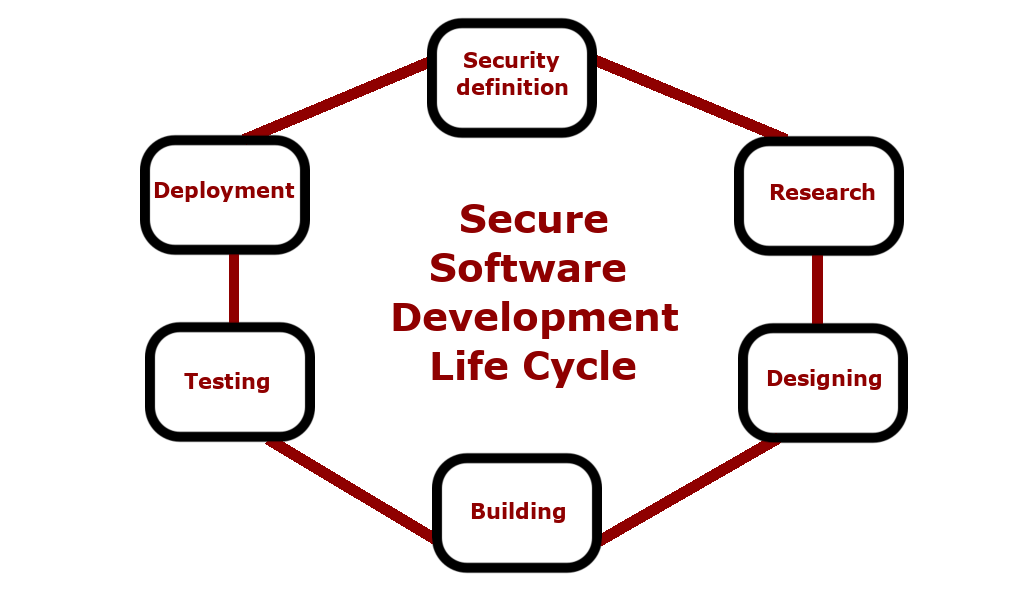
\includegraphics[width=0.7\textwidth]{ssdlc.png}
  \caption{SSDLC\index{Secure Software Development Life Cycle (SSDLC)} methodology.}
  \label{fig:ssdlc}
\end{figure}\\
\newline
\subsubsection{SecDevOps\index{SecDevOps}}
Prioritizing security on the first position in DevOps\index{DevOps} projects is getting called SecDevOps\index{SecDevOps}. Apart this, there are DevSecOps\index{DevSecOps} (Development, Security and Operations) and DevOpsSec\index{DevOpsSec} (Development, Operations and Security).\\
\newline
The main difference between these three terms, i.e. SecDevOps\index{SecDevOps}, DevSecOps\index{DevSecOps} and DevOpsSec\index{DevOpsSec} is the \textit{Sec} part. In terms of security this is crucial, because it defines on which stage of the SDLC\index{Software Development Life Cycle (SDLC)} it should be placed. For SSDLC\index{Secure Software Development Life Cycle (SSDLC)} the correct way supposed to be only SecDevOps\index{SecDevOps}. In terms of the SecDevOps security is defined already on the earliest stage of a project. The DevSecOps predicts security checks after development. DevOpsSec will take security into considerations once the application will be deployed.\\
\newline
Improving security\index{Security!improving} in the last part of product development might be difficult to achieve. The reason for that is when all the programming is already done and deployed as designed, changes for security reasons would need to imply changes on the architecture level. Enterprise-level applications might be very difficult to change on that level, sometimes it is even impossible to fully integrate security, as it should be. In a positive scenario it would take significant amount of time to make it properly. However, it is supposed to be the easiest solution. The currently popular DevOps\index{DevOps} technique is present in many companies delivering modern applications. In these projects which have started before SecDevOps\index{SecDevOps} was born it is kind of natural way to extend it like so and thus follow DevOpsSec.\\
\newline
DevSecOps\index{DevSecOps} makes security a higher priority than DevOpsSec\index{DevOpsSec}. In that model it is placed directly after implementation, before deployment. In terms of security it is a more correct approach, because the application is not delivered to the commercial environment before passing necessary security tests. This approach causes similar problems. Once security flaws will be discovered, then sometimes it might be quite difficult to increase security without changing the architecture significantly. However, in terms of security this is much better approach.\\
\newline
Including code reviews, proper cryptography\index{Cryptography} usage, defensive techniques based on OWASP\index{The Open Web Application Security Project (OWASP)} guidelines, programming best practices\index{Programming Best Practices}, secure access control, static code analysis\index{Static Code Analysis}, threat\index{Threat} modeling, vulnerability\index{Vulnerabilities} assessment and others security-related mechanisms at the starting stage of an IT project is what SecDevOps\index{SecDevOps} is about. In this technique security requirements are defined before development starts The problem of completely redesigning the architecture due to security changes does not exist, because it is defined during first stage of the project. Only new vulnerabilities\index{Vulnerabilities} have to be taken into consideration, but with security first approach\index{Security!first approach} it is easier to manage source code, than vice versa. It might come with a cost of slower development. However, in a long term period decreasing potential of security issues results in a smaller amount of successful attacks. They become more and more expensive once getting older.
\newpage
\huge Chapter 3
\section{Single-Page Applications}
\normalsize The traditional way to build web applications\index{Web Application} is based on a MPA\index{Multi-page applications (MPA)} approach. In the MPA for any action page is loaded. A different approach is taken by SPA, where the client loads all the resources during first load only. Therefore, it does not need page reloads during events such as clicks, routing\index{Routing}, sending forms etc. Even if the browser is closed, then due to cache mechanism it loads fast for the second time and later on. By that it provides better UX\index{User Experience (UX)} for the client-side. Currently many modern web applications follow the SPA\index{Single-Page Application (SPA)} model.
\subsection{Web Applications\index{Web Application}}
Typical layer separation for web applications is done by separating the front-end\index{Front-end} layer --- presented in a browser, the back-end\index{Back-end} layer --- handled by a web server\index{Web Server} and the database layer. Figure \ref{fig:web_application_layers} clearly shows relationship between those three. The browser is responsible for displaying the content to the user. The server handles requests from the front-end\index{Front-end} layer and sends responses back to the browser. The database layer stores data which may include user credentials hashed values. SPAs\index{Single-Page Application (SPA)} are naturally also considered to be web applications. They are placed on the browser side, however due to their specification they are able to provide a rich front-end\index{Front-end} experience. In the JavaScript\index{JavaScript} world typical technological stacks on the front-end\index{Front-end} side includes Angular\index{Angular}, React\index{React} or Vue.js\index{Vue.js}. The server layer can be implemented by Node.js\index{Node.js} with Express\index{Express}. MongoDB\index{MongoDB} is an example of natural database for the JavaScript\index{JavaScript} stack. However, the back-end\index{Back-end} could be also any different technology, e.g. C\#\index{C\#}, Go\index{Go}, Java\index{Java}, Ruby on Rails\index{Ruby on Rails} etc. The JavaScript\index{JavaScript}-related technologies plays nicely together, but any other back-end\index{Back-end} and database could be used as well.
\begin{figure}[ht]
  \centering
      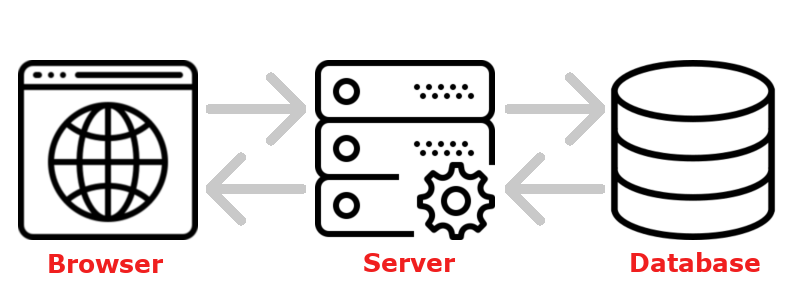
\includegraphics[width=0.7\textwidth]{web_applications.png}
  \caption{Logical layers separation of a typical web application\index{Web Application}.}
  \label{fig:web_application_layers}
\end{figure}
\subsubsection{JavaScript\index{JavaScript}}
In 1995 the programming language JavaScript\index{JavaScript} originally was introduced to improve interaction on the client-side of web application in a browser. Over many years it changed significantly. Currently is the most frequently used language in the world, as can be seen on Figure \ref{fig:stack_overflow_report}. Not only the front-end\index{Front-end} layer is currently a domain of JavaScript\index{JavaScript}, but it can also be found on the server-side (Node.js\index{Node.js}). Building full stack web applications\index{Web Application} can be done using MongoDB\index{MongoDB}, Express\index{Express}, Angular\index{Angular} and Node.js\index{Node.js} (MEAN) stack\index{MongoDB, Express, Angular, Node.js (MEAN) stack}. Other use cases includes: cross-platform solutions (Electron, Meteor), mobile applications (Apache Cordova\index{Apache!Cordova}, Ionic\index{Ionic}), Progressive Web Applications\index{Progressive Web Application (PWA)}\footnote{Web applications\index{Web Application} with access to mobile native applications functionalities.} (PWA\index{Progressive Web Application (PWA)}) or even IoT (IoT.js).
\begin{figure}[ht]
\centering
\begin{tikzpicture}[x={(.1,0)}]
\foreach  \l/\x/\c[count=\y] in {
Ruby\index{Ruby}/10.1,
TypeScript\index{TypeScript}/17.4,
C\index{C}/23.0,
C++\index{C++}/25.4,
PHP\index{PHP}/30.7,
C\#\index{C\#}/34.4,
Python\index{Python}/38.8,
Bash\index{Bash}/39.8,
Java\index{Java}/45.3,
SQL\index{Structured Query Language (SQL)}/57.0,
CSS\index{Cascading Style Sheets (CSS)}/65.1,
HTML\index{HyperText Markup Language (HTML)}/68.5,
JavaScript\index{JavaScript}/69.8
}
{\node[left] at (0,\y) {\l};
\fill[\c] (0,\y-.02) rectangle (\x,\y+.02);
\node[right] at (\x, \y) {\x\%};}
\draw (0,0) -- (100,0);
\foreach \x in {0, 10, ..., 100}
{\draw (\x,.2) -- (\x,0) node[below] {\x\%};}
\draw (0,0) -- (0,13);
\end{tikzpicture}
\caption{Most popular technologies, annual report by Stack Overflow for 2018 \cite{bib:stack_overflow_report}. Includes languages with at least 10\% usage by software developers.}
\label{fig:stack_overflow_report}
\end{figure}\\
JavaScript\index{JavaScript} is a high-level, interpreted language which complies with ECMAScript\index{ECMAScript} --- a scripting-language specification on which JavaScript\index{JavaScript} is based. Basic features of this language include: delegation, dynamically typed, functional, object-based, supports structured programming and wide usage of prototypes. For a long time it has been considered as a non-secure programming language due to its unsafe nature. However, its recent popularity also led to interest in the topic of security in this certain technology. Combination of Document Object Model (DOM)\index{Document Object Model (DOM)} with its manipulation by JavaScript\index{JavaScript} are potential source of vulnerabilities\index{Vulnerabilities}. Possible attacks are CSRF\index{Cross-Site Request Forgery (CSRF)}, XSS\index{Cross-Site Scripting (XSS)} or other client-based possible exploits. However, this is not limited only to the front-end\index{Front-end} layer of web applications\index{Web Application}. As mentioned previously, JavaScript\index{JavaScript} has been applied in different environments. Hence, its security becomes more and more important. Especially when handling authentication, authorization, sensitive data or payments in the business logic layer.\\
\newline
Its ecosystem changed significantly over past several years. Currently plain JavaScript\index{JavaScript} (without any frameworks\index{Framework} or libraries, also known as \textit{Vanilla JS}) is not often used in developing modern applications. Frameworks\index{Framework} such as Angular\index{Angular}, React\index{React} and Vue.js\index{Vue.js} or libraries like jQuery\index{jQuery}, RxJS\index{RxJS} and Underscore.js\index{Underscore.js} are daily used by hundreds of thousands of developers. Moreover, workflow for this specific language includes its specific tools, such as Babel, Bower, ESLint, Grunt, Gulp, Karma, npm, webpack\index{webpack}, Yarn, Yeoman etc. They automate certain tasks, bundle source code for deployment, check syntax, transpile\index{Transpilation} into a syntax readable by the browser and takes care of many other processes.
\subsubsection{TypeScript\index{TypeScript}}
Angular\index{Angular} is built in TypeScript\index{TypeScript}, a programming language introduced by Microsoft in 2012. TypeScript\index{TypeScript} is recognized and advertised as a superset of JavaScript\index{JavaScript}. As its name suggests --- it is strongly typed language. Apart strong typing other features includes asynchronous pattern, classes, enumerations, generics, interfaces, namespaces, modules, tuples\index{Tuple}, typed annotations and typed inferences. Angular\index{Angular} applications projects source code is written in TypeScript\index{TypeScript} and transcompiled to JavaScript\index{JavaScript}. Such kind of technique provides a way to execute written code by a browser. It will be the main programming language used to develop the practical side of this research project. However, once the application is deployed JavaScript\index{JavaScript} is the language present in the browser responsible for executing it properly. TypeScript\index{TypeScript} is not natively supported by the browsers, at least at this time of writing this thesis.
\subsection{Frameworks}\index{Framework}
Often modern web applications\index{Web Application} are taking advantage of using frameworks\index{Framework}, external libraries or both. Frameworks\index{Framework} defines the structure of an application. Libraries provide ready functions to be used by the developer, without the need to work in a plain language, e.g. Vanilla JS. Nowadays, developers communities mostly use frameworks\index{Framework} such as Angular\index{Angular}, React\index{React} or Vue.js\index{Vue.js} on the front-end\index{Front-end}. Frameworks\index{Framework} are important additions to programming languages because they motivate on developers to follow certain rules. Using them, projects are easier to follow and maintenance becomes simpler as such application have a more structured architecture. Efficient and scalable SPAs\index{Single-Page Application (SPA)} are usually based on such frameworks\index{Framework}. In this thesis, Angular\index{Angular} is studied. Its environment is mature, provides many best practices, good technical documentations, as well many problems (including security) has been solved since that time Google introduced it in 2016. The Angular\index{Angular} framework\index{Framework} should not be mistaken for AngularJS\index{AngularJS} framework\index{Framework}, which was introduced by Google in 2010 but in fact is a completely framework with a completely different approach solving different problems.
\subsection{Angular}
One of the most popular frameworks\index{Framework} for developing SPAs\index{Single-Page Application (SPA)} is currently Angular\index{Angular}. It is not only possible to use Angular\index{Angular} for web applications\index{Web Application}, but with its cross platform approach Angular\index{Angular} can also be used to create desktop and mobile applications. AngularJS\index{AngularJS} follows the MVC\index{Software!architecture!Model-View-Controller (MVC)} architectural pattern, but Angular\index{Angular} does not. Moreover, it also does not follow MVVM\index{Software!architecture!Model-View-ViewModel (MVVM)}, but takes many practices from it. Instead, Angular\index{Angular} follows a component-based architecture\index{Software!architecture!component-based}. Angular\index{Angular} consists the component itself, its View and business logic. Such components must be added to declarations in a parent module, then assigned to the View, i.e. \textit{.html} file and is rendered by the browser.\\
\newline
Angular\index{Angular} provides many built-in features, e.g. animations, code optimization techniques like Ahead-of-Time\footnote{Compilation process to produce efficient JavaScript\index{JavaScript} source code during build time to speed up rendering in the browser.} (AoT)\index{Ahead-of-Time (AoT)} or lazy loading\footnote{Approach to defer loaded content to the moment when it is actually needed, instead of loading them upfront.}, dependency injection\footnote{Technique for producing loosely coupled code with supplying dependencies\index{Dependencies} to another object.}, form validation\index{Validation}, internationalization, offline capabilities, security mechanisms, simplified HTTP\index{Hypertext Transfer Protocol (HTTP)} API\index{Application Programming Interface (API)} and type safety (TypeScript\index{TypeScript}). Thus, it is a good choice for scalable applications, even though it has its specific workflow. At the beginning this workflow can be seen as a disadvantage over other frameworks\index{Framework}, but such kind of mature ecosystem is incredibly important when releasing stable software. There is no need to rely on third-party packages, because the core functionalities provided by Google are already forming ripe environment to create wide spectrum of web applications\index{Web Application}. It is still possible to extend working environment by using one of thousands of extensions developed by the community. It clearly shows how popular Angular\index{Angular} is.\\
Newly introduced mechanisms such as Angular\index{Angular} Ivy\footnote{Rendering engine responsible for providing smaller bundles faster.}, i18n\footnote{Internationalization capabilities.}, tree shaking\footnote{Dead-code elimination.} are definitely interesting. However, even more helpful changes for developers are coming. One example is adding to the Angular CLI\index{Angular!Command Line Interface (CLI)} default renderer based on the Angular Ivy\index{Angular!Ivy} engine. This clearly shows Angular's\index{Angular} potential. Google keeps, apart from having an internal, dedicated team for Angular\index{Angular} improvements this framework\index{Framework} open source. This helps the community to contribute with their ideas to further improve it. One of successful ideas coming from the community includes introduction of NgRx\index{NgRx}, a reactive state management inspired by Redux\footnote{JavaScript\index{JavaScript} library for managing application state.}.\\
\newline
Another reason to create a SPA\index{Single-Page Application (SPA)} based on Angular\index{Angular} is its willingness to test wide spectrum of SPA\index{Single-Page Application (SPA)} features. These could be potential source of security vulnerabilities\index{Vulnerabilities}. Hence, more features, such as accessibility or offline capabilities can be integrated using the latest version of Angular\index{Angular} and validated\index{Validation} how secure the application is.
\subsubsection{Security}
There are several best practices for security in Angular\index{Angular} applications such as using the latest version of this framework\index{Framework}, do not make any direct modifications to the core of Angular\index{Angular} and avoid usage of flagged as a security risk\index{Security!risks} APIs\index{Application Programming Interface (API)}. However, security on the front-end\index{Front-end} layer is more than that. Terms such as Content Security Policy (CSP)\index{Content Security Policy (CSP)}, CORS\index{Cross-Origin Resource Sharing (CORS)}, CSRF\index{Cross-Site Request Forgery (CSRF)}, Cross-Site Script Inclusion (XSSI)\index{Cross-Site Script Inclusion (XSSI)}, data sanitization or XSS\index{Cross-Site Scripting (XSS)} are one of possible vulnerabilities\index{Vulnerabilities} developers can face.\\
\newline
XSS\index{Cross-Site Scripting (XSS)} is an attack, in which malicious code can be injected into an application. Prevention includes defending the DOM\index{Document Object Model (DOM)} from ability to insert attacker's code there, e.g. using a \textit{script} tag. By default Angular\index{Angular} classifies all values as untrusted, while inserted values via DOM\index{Document Object Model (DOM)} are sanitized. That way, suspicious values are escaped by its framework\index{Framework} design. Apart from possible client-side XSS\index{Cross-Site Scripting (XSS)} attacks, there also exists server-side XSS\index{Cross-Site Scripting (XSS)}. For these different type of protection should be ensured. For that reason generating Angular\index{Angular} templates on the back-end\index{Back-end} layer by using templating languages can be a source of unconscious template-injection vulnerabilities\index{Vulnerabilities}. In terms of security it is better to use automated escaping of values provided by templating language itself, but not by generated Angular\index{Angular} templates based on it.\\
\newline
The security model for XSS\index{Cross-Site Scripting (XSS)} includes also using an offline template compiler to avoid template injection. This technique also improves performance. Dynamically generated templates based on concatenation of user input and templates are not considered to be secure. They bypass built-in security protection of Angular\index{Angular}.\\
\newline
Data sanitization is one of methods to prevent XSS\index{Cross-Site Scripting (XSS)} attacks. It is performed to filter untrusted values from source code. Angular\index{Angular} recognizes six security contexts, i.e. HTML\index{HyperText Markup Language (HTML)}, none, resource URL, script, styles and URL. An important note is that resource URL is not sanitized by Angular\index{Angular}, because it is simply not doable. Sometimes developers have to access DOM\index{Document Object Model (DOM)} APIs\index{Application Programming Interface (API)} directly which is not recommended in terms of security. Hence, in that scenario built-in sanitization methods should be used, i.e. \textit{sanitize} of the \textit{DomSanitizer\footnote{Security helper for XSS\index{Cross-Site Scripting (XSS)} prevention when sanitizing values to be used in different DOM\index{Document Object Model (DOM)} contexts.}} with adequate security context. This technique is crucial, because native DOM\index{Document Object Model (DOM)} APIs\index{Application Programming Interface (API)} by default do not provide protection against security vulnerabilities\index{Vulnerabilities}. Therefore, manipulating DOM\index{Document Object Model (DOM)} via \textit{Renderer2}\footnote{Abstraction for manipulating DOM\index{Document Object Model (DOM)} without directly accessing it.}, instead of using \textit{ElementRef\footnote{Wrapper around native DOM\index{Document Object Model (DOM)} element.}} is considered to be more safe. Dependencies\index{Dependencies} are key elements when developing SPAs. Third-party APIs\index{Application Programming Interface (API)} might have calls to unsafe methods such as \textit{ElementRef}. Developers could assume that unit testing\index{Software!testing!unit} will provide clean code\index{Clean code} and it is all in terms of security. However, those are isolated\index{Isolation} tests which do not touch external dependencies\index{Dependencies} the community has to rely on. Hence, this is another reason to analyse security in Angular\index{Angular} in more depth before deployment.\\
\newline
Next protection against XSS\index{Cross-Site Scripting (XSS)} attacks is to introduce CSP into an application by permitting only allowed origins to be executed. Let consider an example, an URL \textit{https://my-trusted-source.com} is whitelisted by a web application\index{Web Application} \textit{https://myapp.com}, thus considered safe. That is why execution of scripts from \textit{https://my-trusted-source.com} on \textit{https://myapp.com} is permitted. On the other side, there exists a harmful sample script from \textit{https://malicious-code.com}. It has been not whitelisted by the \textit{https://myapp.com}. Therefore, \textit{https://malicious-code.com} cannot execute its scripts on \textit{https://myapp.com}. Defenses against XSS\index{Cross-Site Scripting (XSS)} in terms of CSP\index{Content Security Policy (CSP)} include the previously mentioned source whitelists. It is achieved using CSP\index{Content Security Policy (CSP)}-defined set of policy directives (e.g. \textit{default-src}, \textit{style-src}, \textit{script-src}, etc.) with whitelisted URLs \cite{bib:csp_reference}.\\
\newline
Apart from that, good programming practices have a positive impact on security as well. The first one is to disable executing \textit{eval()\footnote{Method for evaluation or executing an expression.}} and minimize inline codes. It might lead to detrimental behaviour of web application\index{Web Application}. These introduces the risk of DOM-based XSS\footnote{Modifying DOM\index{Document Object Model (DOM)} environment by executing scripts in victim's browser using client-side script.} vulnerability\index{Vulnerabilities} due to unsanitised values. That is another reason to use separated \textit{.js} files. Usage of \textit{eval()} seems to be outdated, however there are different object used in JavaScript\index{JavaScript} through which text can be injected, i.e. \textit{new Function()\footnote{Built-in constructor for defining a method.}}, \textit{setInterval()\footnote{Method for calling certain logic at specified interval.}} or \textit{setTimeout()\footnote{Method for evaluating an expression after specific number of milliseconds.}}. Potentially, this could end up with injection of malicious content. Thus, CSP\index{Content Security Policy (CSP)} by default blocks Strings in these functions and calls for these three methods should be written as inline functions rather than Strings \cite{bib:csp_google}. Information about security on the back-end\index{Back-end} side is important as well. By using CSP\index{Content Security Policy (CSP)} developers can set up reports through POST\index{Hypertext Transfer Protocol (HTTP)!POST request} requests in form of JSON\index{JavaScript Object Notation (JSON)}. Such response contains location (route) of a reported vulnerability\index{Vulnerabilities}, suspicious URL, resource of harmful script, what kind of directive it violates and page policy. Specifying CSP\index{Content Security Policy (CSP)} can be done in HTTP header\index{Hypertext Transfer Protocol (HTTP)!header} from web server\index{Web Server}. Alternatively, it can be also enabled using the \textit{<meta>\footnote{HTML\index{HyperText Markup Language (HTML)} tag for providing metadata about data.}} tag attribute in HTML\index{HyperText Markup Language (HTML)} with \textit{http-equiv\footnote{HTML\index{HyperText Markup Language (HTML)} attribute for providing HTTP headers\index{Hypertext Transfer Protocol (HTTP)!header}.}} attribute.\\
\newline
One of two most frequent HTTP\index{Hypertext Transfer Protocol (HTTP)} vulnerabilities\index{Vulnerabilities} is CSRF\index{Cross-Site Request Forgery (CSRF)}. It is one of the OWASP\index{The Open Web Application Security Project (OWASP)} Top 10 security risks\index{Security!risks} in 2013. This type of attack combines social engineering techniques and executed harmful script on the desired by an attacker link. In such type of attack the hacker tries to trick the victim to visit a different page than the person wants, e.g. infected \textit{https://attacker.bank.com}, instead of trusted \textit{https://bank.com}. In such a manner an attacker via its controlled website, i.e. \textit{https://attacker.bank.com} is able to manipulate a specific action, e.g. transferring money from victim's digital wallet to its own account. At a first glance to defend against such attacks does not seems to be difficult, however some of the defenses might cause security leaks \cite{bib:owasp_csrf}, such as:
\begin{enumerate}
    \item \textbf{Using secret cookies}\index{Cookies} --- important to remember is the fact that secret cookies\index{Cookies} will be transferred as well with every request. As a result, authentication tokens will be also submitted with session identifiers. In such a way session identifiers are not helpful, because they do not verify if the end user wanted to submit the request.
    \item \textbf{Only accepting POST\index{Hypertext Transfer Protocol (HTTP)!POST request} requests} --- even though a web application\index{Web Application} would accept only this kind of requests, hidden values in a form on website controlled by an attacker might not be able to resilient against CSRF\index{Cross-Site Request Forgery (CSRF)}.
    \item \textbf{Multi-step transactions} --- in a scenarios when an attacker can guess the next step, then it cannot defend the  victim.
    \item \textbf{URL rewriting} --- even though an attacker cannot guess session ID by introducing URL rewriting of the victim it would reveal the session ID in the URL.
    \item \textbf{HTTPS} --- usage of HTTP\index{Hypertext Transfer Protocol (HTTP)!header} over Transport Layer Security (TLS)\index{Transport Layer Security (TLS)} is only a solid background for ensu\index{Cross-Site Request Forgery (CSRF)}ring security in an application, but itself does not defend against CSRF\index{Cross-Site Request Forgery (CSRF)}.
\end{enumerate}
There are two methods of CSRF\index{Cross-Site Request Forgery (CSRF)} attack resistance, i.e. token based (stateful or stateless) and user interaction based protection (one-time token or reauthentication) with token based mitigation \cite{bib:owasp_prevention}. Most frequently used and most recommended is token based mitigation. The stateful technique is achieved using synchronizer token pattern. Stateless, as an encrypted or hash-based token pattern. Those techniques require practical and well-designed usage of cryptography\index{Cryptography}. Secondly, due to those strong foundations of cryptography\index{Cryptography} it is easy to make a mistake. That is why developers should use deployed implementations which have been reviewed and tested by the community of a security experts. Many of those defenses have been described by an important paper over a ten years ago \cite{bib:robust_defenses} and the basic concepts are still up-to-date.\\
\newline
Angular\index{Angular} provides built-in protection against CSRF\index{Cross-Site Request Forgery (CSRF)} \cite{bib:angular_security} via its \textit{HttpClient}\footnote{Angular's\index{Angular} module for handling commmunication services over HTTP.}. This mechanism relies on reading tokens from cookies\index{Cookies} during HTTP\index{Hypertext Transfer Protocol (HTTP)} requests. Scripts outside the trusted domain should are not able to read those cookies\index{Cookies}. Therefore, server-side can be assured it did not come from an attacker's domain\footnote{However, there is still a risk of Domain Name System (DNS) spoofing\index{Domain Name System (DNS)!spoofing} attacks. The network layer requires to enable Domain Name System Security Extensions (DNSSEC)\index{Domain Name System Security Extensions (DNSSEC)} in order defend against DNS spoofing\index{Domain Name System (DNS)!spoofing} attacks.}. The default configuration of an interceptor\footnote{Interceptors handles incoming responses and outgoing requests.} is set to accepting POST\index{Hypertext Transfer Protocol (HTTP)!POST request} requests and other mutating requests with relative URLs. GET and HEAD requests as well as absolute URLs are rejected. Moreover, for that to be working correctly server of the hosted application must set an \textit{XSRF-TOKEN}, a readable session cookiecookie\index{Cookies} on page load or the first GET request. Based on this the server is able to ensure that the cookie\index{Cookies} is valid if it matches appropriate HTTP header\index{Hypertext Transfer Protocol (HTTP)!header}, i.e. \textit{X-XSRF-TOKEN}. It ensures that only scripts within specific domain could send this request. Preventing clients from creating their own tokens is achieved by server verification and uniqueness of the token for each user is important. Additional security might include adding salt\footnote{Random data used for modification of encryption to safeguards passwords.}, while forming a token to a hash code\footnote{Hash code is equivalent term to hash values and digest --- all those are related to output of a hash function.} of the authentication cookie\index{Cookies} for the developed website. However, this is only the front-end\index{Front-end} side of CSRF\index{Cross-Site Request Forgery (CSRF)} protection. For effective default security defenses against CSRF\index{Cross-Site Request Forgery (CSRF)} the back-end\index{Back-end} also has to be configured properly. This can be achieved by setting cookies\index{Cookies} for the page and verifying if desired header is available in all required requests. Basically, this technique is achieved using same-origin policy. This is already doable from technical point of view, due to the reason that it has been implemented by modern browsers.\\
\newline
However, sometimes developers have to request a resource from a server outside their domain. A typical use case is accessing an external API\index{Application Programming Interface (API)} and in such scenarios CORS\index{Cross-Origin Resource Sharing (CORS)} can be used to handle those requests. It is achieved by setting up HTTP response\index{Hypertext Transfer Protocol (HTTP)!response} headers\index{Hypertext Transfer Protocol (HTTP)!header} such as \textit{Access-Control-Allow-Origin}, \textit{Access-Control-Expose-Headers}, \textit{Access-Control-Max-Age}, \textit{Access-Control-Allow-Credentials}, \textit{Access-Control-Allow-Methods}, \textit{Access-Control-Allow-Headers}. This mechanism has been implemented in major browsers already during their early versions \cite{bib:caniuse_cors}. For this reason, it is practical to implement and recommended from the security point of view.\\
\newline
The second security issue from HTTP-level vulnerabilities\index{Vulnerabilities} is XSSI\index{Cross-Site Script Inclusion (XSSI)}. This is related with JSON\index{JavaScript Object Notation (JSON)} and reading files from API\index{Application Programming Interface (API)} relying on this format. That is why it is also called JSON\index{JavaScript Object Notation (JSON)} vulnerability\index{Vulnerabilities}. Only in a scenarios when JSON\index{JavaScript Object Notation (JSON)} content is interpreted by vulnerable processor it is possible to override native JavaScript\index{JavaScript} object constructors. Prevention includes disabling this script from abilities to be executed by starting JSON\index{JavaScript Object Notation (JSON)} response with \textit{")]\}',\textbackslash n"} or answer by only POST\index{Hypertext Transfer Protocol (HTTP)!POST request} requests. Angular\index{Angular} provides built-in protection by recognizing the \textit{")]\}',\textbackslash n"} string and striping it off before parsing incoming responses.
\subsubsection{Programming Best Practices\index{Programming Best Practices}}
Angular\index{Angular} intensively uses TypeScript\index{TypeScript}. For that reason, best practices for Angular\index{Angular}, JavaScript\index{JavaScript} and TypeScript\index{TypeScript} should be combined. Some of those techniques are universal, can and should be practiced in all three environments.\\
\newline
JavaScript\index{JavaScript} basic best practices \cite{bib:js_best_practices} focus on:
\begin{itemize}
    \item Minimization of usage: global variables, creating objects using \textit{new} keyword, comparison variables using the double equal sign (\textit{==}) and execution of \textit{eval()} function.
    \item Local variables should be used as often as possible. Declarations should be placed on the top using \textit{let} or \textit{const} keywords. Important is not to declare variable without those keywords, because they can accidentally overwrite an existing global variable. Declaration of variables should be combined with their initialization.
    \item The keyword \textit{new} with its desired data types should be replaced with its short version, i.e. \textit{\{\}}, \textit{''''}, \textit{0}, \textit{false}, \textit{[]}, \textit{/()/}, \textit{function()\{\}}. Adequately, it stands for: creating object, primitive string, primitive number, primitive boolean, array object, regexp object and function. Otherwise, unexpected behaviours might occur. An example could be \textit{var my\_arr = new Array(5); console.log(my\_arr.toString());} which returns \textit{,,,,,}. Whilst \textit{var my\_arr2 = [5]; console.log(my\_arr2.toString());} will return what it is expected to return, i.e. \textit{5}.
    \item Operator to compare values \textit{===} should be used --- it compares values and types, while \textit{==} only checks if the values are equal.
    \item Usage of default parameters is also important, because value of a missing argument is by default assigned to \textit{undefined}. Such slightly mistake might end up with breaking the whole application.
    \item Not the least --- \textit{switch/case} statements should end with a \textit{default} keyword.
\end{itemize}
JavaScript\index{JavaScript} is a loosely typed programming language. Therefore, automatic type conversions occurs if best practices will not be used. Developer should be aware of this; avoiding overriding variables is crucial in JavaScript\index{JavaScript} world. TypeScript\index{TypeScript} solves this problem due to its strongly typed nature.\\
\newline
TypeScript\index{TypeScript} uses many JavaScript\index{JavaScript} methods, thus best practices for this language described in previous paragraphs apply. However, it has its own ecosystem and as every different programming language has specific best practices \cite{bib:ts_best_practices}. These are:
\begin{itemize}
    \item TypeScript\index{TypeScript}, as the name suggests, is a strongly typed language. Hence, with definition of variables explicitly defining a type is strongly recommended. Otherwise, it will be assigned implicitly.
    \item Typing can be achieved using \textit{boolean}, \textit{number}, \textit{object}, \textit{string}. \textit{Boolean}, \textit{Number}, \textit{Object}, \textit{String} are reserved words in JavaScript\index{JavaScript} and cannot be used in TypeScript\index{TypeScript}.
    \item Functions are supposed to return specific type as well. When specifying return type developers should keep in mind that \textit{any} should not be used in functions with callbacks.
    \item As a general approach to write secure code developers should not use optional parameters unless it is really needed. The same situation is in TypeScript's\index{TypeScript} optional parameters in callbacks, e.g. in interfaces.
    \item Overloads\footnote{Creating multiple methods with the same name, but with different number or argument types.} should be grouped in an order that more specific signatures are before more general overloads\footnote{Signatures is equal term to overloads.}.
    \item Writing few overloads for a scenario in which they differ only by one or two parameters should be avoided as much as possible.
    \item Multiplying lines of code which differs by one optional parameter is against DRY\index{Don't Repeat Yourself (DRY)} principle. In TypeScript\index{TypeScript} developers can use optional parameters, thus using them should be practiced.
    \item Union types are preferred in situations when writing overloads which are different by type in only one argument position.
\end{itemize}
Angular\index{Angular} best practices are defined by the company behind this framework, i.e. Google. The instructions to follow in order to achieve clean code\index{Clean code} in the projects are:
\begin{itemize}
    \item Specific file structure convention which separated by dots describes name of the class, name of the element and ends by \textit{.css}\index{Cascading Style Sheets (CSS)}, \textit{.html}, \textit{.spec.ts} or \textit{.ts}., e.g. \textit{home.component.ts}. Such kind of convention organize Angular\index{Angular} application in an ordered way, simplifies maintenance and makes easier to understand what is inside of each file. It influences also how class names should be declared, e.g. \textit{HomeComponent} (\textit{UpperCamelCase} naming) in this case.
    \item Following the same rule, components selectors\footnote{Unique tag for a component used internally within Angular\index{Angular} application.} shall follow \textit{dashed-case}, e.g. \textit{app-home}. Functions preferable are in \textit{lowerCamelCase} syntax, e.g. \textit{uploadFile()}.
    \item One of SOLID\footnote{Acronym for five design principles which aim achieve high quality software.} principles has been adapted into this framework\index{Framework} best practices, i.e. Single Responsibility Principle (SRP)\index{Single Responsibility Principle (SRP)}. It helps developers to define one functionality per file, limits lines of code for each defined element and prefers small functions. It simplifies easier maintenance, improves readability and testability.
    \item The Angular\index{Angular} team strictly defines when to declare variables with \textit{const}, i.e. when their values are not supposed to change during application lifetime. Other rules to follow is to define services as singletons\footnote{Design pattern which aims from class to have only one instance.}, implement lifecycle hooks\footnote{Stages of components lifecycle.} interfaces, separate styles with templates and using directives\footnote{Custom behaviours added to the HTML\index{HyperText Markup Language (HTML)} syntax in order to extend some specific functionality.} for enhancing HTML\index{HyperText Markup Language (HTML)} elements.
\end{itemize}
Those good practices include and should be applied into all Angular\index{Angular} elements, i.e. components, directives, interfaces, modules, services\footnote{Objects which are supposed to execute narrow, well-defined functonality. Also known as singleton objects.}, pipes\footnote{Elements used to transform values, e.g. filtering.} and testing files \cite{bib:angular_best_practices}.\\
\newline
More general programming best practices\index{Programming Best Practices} \cite{bib:general_best_practices} include\footnote{These are also part of software quality practices widely used by Digital Enablement department of the KPMG N.V.}: 
\begin{itemize}
    \item Avoiding deep nesting, obvious comments and reserved words.
    \item Balanced usage of object oriented and procedural programming.
    \item Capitalization of Structured Query Language (SQL)\index{Structured Query Language (SQL)} keywords.
    \item Dividing code to logical parts.
    \item Consistent indentation, naming scheme and temporary names.
    \item Documentation of source code.
    \item Following the DRY\index{Don't Repeat Yourself (DRY)} principle.
    \item File and folder organization to uniform standard.
    \item Limiting line length to avoid too long horizontal lines of code.
    \item Proper commenting in a project.
    \item Separation of code and data.
\end{itemize}
\subsubsection{Testing}
The third important factor to develop a secure application written in Angular\index{Angular} apart from security itself and programming best practices\index{Programming Best Practices}, is testing. It applies not only to Angular\index{Angular}. In JavaScript\index{JavaScript} environment it can be achieved using many different tools, e.g. AVA\index{AVA}, Chai\index{Chai}, Cucumber\index{Cucumber}, Cypress\index{Cypress}, Jasmine\index{Jasmine}, Jest\index{Jest}, Mocha\index{Mocha}, Protractor\index{Protractor} and Tape\index{Tape}. Not all of them test the same thing, i.e. Cypress\index{Cypress} and Protractor\index{Protractor} are used for E2E\index{Software!testing!End-to-End (E2E)} testing, whilst AVA\index{AVA}, Chai\index{Chai}, Cucumber\index{Cucumber}, Jasmine\index{Jasmine}, Jest\index{Jest}, Mocha\index{Mocha} and Tape\index{Tape} are used for unit testing\index{Software!testing!unit}.\\
\newline
Apart from those "natural" choices software engineers can distinguish between different approaches of testing. However, there are also different levels, processes, techniques and types. Black box\index{Software!testing!black box}, dynamic, static and white box testing\index{Software!testing!white box} are examples of a testing approach. Whilst levels of testing levels are acceptance, integration, system or unit testing\index{Software!testing!unit}. It all depends by functionalities which has to be tested. That is why there are certain stages of testing, e.g. alpha, closed/open beta testing. Types of tests would include internationalization, localization testing for a typical web shop. Financial industry would be more strict and security testing\index{Security!testing} is a must. On the other hand governmental websites would include accessibility tests.\\
\newline
The thesis focuses on testing techniques which are related to Angular\index{Angular}, JavaScript\index{JavaScript}, security, web development topics, as well present daily in the industry working with Agile\index{Agile}. Acceptance and unit tests\index{Software!testing!unit} aim is to impact on a quality of software. TDD\index{Test-Driven Development (TDD)} is a process with an approach that tests are written first, including minimum amount of code to pass them. Such kind of approach allows refactoring, helps to reduce amount of bugs and improves design of an application. However, it can be used when technical requirements are strictly defined at the beginning of development. To develop the application, a more flexible version --- BDD\index{Behavior-Driven Development (BDD)}, is used. It is helpful in scenarios, where some functionality has to be written, but only during development it clarifies which components exactly will be used. BDD\index{Behavior-Driven Development (BDD)} can be seen kind of TDD\index{Test-Driven Development (TDD)}, but from a higher level point of view and more flexible.\\
\newline
Testing in Angular's\index{Angular} logic is mostly about unit testing\index{Software!testing!unit}, also known as isolated\index{Isolation} testing and functional testing --- sometimes called E2E\index{Software!testing!End-to-End (E2E)} testing. Code coverage\index{Code Coverage} is a common mechanism for developers to verify how much of source code has been covered by tests. Angular\index{Angular} provides a tool for it. Developers are able to set a minimal percentage of passed tests to obtain a permission for deployment. For this to work during testing phase in Angular\index{Angular} CLI an appropriate flag has to be added to the default command, i.e. \texttt{ng test -{}-code-coverage}.\\
\newline
As a part of the SSDLC\index{Secure Software Development Life Cycle (SSDLC)} penetration\index{Software!testing!penetration} testing should be included as well. SPA\index{Single-Page Application (SPA)} inherits\index{Inheritance} the same security risks\index{Security!risks} as normal web application\index{Web Application}. Moving back to Figure \ref{fig:security_touchpoints} proposed by Gary R. McGraw \cite{bib:building_security_in} it can be noticed that in terms of secure development penetration\index{Software!testing!penetration} tests are part of this process. Apart from these, other techniques related to security testing\index{Security!testing} should be considered too, i.e. code analysis, risk-based security tests.
\subsection{Workflow}
Angular\index{Angular} comes with its specific workflow and while extending the application features developers sometimes have to look for some enhancements. Projects which empowers applications for specific functionality are called \textit{dependencies}\index{Dependencies}. Such technique gives to the developers a way to handy manage dependencies\index{Dependencies}. This is mainly used to to install, uninstall and manage across shared projects an efficient workflow to speed up development. Another element to consider, while setting up a SPA\index{Single-Page Application (SPA)} project is to choose appropriate tools. These are: bundler, CSS\index{Cascading Style Sheets (CSS)} style, compiler tool, flavour of JavaScript\index{JavaScript}, its framework\index{Framework}, linter, package manager, task runner and test runner.
\newpage
\huge Chapter 4
\section {Design}
\normalsize The SecDevOps\index{SecDevOps} methodology places security as a highest step in the SDLC\index{Software Development Life Cycle (SDLC)}. SecDevOps prescribes that architecture design\index{Software!architecture} should include this factor of software engineering already on an early stage of a project. Nowadays, web applications\index{Web Application} are able to provide rich front-end\index{Front-end} to the end users using techniques such as Asynchronous JavaScript and XML (AJAX)\footnote{Technique to interact with a page and dynamically modifying the page without reloading the page.}, often in conjunction with REST\index{REpresentational State Transfer (REST)}. It provides higher responsiveness from a user point of view, because of the usage of AJAX techniques. The UI\index{User Interface (UI)} improvements however may cause new potential security risks\index{Security!risks} in an application. These techniques are also used in SPA\index{Single-Page Application (SPA)}-specific concept which applies to Angular\index{Angular} applications. That is why better security assumptions for Angular\index{Angular} application must be done with high diligence.
\subsection{Application Architecture}
The SoC\index{Separation of Concerns (SoC)} is a design pattern which divides each logical section into a separated section (concern). Such solution helps to follow the DRY\index{Don't Repeat Yourself (DRY)} principle and creates a structured application. In this research it has been included into project assumptions and implemented. A simplified overview of the architecture of the within this research developed application is presented in Figure \ref{fig:simplified_architecture}.
\begin{figure}[ht]
    \centering
    \begin{forest}
      for tree={
        font=\ttfamily,
        grow'=0,
        child anchor=west,
        parent anchor=south,
        anchor=west,
        calign=first,
        inner xsep=7pt,
        edge path={
          \noexpand\path [draw, \forestoption{edge}]
          (!u.south west) +(7.5pt,0) |- (.child anchor) pic {folder} \forestoption{edge label};
        },
        before typesetting nodes={
          if n=1
            {insert before={[,phantom]}}
            {}
        },
        fit=band,
        before computing xy={l=15pt},
      }  
    [application's root
      [apps
        [ditectrev
          [src 
              [app
                  [routing]
              ]
          ]
        ]
        [ditectrev-e2e]
      ]
      [functions]
      [libs
        [about-us (feature 1)]
        [contact (feature 2)]
        [...]
        [terms-of-use (feature 16)]
        [core]
        [shared]
      ]
      [server]
    ]
    \end{forest}
    \caption{Simplified architecture of the application.}
    \label{fig:simplified_architecture}
\end{figure}\\
\newline
This application consists of four main logical areas:
\begin{itemize}
    \item \textbf{apps} --- the place where all application modules, components are merged together and application's core settings (including routing\index{Routing}) are done.
    \item \textbf{functions} ---  placeholder for deployment based on Cloud Functions for Firebase\footnote{Triggers for events without the need of a custom back-end\index{Back-end}, also known as serverless\index{Serverless} framewor\index{Framework}k.}\index{Firebase!Cloud Functions for Firebase}. It contains also information about dependencies\index{Dependencies} to be installed on the deployment server.
    \item \textbf{libs} --- reusable code, most of them are so-called \textit{features}. More technically speaking in Angular\index{Angular} one entity of such features is called \textit{FeatureModule}. The others are \textit{CoreModule} and \textit{SharedModule}. Difference between each of them is described in the \fullref{sec:module} section.
    \item \textbf{server} --- back-end\index{Back-end} serverless\footnote{Type of cloud computing with a dynamically managed resources by a cloud provider.}\index{Serverless} logic, server-related security settings and Server-Side Rendering (SSR)\index{Server-Side Rendering (SSR)} configuration.
\end{itemize}
This is just a basic distinction between application's root (\textit{apps}), \textit{functions}, \textit{server} and reusable code (\textit{libs}). The (\textit{apps}) will import all libraries which are supposed to be used during the application's execution. It will also configure basic settings such as rendering in the right order on the page or routing\index{Routing}. There are also located E2E\index{Software!testing!End-to-End (E2E)} test cases. The \textit{functions} folder contains only basic configuration used for serverless\index{Serverless} computing. From there all application is rendered through dynamically injected logic with a Cloud Functions for Firebase\index{Firebase!Cloud Functions for Firebase} support. The \textit{libs} will contain most of the source code. It will be mostly so-called \textit{features} which in total in the application are 16. These are application's elements such as contact, home, not found, but also shared components which are on every page, i.e. footer and header. The \textit{server} contains minimalistic back-end\index{Back-end}, Cloud Functions for Firebase\index{Firebase!Cloud Functions for Firebase} triggers, SSR\index{Server-Side Rendering (SSR)} configuration and some security improvements\index{Security!improving}. On top of this there are also: \textit{core} --- the most essential Angular\index{Angular} logic to required to run and \textit{shared} --- shared code between different part of application.
\subsubsection{Modules}
\label{sec:module}
Modularity\index{Modularity} is a software design technique to create separated functionalities of an application into distinct, independent and small units. Modularity has been proven to have positive impact on software design \cite{bib:modularity}. In Angular\index{Angular} applications it is achieved using so-called \textit{modules}. Each module can contain specific logic and metadata. These can be components, directives, exports, imports, services. The logic and metadata has five categories:
\begin{enumerate}
    \item \textbf{bootstrap} --- inform Angular\index{Angular} from which component the application shall be bootstrapped\footnote{Automatically starting an application behind the scenes and display this in a browser.}.
    \item \textbf{declarations} --- components which are available to be used in a particular module.
    \item \textbf{exports} --- make available logic from current module in different modules.
    \item \textbf{imports} --- enable exported modules in different modules available in the current module.
    \item \textbf{providers} --- inject services required by other components in the current module. These are directives, services or pipes.
\end{enumerate}
In order to achieve solid SoC\index{Separation of Concerns (SoC)} techniques exists to create special types of modules. These are about how to split the modules between logical units. Proposed modules include core, features, root, routing\index{Routing} and shared. Hence, six kind of modules can be distinguished in an average Angular application:
\begin{enumerate}
    \item \textbf{AppModule} --- the only required module. This is the root module that is bootstrapped in order to launch the application.
    \item \textbf{CoreModule} --- modules and services which are declared only once should be implemented here. Examples include module for the HTTP\index{Hypertext Transfer Protocol (HTTP)} or BrowserModule --- containing core application service providers.
    \item \textbf{FeatureModule} --- ordinary Angular\index{Angular} module, in most cases a page with separated view. Often lazy loaded to reduce first load time.
    \item \textbf{RoutingModule} --- part of the application to define all URL paths.
    \item \textbf{SharedModule} --- place for components which are used globally in an application, e.g. footer or header. However, it is also the correct place for UI\index{User Interface (UI)} elements. In the application Angular\index{Angular} Material UI\index{User Interface (UI)} elements has been imported there as well as other UI\index{User Interface (UI)} libraries.
\end{enumerate}
A module is always a parent for a component. However, they can also contain classes, directives, enums\footnote{Sets of constants.}, guards\footnote{Interfaces which allows or blocks navigation to a requested route.}, interfaces, pipes and services.\\
\newline
There are different module systems to be used during development of SPA\index{Single-Page Application (SPA)} based on Angular\index{Angular} for JavaScript\index{JavaScript} syntax. In the project ES2015\index{ES2015} (also known as ES6\index{ES6}) has been used. CommonJS\index{CommonJS} has been used in Jest\index{Jest} testing environment. ES2015\index{ES2015} modules recently became a standard written by ECMA TC39\index{ECMA TC39} \cite{bib:modules_standard} and for front-end\index{Front-end} layer are highly recommended to use. Other possibilities includes: AMD\index{AMD}, CommonJS\index{CommonJS}, ES3\index{ES3}, ES5\index{ES5}, ES2015\index{ES2015}, ESNext\index{ESNext}, System or UMD\index{UMD} \cite{bib:typescript_compiler_settings}, e.g. CommonJS\index{CommonJS} modules are widely used in Node.js\index{Node.js} environment. Whilst AMD\index{AMD} often are used as a RequireJS\index{RequireJS} module loader. Further investigation in these topics is out of scope for this research. However, study this topic is highly recommended to fully understand how the modern JavaScript\index{JavaScript} stack works. They are also slightly different in terms of source code analyzers. For example, ES2015\index{ES2015} is considered to be easier for them in comparison to AMD\index{AMD} and CommonJS\index{CommonJS} \cite{bib:modules_comparison}. Source code analyzers has been described more in-depth in the \fullref{sec:security_testing} section.
\subsubsection{Components}
In Angular\index{Angular} applications the most basic block of an UI\index{User Interface (UI)} is called \textit{component}. Components are defined as a separated elements of a front-end\index{Front-end} applications and exists across others modern front-end\index{Front-end} frameworks\index{Framework}. Such separated structure simplifies achieving SoC\index{Separation of Concerns (SoC)} and follow the DRY\index{Don't Repeat Yourself (DRY)} principle. Each component in Angular consists of four properties:
\begin{enumerate}
    \item \textbf{providers} --- Angular's\index{Angular} object injected into the specific component which contains certain functionality.
    \item \textbf{selector} --- definition of an unique tag for the component which is reused later in the HTML\index{HyperText Markup Language (HTML)} in order to control which component to display on specific page.
    \item \textbf{styleUrls} --- path to styles of the defined component, alternatively inline styles in the HTML\footnote{This is possible, but is known as one of the CSS anti-patterns\index{Cascading Style Sheets (CSS)!anti-patterns}. Therefore, it is considered as a bad practice.} can be used.
    \item \textbf{templateUrl} --- path to the view, often this is a template file extended by Angular\index{Angular} syntax.
\end{enumerate}
Components are kind of equivalents to typical classes known from different programming languages. They also have the keyword \textit{class} in their name definitions and can inherit\index{Inheritance} from interfaces or other classes as well as have its own constructor. Each component has lifecycle hooks, in the order of their execution these are:
\begin{itemize}
    \item \textbf{constructor} --- invoked once Angular\index{Angular} created a component.
    \item \textbf{ngOnChanges()} --- respond each time once change on one of the input properties has been detected and execute assigned logic.
    \item \textbf{ngOnInit()} --- initialize the component and set it as ready-to-use.
    \item \textbf{ngDoCheck()} --- respond each time there is a change on any event.
    \item \textbf{ngOnDestroy()} --- called just before the component is destroyed.
\end{itemize}
The mentioned hooks are for the component itself, but there are also lifecycle hooks for the components' children. In order of their execution they are the following:
\begin{itemize}
    \item \textbf{ngAfterContentInit()} --- invoked after an external content has been loaded.
    \item \textbf{ngAfterContentChecked()} --- respond each time after component's content has been checked.
    \item \textbf{ngAfterViewInit()} --- invoked after component's view has been initialized.
    \item \textbf{ngAfterViewChecked()} --- respond each time when the view of the component has been checked.
\end{itemize}
\subsubsection{State Management}
Modern SPA's are often classified as rich web applications\index{Web Application}. Due to the application's complexity problems may arise when managing states. This is simply due to the reason that currently developed web application\index{Web Application} have a big number of functionalities, which causes source code to grow. An ordinary used Angular\index{Angular} web application\index{Web Application} consists six types of states \cite{bib:angular_states}:
\begin{enumerate}
    \item \textbf{Client state} --- the most basic one on the front-end\index{Front-end} layer for storing client-side functionality.
    \item \textbf{Local UI state}\index{User Interface (UI)} --- UI\index{User Interface (UI)} components' state on the client-side.
    \item \textbf{Persistent state} --- subset of the server state stored in the client's memory.
    \item \textbf{Server state} --- server-side state, often provided by REST\index{REpresentational State Transfer (REST)} endpoint to the front-end\index{Front-end}.
    \item \textbf{The URL router state} --- navigation functionality to keep information about which view shall be displayed for the user.
    \item \textbf{Transient client state} --- holding certain actions on the client without metadata in the URL.
\end{enumerate}
The ecosystem of Angular\index{Angular} simplifies management of these different states. However, for very large applications the standard state management functionality might not be sufficient. Applications with an enormous codebase might need to introduce more sophisticated libraries. Akita\index{Akita}, Apollo\index{Apollo}, NgRx\index{NgRx}, NGXS\index{NGXS} or RxJS\index{RxJS} can be used to challenge the problem of state management.
\subsection{Application Security}
The complexity of modern applications is continuously growing. This increased complexity lead to more possible security risks\index{Security!risks}. JavaScript's\index{JavaScript} language-specific flaws are considered to be unsafe and unsecure. However, currently JavaScript\index{JavaScript} does has a strong position compared to other languages in web environment in terms of popularity. Practically, the vast majority of web application\index{Web Application} are powered by  JavaScript\index{JavaScript}, while JavaScript\index{JavaScript} is also gaining popularity in non-web environments (desktop, mobile).\\
\newline
Application security can be broken in many parts. Planning and achieving application security is definitely a broad topic. The nature of JavaScript\index{JavaScript} causes that security is often overlooked. Isolation\index{Isolation} of the environment (containerization\index{Containerization}), compilers rules, secure development, security testing\index{Security!testing} may have a positive impact on the security per se. These elements combined with continuous security\index{Continuous Security} technique can be seen as an important step to achieve a decent security level of the application.
\subsubsection{Containerization\index{Containerization}}
Isolating\index{Isolation} the development environment from the physical machine has a significant security impact. Virtualization\index{Virtualization} within working environment has been used already for years. Recently many JavaScript\index{JavaScript} packages have been infected \cite{bib:npm_incident, bib:stealing_envvar, bib:eslint, bib:getcookies}, which clearly shows that even developers can be victims of hacking\index{Hacking} activity which might affect the end users. These packages are widely used dependencies\index{Dependencies} for development, thus the victims were software developers. As this example clearly shows not only people unfamiliar with IT can be a target of an attack, but also the software engineers working with world's largest hub of packages for software industry.\\
\newline
Containerization\index{Containerization} helps to minimize likelihood of such kind of problems if any dependency\index{Dependencies} would be infected. This is because everything is happening in the \textit{container\index{Docker!container}}, not directly on the working machine. A container\index{Docker!container} is an isolated\index{Isolation} user-space instance based on minimalistic Linux\index{Linux} or Windows\index{Windows} distribution \cite{bib:docker_container}. Inside this container\index{Docker!container} is an \textit{image\index{Docker!image}}. Software is loaded into the container\index{Docker!container} with the project's dependencies\index{Dependencies}. This is a kind of virtualization\index{Virtualization} from the development environment where the source code is actually compiled. Each of the container\index{Docker!container} image\index{Docker!image} instances is using the host operating system through container\index{Docker!container} runtime (Docker\index{Docker}) as shown on Figure \ref{fig:containers}.
\begin{figure}[ht]
  \centering
      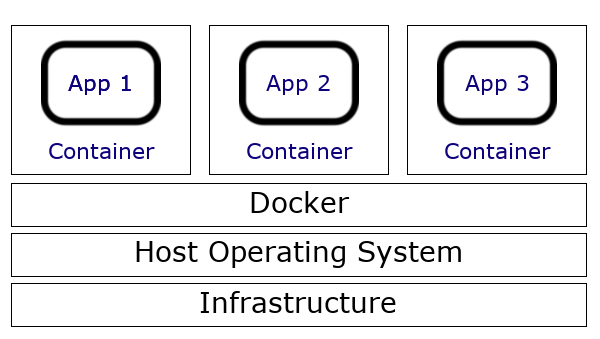
\includegraphics[width=1\textwidth]{containerization.png}
  \caption{Docker\index{Docker} application containers\index{Docker!container}.}
  \label{fig:containers}
\end{figure}\\
\newline
Such kind of solution is the reason why containerization\index{Containerization} is more performant and requires less resources than virtualization\index{Virtualization}. This concept is not new, containerization\index{Containerization} can be seen as a different type of managing virtualization\index{Virtualization}. From one side they provide an isolated\index{Isolation} and secure environment. From the other side, they are lighter than virtual machines. Other advantages of using application containers\index{Docker!container} are immutability\index{Immutability}, portability\index{Portability} and scalability\index{Scalability} \cite{bib:containers_features}.\\
\newline
Containers\index{Docker!container} are also often used in the CI pipelines\index{GitLab!pipeline}, where each stage has different container\index{Docker!container}. They also simplify working with legacy projects. This is because developers can do everything in a container\index{Docker!container}, i.e. they do not need to install dependencies\index{Dependencies} on their local machines. Often the versions between the time a legacy code has been written and ran again are significantly different. Hence, keeping such project in a container\index{Docker!container} solves the problem of incompatibility\index{Incompatibility} in dependencies\index{Dependencies} versioning when working with legacy projects.
\subsubsection{Compilers Rules}
There are two types of compilers used in this project, one for compiling TypeScript\index{TypeScript} and another one for Angular\index{Angular}. Nx\index{Nx} provides support for created components to have different settings on each single scope with a global compilers configuration file in an application root. The project of this application has one file for its global configuration \textit{.tsconfig.json}. In this file Angular\index{Angular} and TypeScript\index{TypeScript} compiler settings are defined.\\
\newline
Each of these separately defined modules (under \textit{libs} and \textit{src} contain actually three different compiler setting files as shown on Figure \ref{fig:simplified_architecture}). Considering an example one of \textit{libs} modules (e.g. \textit{home}), the structure is as follows:
\begin{itemize}
    \item \textbf{tsconfig.json} --- general specification of compilers settings for particular local scope.
    \item \textbf{tsconfig.lib.json} --- settings of compilers which apply only to the development environment. 
    \item \textbf{tsconfig.spec.json} --- settings of compilers which apply only to the testing environment, i.e. unit testing\index{Software!testing!unit} using Jest\index{Jest}.
\end{itemize}
For \textit{apps/ditectrev} the only difference is name of a file for the second settings, i.e. it is \textit{tsconfig.app.json}. This is a place for development settings of application's root components where the page is actually rendered. E2E\index{Software!testing!End-to-End (E2E)} tests (\textit{ditectrev-e2e}) have \textit{tsconfig.json} and \textit{tsconfig.e2e.json}. The second one works adequately to \textit{tsconfig.app.json}. The \textit{server} module has only \textit{tsconfig.json}. The \textit{functions} is without compiler settings, as it is used only for deployment and testing transpiled\index{Transpilation} project. Apart from that, TypeScript\index{TypeScript} compiler settings have been defined in global \textit{tsconfig.json}, from which all other files mentioned in this section inherits\index{Inheritance}. In case of a conflict for the same rule, the locally defined rules overwrites the global settings.\\
\newline
Default configuration for TypeScript\index{TypeScript} compiler is not that strict in terms of security. For that, several options in TypeScript\index{TypeScript} compiler in a JSON\index{JavaScript Object Notation (JSON)} format has to be enabled. These are specified in Listing \ref{lis:typescript_compiler}.\\
\newline
\begin{lstlisting}[language=json,firstnumber=1,label={lis:typescript_compiler},caption={TypeScript's compiler custom stricter rules.}][ht]
{
    "compilerOptions": {
        "alwaysStrict": true,
        "extendedDiagnostics": true,
        "noFallthroughCasesInSwitch": true,
        "noImplicitAny", true,
        "noImplicitThis", true,
        "noImplicitReturns": true,
        "noUnusedLocals": true,
        "noUnusedParameters": true,
        "strict": true,
        "strictBindCallApply": true,
        "strictFunctionTypes": true,
        "strictNullChecks": true,
        "strictPropertyInitialization": true
    }
}
\end{lstlisting}
All of them are disabled by default \cite{bib:typescript_compiler_settings} and might have positive impact on security of the application if turned on. Higher code quality is also achieved by following these rules. Explanation on the benefits to enable them for each option is given below:
\begin{itemize}
    \item \textbf{alwaysStrict} --- enable parsing strict mode with emitting \textit{"use strict"} for each file.
    \item \textbf{extendedDiagnostics} --- show more in-depth diagnostic information.
    \item \textbf{noFallthroughCasesInSwitch} --- report error when a \textit{switch/case} would fail.
    \item \textbf{noImplicitAny} --- disallow declarations and expressions with implied \textit{any} type.
    \item \textbf{noImplicitThis} --- raise an error when \textit{this} has implied \textit{any} type.
    \item \textbf{noImplicitReturns} --- throw an error when not all code paths in method returns a value.
    \item \textbf{noUnusedLocals} --- enable reporting an error when local variable would not be used.
    \item \textbf{noUnusedParameters} --- enable reporting an error if parameter of a method would not be used.
    \item \textbf{strict} --- all strict type checking options will be enabled.
    \item \textbf{strictBindCallApply} --- stricter checking for \textit{apply\footnote{Built-in JavaScript\index{JavaScript} method for calling a function.}}, \textit{bind\footnote{Built-in JavaScript\index{JavaScript} method for creating a function.}} and \textit{call\footnote{Built-in JavaScript\index{JavaScript} method for calling a function. The difference to \textit{apply} is only about taking arguments in a different way.}} methods.
    \item \textbf{strictFunctionTypes} --- disable bivariant parameter\index{Bivariant parameter} checking for function types. 
    \item \textbf{strictNullChecks} --- allow \textit{null} and \textit{undefined} types to be used only with themselves and \textit{any} type.
    \item \textbf{strictPropertyInitialization} --- ensure \textit{non-undefined} class properties are initialized in the constructor.
\end{itemize}
The option \textit{strict} in terms of security is crucial. By settings this to \textit{true} the application will enable seven strict type-checkings, i.e. \textit{alwaysStrict}, \textit{noImplicitAny}, \textit{noImplicitThis}, \textit{strictBindCallApply}, \textit{strictFunctionTypes}, \textit{strictNullChecks} and \textit{strictPropertyInitialization}. That way, most of these from Listing \ref{lis:typescript_compiler} will be enabled by this single line. \\
\newline
Angular's\index{Angular} compiler rules are defined in a different file, i.e. global \textit{tsconfig.lib.json}. The others \textit{tsconfig.lib.json} files inherits\index{Inheritance} from it. Listing \ref{lis:angular_compiler} presents a code snippet for Angular\index{Angular} compiler rules.
\begin{lstlisting}[language=json,firstnumber=1,label={lis:angular_compiler},caption={Important rules for Angular's\index{Angular} compiler.}][ht]
{
    "angularCompilerOptions": {
        "annotationsAs": "static fields",
        "annotateForClosureCompiler": true,
        "disableTypeScriptVersionCheck": false,
        "enableLegacyTemplate": false,
        "strictInjectionParameters": true,
        "strictMetadataEmit": true,
        "trace": true
    }
}
\end{lstlisting}
These following Angular\index{Angular} compiler options gives the following benefits:
\begin{itemize}
    \item \textbf{annotationsAs} --- enable more sophisticated tree shaking, e.g. Closure Compiler\footnote{Google's compiler for JavaScript\index{JavaScript} which outputs high quality and well-optimized JavaScript\index{JavaScript}.}\index{Closure Compiler} techniques.
    \item \textbf{annotateForClosureCompiler} --- this flag is required by the Closure Compiler\index{Closure Compiler}.
    \item \textbf{disableTypeScriptVersionCheck} --- TypeScript\index{TypeScript} version must be checked if set to \textit{false}. Setting this to \textit{true} would ignore errors about unsupported TypeScript\index{TypeScript} versions.
    \item \textbf{enableLegacyTemplate} --- make impossible to use deprecated \textit{<template>} tag to avoid collisions with element which has the same name in the DOM.
    \item \textbf{strictInjectionParameters} --- throw an error for parameters without possible to determine injection types.
    \item \textbf{strictMetadataEmit} --- emit errors for metadata, that otherwise would be ignored.
    \item \textbf{trace} --- show more information during compiling templates.
\end{itemize}
\subsubsection{Secure Development}
There are many factors developers should think about during the development phase in order to deliver secure software. Angular\index{Angular} offers protectsion from some of the attacks by default. However, there are also attacks which developers have to take care of such as broken access control, cryptographical\index{Cryptography} protocols weaknesses, Denial of Service (DoS)\index{Denial of Service (DoS)}/Distributed Denial of Service (DDoS)\index{Distributed Denial of Service (DDoS)}, known vulnerabilities\index{Vulnerabilities!Known Vulnerabilities}, security misconfiguration\index{Security!misconfiguration}, server malware\index{Malware} and many others. These attacks are not primarily related to the front-end\index{Front-end} layer. The background of these weaknesses could be hacking\index{Hacking}, human-prone mistakes, open source vulnerabilities\index{Vulnerabilities}, server-related issues and many others. Therefore, Angular\index{Angular} applications developed following the SSDLC\index{Secure Software Development Life Cycle (SSDLC)} should result to be more resistant on typical attacks.\\
\newline
An integral part of secure development is automation of security checks. This not only includes security testing\index{Security!testing}, but code quality checks too. Code smells\footnote{Set of common characteristics which specifies that the source code is not good enough and should be improved.} in the application can affect the security itself. A CI pipeline\index{GitLab!pipeline} with different type of tests challenges this problem and is presented on Figure \ref{fig:pipeline}. The pipeline\index{GitLab!pipeline}
 should has several stages with deployment only if tests are passed. Every change or more precisely every new \textit{git push} to the repository would indicate to run the whole pipeline\index{GitLab!pipeline} from start to end. In such a way that with every deployment the likelihood of delivering more secure application is higher.
\begin{figure}[ht]
  \centering
      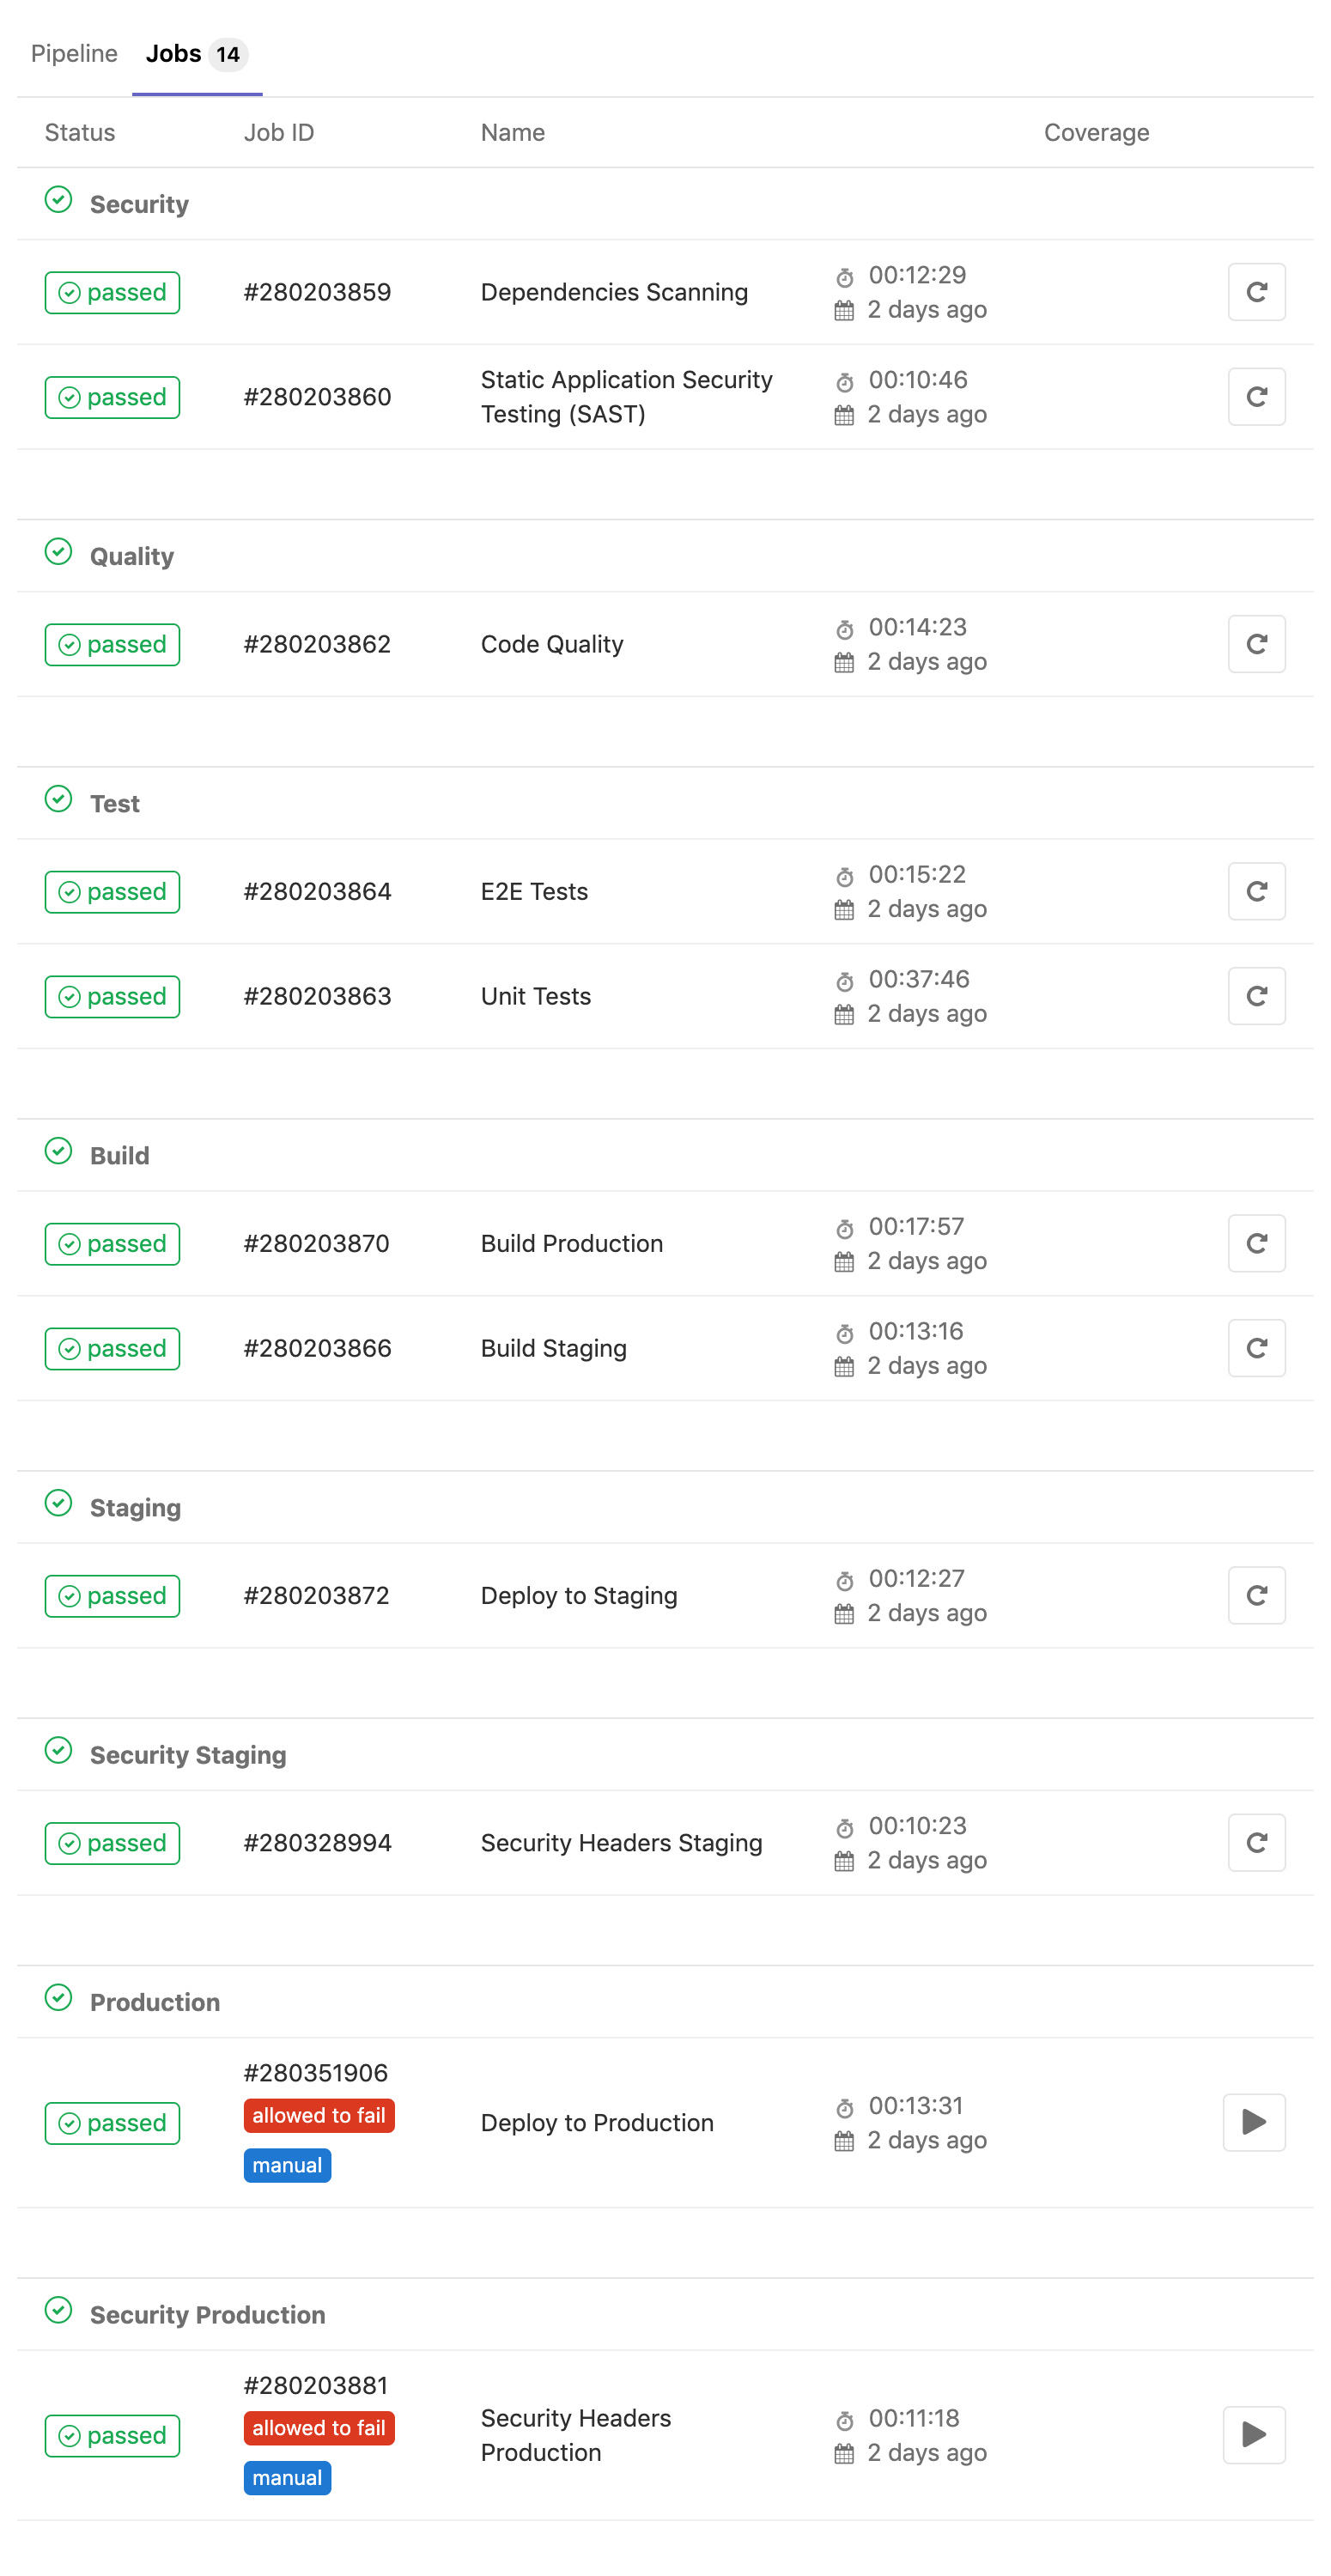
\includegraphics[width=.55\textwidth]{pipeline.png}
  \caption{Multistage GitLab CI\index{Continuous Integration (CI)} pipeline\index{GitLab!pipeline} of developed application.}
  \label{fig:pipeline}
\end{figure}\\
\newline
A crucial part of web application\index{Web Application} security is input validation\index{Validation}. For input validation\index{Validation!input} Angular\index{Angular} provides security in terms of input patterns for different types of inputs. However, it does not for file uploads --- this requires custom implementation by the developer. There are two main strategies to handle this problem:
\begin{enumerate}
    \item \textbf{Whitelisting} --- accept only specific types of files.
    \item \textbf{Blacklisting} --- reject listed files, accept all others.
\end{enumerate}
First of all, in both strategies executable files as well as too large files definitely should not be accepted. List of unsecure file patterns is long, especially including unordinary types of files. For this reason, whitelisting is a better strategy, because the system will accept only these kind of files which are supposed to be accepted. Moreover, the error handling\index{Error Handling} message should be rather general than detailed. By providing a detailed response the attacker might guess what kind of strategy is used.\\
\newline
It is worth noting that even icons might be a potential source of vulnerabilities\index{Vulnerabilities}. The modern standard for icons Scalable Vector Graphics (SVG)\index{Scalable Vector Graphics (SVG)} relies on a vector graphics rendering. This uses JavaScript\index{JavaScript} for scripting, which means it can be executed by a potential attacker. Data injections and XSS\index{Cross-Site Scripting (XSS)} attacks can be mitigated by implementing CSP\index{Content Security Policy (CSP)} in combination with Angular's built-in protection.
\subsubsection{Security Testing}\index{Security!testing}
\label{sec:security_testing}
Protection of software from hypothetical attacks is a primary goal for security testing\index{Security!testing}. Security is becoming an integral part of the SDLC\index{Software Development Life Cycle (SDLC)} since few years back, but it has been a topic of research for more than 15 years \cite{bib:software_security_testing}. Seven basic security concepts are authentication, authorization, availability, confidentiality, identification, integrity and non-repudiation. These are evaluated by different types of security tests \cite{bib:dast_vs_sast}. The most general approach is to divide them on two categories:
\begin{enumerate}
    \item \textbf{Dynamic Application Security Testing (DAST)\index{Software!testing!Dynamic Application Security Testing (DAST)}} --- also known as \textit{black box testing\index{Software!testing!black box}}, is executed in running application where the ethical hacker intentionally introduces fault injections to find weaknesses. In this scenario there is no access to the source code.
    \item \textbf{Static Application Security Testing (SAST)\index{Software!testing!Static Application Security Testing (SAST)}} --- also known as \textit{white box testing\index{Software!testing!white box}}, is performed during development to find security vulnerabilities\index{Vulnerabilities} in the source code without executing it.
\end{enumerate}
These two types of techniques can be done both automatically and manually. It depends on what is supposed to be tested, thus different tools are used for those. The core difference between them are presented in Table \ref{tab:sec_testing}. A hybrid approach, called \textit{grey box testing} is also sometimes distinguished between these two in which the security is tested by given partial information about the system.
\begin{table}[ht]
\hspace*{-2cm}
\centering
    \begin{tabular}{ | c | c |}
    \hline\multicolumn{1}{|c|}{\textbf{DAST}\index{Software!testing!Dynamic Application Security Testing (DAST)}} & \multicolumn{1}{c|}{\textbf{SAST}\index{Software!testing!Static Application Security Testing (SAST)}} \\ \hline
    Hacker approach & Developer approach \\ \hline
    Lack of knowledge about used technologies & Access to the source code \\ \hline
    Finds runtime and environment-related issues  & Does not find runtime and environment-related issues \\ \hline
    Typically used only in web \& mobile applications & Supported by almost all kinds of programming languages \\ \hline
    More expensive to fix & Cheaper to fix \\ \hline
    \end{tabular}
\caption{Difference between DAST\index{Software!testing!Dynamic Application Security Testing (DAST)} and SAST\index{Software!testing!Static Application Security Testing (SAST)} \cite{bib:dast_vs_sast}.}
\label{tab:sec_testing}
\hspace*{-2cm}
\end{table}\\
More recent approaches are Interactive Application Security Testing (IAST)\index{Interactive Application Security Testing (IAST)} and Runtime Application Self-Protection (RASP)\index{Runtime Application Self-Protection (RASP)}. The first one is a combination of DAST\index{Software!testing!Dynamic Application Security Testing (DAST)} and SAST\index{Software!testing!Static Application Security Testing (SAST)} which works inside the application. Vulnerabilities\index{Vulnerabilities} can be continuously monitored and identified, because these tests are performed right after the functional tests are done. Due to this fact it can be easily integrated into the CI/CD\index{Continuous Integration (CI)}\index{Continuous Delivery (CD)} pipelines\index{GitLab!pipeline}. That is why vulnerabilities\index{Vulnerabilities} are detected earlier than using the traditional SAST\index{Software!testing!Static Application Security Testing (SAST)} approach and the unsecure bundle can be automatically dropped from a potential deployment. Another advantage is the code coverage\index{Code Coverage} which includes also frameworks\index{Framework} and libraries.
RASP\index{Runtime Application Self-Protection (RASP)} also works inside the application, but it differs from the IAST\index{Interactive Application Security Testing (IAST)}. RASP\index{Runtime Application Self-Protection (RASP)} is more like a security tool per se, whilst IAST\index{Interactive Application Security Testing (IAST)} has more focus on the security testing itself. RASP\index{Runtime Application Self-Protection (RASP)} is included in the application, analyse it and in case of anomalies sends an issue alert or even blocks an application execution. In such a way it can thwart attacks automatically, especially important for these based on the recently discovered vulnerabilities\index{Vulnerabilities}.\\
\newline
Security testing\index{Security!testing} is an essential part of the SSDLC\index{Secure Software Development Life Cycle (SSDLC)}. Recent research shows that it is easier to implement it in an agile\index{Agile} project management frameworks\index{Framework} such as Scrum\index{Scrum} \cite{bib:framework_for_scrum, bib:pentesting_in_agile}. These findings provide an interesting conclusion. The authors suggests that even the chosen project management framework\index{Framework} might influence achieving different security levels during software development\index{Software!development}. This should be preceded by defining security risks\index{Security!risks} which influence on the decision what should be tested using what kind of techniques and tools.
\subsubsection{Continuous Security\index{Continuous Security}}
Nonstop monitoring of application in terms of security might be a challenging task. The CI/CD\index{Continuous Integration (CI)}\index{Continuous Delivery (CD)} apart improving productivity \cite{bib:cde_challenges, bib:cd_facebook, bib:ci_cd_all} can be helpful in automatic security tests. However, there might be a confusion between CI/CD acronyms. In order to understand the difference between them, it is important to define its meaning \cite{bib:ci_cd_all} and distinguish between these:
\begin{itemize}
    \item \textbf{Continuous Integration (CI)} --- integrating code in a shared repository. It builds and tests each commit change automatically\footnote{In some scenarios such as editing technical documentation in the source code repository it is not a desired behaviour. Automatic pipeline\index{GitLab!pipeline} build can be omitted. An example includes setting up a GitLab\index{GitLab} CI\index{Continuous Integration (CI)} command which would read Git\index{Git} commits containing information about skipping the build.}. It is part of continuous delivery as well as continuous deployment.
    \item \textbf{Continuous Delivery (CD)}\index{Continuous Delivery (CD)} --- releasing changes to production as quickly as possible by automatically pushing changes to a staging environment. From a staging based on certain conditions the application can be manually pushed to the production environment.
    \item \textbf{Continuous Deployment (CD or CDE)}\index{Continuous Deployment (CD or CDE)} --- goes one step further than continuous delivery. Deployment to production is fully automated.
\end{itemize}
Continuous security\index{Continuous Security}, similarly to continuous integration, should be an integral part of continuous delivery and continuous deployment. The security checks to achieve decent security level should be strict. Steps to achieve it are usually: container\index{Docker!container} and dependency\index{Dependencies} scanning, DAST\index{Software!testing!Dynamic Application Security Testing (DAST)} and SAST\index{Software!testing!Static Application Security Testing (SAST)}. More sophisticated methods could include: fuzzing\index{Fuzzing}, IAST\index{Interactive Application Security Testing (IAST)}, mutation testing\index{Software!testing!mutation} or RASP\index{Runtime Application Self-Protection (RASP)}.\\
\newline
From these three the most secure seems to be continuous delivery, where deployment from staging to production is done manually. The reason for that is even though pipelines\index{GitLab!pipeline} would pass all tests, then the application might be still not working correctly. Continuous deployment definitely speeds up time-to-production, but also contains some risks \cite{bib:security_cde}. The scenario for this could be for example when providing a wrong API key\index{Application Programming Interface (API)!key} in the environmental variables\index{Environmental Variable} of a CI\index{Continuous Integration (CI)} system. Even though locally everything worked correctly, it is always better deploy to staging. The environment is usually almost the same as the production one. Thus, it can be manually tested there and manually deployed to the production once the results of these tests will be positive. That is the reason why continuous delivery seems to be more safe and secure.
\subsection{Behavior-Driven Development}
Integration of unit tests\index{Software!testing!unit} into Angular\index{Angular} development environment is relatively easy due to its component-based architecture\index{Software!architecture!component-based}. Apart from that, Angular CLI\index{Angular!Command Line Interface (CLI)} generates the test files automatically when creating a new component. Together with a testing framework\index{Framework} it creates a nicely isolated\index{Isolation} structure of the application literally created for unit testing\index{Software!testing!unit}. Similarly to TDD\index{Test-Driven Development (TDD)} three main phases are defined: red\footnote{First phase of BDD\index{Behavior-Driven Development (BDD)}/TDD\index{Test-Driven Development (TDD)} when a test is failing.}, green\footnote{Improving unit test\index{Software!testing!unit} to pass the test case.} and refactor\footnote{Possible improvements of a unit test\index{Software!testing!unit}.}. In contrast to the TDD\index{Test-Driven Development (TDD)}, BDD\index{Behavior-Driven Development (BDD)} focuses more on how the application should behave for the end user. TDD\index{Test-Driven Development (TDD)} is more strictly about implementation of the functionality. The BDD\index{Behavior-Driven Development (BDD)} comes from the TDD\index{Test-Driven Development (TDD)}, but takes more flexible approach in the SDLC\index{Software Development Life Cycle (SDLC)}: test cases are not that strictly defined and are in a more human-readable format.\\
\newline
Fundamental part of the BDD\index{Behavior-Driven Development (BDD)} is Given-When-Then (GWT) approach \cite{bib:gwt_approach}, where
\begin{itemize}
    \item Given --- responsible for setting up a context.
    \item When --- describe an event.
    \item Then --- provide outcomes for the event.
\end{itemize}
The goal is to provide easy to understand and readable unit tests\index{Software!testing!unit}. By implementing BDD\index{Behavior-Driven Development (BDD)} it is easier to have more isolated\index{Isolation} structure of an application which gives enhancements in terms of security. The code maintenance becomes simpler. Clean separation of application's components is easier for debugging. It improves the chance to detect mistakes during development and to eliminate them before deployment. It can results in higher source code quality and less security flaws in it. The BDD\index{Behavior-Driven Development (BDD)} process also helps to focus on user expectations, thus by applying it developers are able to achieve better UX\index{User Experience (UX)}. Developers benefit from the fact that part of the application can be tested without completely compiling and deploying the whole application. Since a small piece of code (unit) is the target it checks if particular part of the application behaves as it is expected.
\newpage
\huge Chapter 5
\section {Implementation}
\normalsize Awareness of recent cybercrime\index{Cybercrime} activities is already a good first step to develop secure application. Identifying security risks\index{Security!risks} and implementing security measures for developed scenario is the next one. Architecture designed from a security point of view is an important factor of the application \cite{bib:secure_architecture}. Implementation of architecture, clean code\index{Clean code}, the DRY\index{Don't Repeat Yourself (DRY)} principle, programming best practices\index{Programming Best Practices}, SecDevOps\index{SecDevOps} and overall SSDLC\index{Secure Software Development Life Cycle (SSDLC)} process is challenging and yet another step. Carefully selected technologies with appropriate tools may be helpful in that stage. With security in mind, developers have to find trade-offs between modern techniques and mature solutions. Modern techniques have a newer point of view to resolve some kind of problems. However, mature solutions have been used for already some time and are considered to be more stable.
\subsection{Functionalities}
The application build as part of this research contains some functionalities typical for a modern web application\index{Web Application}. It has several views which contain content with associated logic behind. These are typical web application\index{Web Application} features such as input field complete with input validation\index{Validation!input}, interactive elements, small back-end\index{Back-end} and routing\index{Routing} functionality. Other notable functionalities are:
\begin{itemize}
    \item \textbf{Accessibility} --- the application supports assistive technology for users with disabilities. It has been achieved using Agastya\footnote{Software for improving websites' accessibility.}\index{Agastya}, semantic HTML\index{HyperText Markup Language (HTML)} and Web Accessibility Initiative's Accessible Rich Internet Applications specification (WAI-ARIA)\footnote{Technology which solves problem of reading web content for people with disabilities by adding special directives to the source code.}\index{Web Accessibility Initiative's Accessible Rich Internet Applications specification (WAI-ARIA)} \cite{bib:wai_aria}.
    \item \textbf{Analytics} --- every modern application tracks the user behaviour, the application also contains it. Google Analytics\index{Google!Analytics} and Hotjar\index{Hotjar} have been used as a technologies for this task by using Google Tag Manager\index{Google!Tag Manager}.
    \item \textbf{Internationalization} --- Google Translate\index{Google!Translate} with Oswald Labs Platform APIs\index{Application Programming Interface (API)} provides a way to smoothly integrate into an application automatic translation in more than 100 languages. It has been achieved implementing the Agastya\index{Agastya} software into the application.
    \item \textbf{Offline} --- a service worker\footnote{Script that runs in a background without interacting with a user.}\index{Service Worker} is part of the application to include PWA\index{Progressive Web Application (PWA)} characteristics.
    \item \textbf{Responsiveness} --- Responsive Web Design (RWD)\index{Responsive Web Design (RWD)} has been implemented using modern techniques of CSS\index{Cascading Style Sheets (CSS)} such as Flexbox Layout\index{Cascading Style Sheets (CSS)!Flexbox Layout} and Grid Layout\index{Cascading Style Sheets (CSS)!Grid Layout}. More precisely, its implementation in forms of directives called \textit{Angular-Flex Layout}\index{Angular!Flex Layout} has been used.
    \item \textbf{Rich front-end\index{Front-end}} --- significant number of integrations has been performed in order to provide appropriate UX\index{User Experience (UX)}. Many libraries and plugins in a form of external dependencies\index{Dependencies} have been used to achieve this effect.
\end{itemize}
Visualization of the application is attached to the thesis in the appendix \fullref{sec:appendices}. Some of these functionalities can be noticed from these screenshots. seen from the attached screenshots can be found in UI design elements.
\subsection{Technology Stack}
The application has been build using wide spectrum of technologies. They have been used from the development stage, through testing, ending up on production. These are the following:
\begin{itemize}
    \item \textbf{Core Framework}\index{Framework} --- fundamental part of this project is Angular\index{Angular} with its dedicated CLI\index{Angular!Command Line Interface (CLI)}. It consists of its own API\index{Application Programming Interface (API)} with number of useful methods for animations, compiling process, dependency injection\index{Dependency injection}, forms, handling HTTP\index{Hypertext Transfer Protocol (HTTP)}, routing\index{Routing}, service workers\index{Service Worker}, testing, validators\index{Validation} and more. This framework\index{Framework} supports most recent major browsers as of the time of writing this thesis \cite{bib:angular_browser_support}.
    \item \textbf{Cypress\index{Cypress} } --- efficient test runner for automated E2E\index{Software!testing!End-to-End (E2E)} tests, which can be used as all-in-one platform instead of few E2E\index{Software!testing!End-to-End (E2E)} tools.
    \item \textbf{Dependencies}\index{Dependencies} ---  external dependencies\index{Dependencies} installed during development in order to enrich the application functionalities or development experience. These can be code quality checks, external libraries, security testing\index{Security!testing} tools or UI\index{User Interface (UI)} improvements.
    \item \textbf{Docker\index{Docker}} --- software for running applications in an isolated\index{Isolation} environment (container\index{Docker!container}).
    \item \textbf{Firebase} --- development platform for mobile and web projects. The developed application has been deployed to Firebase Hosting\index{Firebase!hosting} which is supported by Google Cloud Platform (GCP)\footnote{Cloud computing services offered by Google.}\index{Google Cloud Platform (GCP)}. Other Firebase\index{Firebase} features which has been used includes: Cloud Firestore\footnote{Non relational (NoSQL)\index{Structured Query Language (SQL)!non SQL (NoSQL)} database for Firebase.}\index{Firebase!Cloud Firestore}, Cloud Functions for Firebase\index{Firebase!Cloud Functions for Firebase} and Cloud Storage for Firebase\footnote{Storage service offered by Google within Firebase.}\index{Firebase!Cloud Storage for Firebase}. These helped to create the application in a serverless\index{Serverless} technology, Firebase Security Rules\footnote{Set of security rules for Firebase databases.} was responsible for improving security\index{Security!improving}.
    \item \textbf{Git} --- distributed VCS\index{Version Control System (VCS)} widely used for source code versioning and tracking changes of code repository. Changes are send through HTTPS\index{Hypertext Transfer Protocol Secure (HTTPS)} or Secure Shell (SSH)\index{Secure Shell (SSH)} to source code repository where the project is stored.
    \item \textbf{GitLab} --- source code repository which embeds Git\index{Git} and provides an ecosystem for DevOps\index{DevOps} lifecycle. Contains features such CI\index{Continuous Integration (CI)}/CD\index{Continuous Delivery (CD)} integrations, code analysis, container registry, planning tool, project management, security, Source Code Management (SCM) and more. It also provides a secure way to store application secrets, such as passwords, secret API keys\index{Application Programming Interface (API)!key} and other sensitive properties in a form of environmental variables\index{Environmental Variable}.
    \item \textbf{Jest\index{Jest}} --- efficient platform used for unit testing\index{Software!testing!unit}. At this point of time this is currently one of the TDD\index{Test-Driven Development (TDD)}/BDD\index{Behavior-Driven Development (BDD)} frameworks\index{Framework} which integrates with Angular\index{Angular} seamlessly. The reason to choose Jest\index{Jest} is its perfectly matching construction to monolithic repositories.
    \item \textbf{NestJS}\index{NestJS} --- a Node.js\index{Node.js} framework\index{Framework} for building back-end\index{Back-end} web applications\index{Web Application}. It has been used to set up a minimalistic back-end\index{Back-end} with security configuration.
    \item \textbf{Nx\index{Nx}} --- extension for the Angular CLI\index{Angular!Command Line Interface (CLI)} for better management of Angular\index{Angular}-based large projects. It comes with specific architecture which promotes clean code\index{Clean code}, consistency, productivity and safety. This is equipped with code formatter, easier state management, simplified data persistence, static code analysis\index{Static Code Analysis}, visualization of dependencies\index{Dependencies} in a form of a graph and more useful features helpful during development.
    \item \textbf{RxJS\index{RxJS}} --- library for reactive programming which simplifies asynchronous programming. Functionalities such as filtering through glossary results and subscription for a newsletter were the use cases in this project.
    \item \textbf{Webpack}\index{webpack} --- module bundler for JavaScript\index{JavaScript}. Transcompiles\index{Transpilation} Angular\index{Angular} and TypeScript\index{TypeScript} code into JavaScript\index{JavaScript}. Webpack\index{webpack} also enables to work with yet unsupported natively new standards of ECMAScript\index{ECMAScript} and translate it into executable by the browsers JavaScript\index{JavaScript}. Other customizations are also possible, mainly based on self-written scripts with corresponding plugins.
\end{itemize}
\subsection{Improving Security\index{Security!improving}}
There are several well known techniques to increase security in web environments. The first one is to enable HTTPS\index{Hypertext Transfer Protocol Secure (HTTPS)} on the domain of the web application\index{Web Application}. This common practice protects against Man-In-The-Middle (MITM) attacks\footnote{Type of attack in which an attacker is between two communication parties, reads and possible alter the communication between them.}\index{Man-In-The-Middle (MITM)!attack}. In that case only breaking encryption or gathering cryptographical\index{Cryptography} secrets seems to be the only way for an attacker to break the system.\\
\newline
However, there are still more techniques to perform a MITM attack\index{Man-In-The-Middle (MITM)!attack}. It applies even to websites served over HTTPS\index{Hypertext Transfer Protocol Secure (HTTPS)} unless user does not has installed plugins like HTTPS Everywhere\footnote{Extensions for major browsers which serves websites over HTTPS\index{Hypertext Transfer Protocol Secure (HTTPS)} only.}\index{Hypertext Transfer Protocol Secure (HTTPS)!Everywhere}. In one of the possible scenarios an attacker could make a request to a real website over HTTPS\index{Hypertext Transfer Protocol Secure (HTTPS)} and forward it to the victim over unencrypted HTTP\index{Hypertext Transfer Protocol (HTTP)}. To mitigate this issue HTTP Strict Transport Security (HSTS) policy mechanism\index{HTTP Strict Transport Security (HSTS)!policy mechanism} is used. The HSTS header\index{HTTP Strict Transport Security (HSTS)!header} forbids the browser to make calls to a known website without Secure Socket Layer (SSL)\index{Secure Socket Layer (SSL)}/TLS\index{Transport Layer Security (TLS)}. It does works only for users who visited the website. In order to have HSTS policy mechanism\index{HTTP Strict Transport Security (HSTS)!policy mechanism} working for users visiting the website for the first time a \textit{preload} flag is required. By doing this a SSL\index{Secure Socket Layer (SSL)}/TLS\index{Transport Layer Security (TLS)} stripping\footnote{Type of MITM attack\index{Man-In-The-Middle (MITM)!attack} that forces a victim's browser to communicate over unencrypted HTTP.} is mitigated.\\
\newline
Nowadays, several countermeasures\index{Countermeasures} are provided by default from some cloud hosting companies. For example, Firebase\index{Firebase} which is being used in this research to host the application has some of them. The CDN\index{Content Delivery Network (CDN)} provided by a Firebase\index{Firebase} partner includes basic (D)DoS\index{Denial of Service (DoS)}\index{Distributed Denial of Service (DDoS)} server protections. A reverse proxy\index{Reverse Proxy} with a 10 MB payload size is also in place for the serverless\index{Serverless} back-end\index{Back-end}. Cloud Functions for Firebase\index{Firebase!Cloud Functions for Firebase} also have rate, resource and time limits by default. Logging and monitoring is also provided in the administrator dashboard. On the other side, Angular\index{Angular} provides data sanitization for injection attacks as well as CSRF\index{Cross-Site Request Forgery (CSRF)} and XSS\index{Cross-Site Scripting (XSS)} protection on the client-side. However, there are still defense mechanisms that developers have to take into account in the development stage.
\subsubsection{Input Validation\index{Validation!input}}
Input fields from HTML\index{HyperText Markup Language (HTML)} need to be validated\index{Validation}. Angular\index{Angular} has built-in support for input validation\index{Validation!input}. It can be easily achieved what kind of input it is required from the user as Listing \ref{lis:input_validators} shows.
\begin{lstlisting}[language=JavaScript,firstnumber=1,label={lis:input_validators},caption={Input validators\index{Validation!input} in Angular\index{Angular}.}][ht]
Validators.email; // Accept only e-mail pattern.
FileValidator.maxContentSize(20971520); // Limit size of files to 20 MB.
Validators.maxLength(512); // Allow maximum 512 characters.
Validators.minLength(2); // Require at least 2 characters.
Validators.pattern('^[0-9]*$'); // Accept only numbers.
Validators.required; // Mark this field as required
\end{lstlisting}
These rules are quite straightforward. The developer only has to decide which validator\index{Validation} will be applied to a particular input field. This decreases the risk compared to a manual implementation. Custom input validation\index{Validation!input} implementations in a form of regular expressions are considered to be complicated. Wrongly implemented regular expressions could compromise the server.
\subsubsection{File Upload Attack Prevention\index{File Upload Attack!prevention}}
Unfortunately, Angular\index{Angular} does not provide validators\index{Validation} for file upload\index{Validation!file upload} type. The HTML\index{HyperText Markup Language (HTML)} side should whitelist accepted formats like on Listing \ref{lis:html_input_types}. This in combination to Angular's\index{Angular} file upload size validators\index{Validation!file upload} is a current solution for defining types of accepted files for upload.
\begin{lstlisting}[language=HTML,firstnumber=1,label={lis:html_input_types},caption={Cloud Storage for Firebase\index{Firebase!Cloud Storage for Firebase} security rules for file upload.}][ht]
<ngx-mat-file-input [accept]="['.doc', '.docx', '.jpg', '.jpeg', '.pdf', '.png', '.xls', '.xlsx']" (change)="uploadFile($event)" formControlName="fileUploader" multiple type="file">
\end{lstlisting}
Such validation\index{Validation} is easy to bypass. The file after all is uploaded to a cloud storage and this is where a proper validation\index{Validation} is required. Listing \ref{lis:cloud_storage_rules} shows the back-end validation\index{Validation!back-end}. The back-end validation cannot be omitted. Accepted files are limited to accepted formats using Multipurpose Internet Mail Extensions (MIME)\footnote{Standard for Internet formats.}\index{Multipurpose Internet Mail Extensions (MIME)} content types and a designated amount of files size. In such a way unrestricted file upload is handled on front-end\index{Front-end} and back-end\index{Back-end} side with limiting the size. Limiting file types decreases the risk of executing dangerous types of files which might led to execution of malicious scripts on the server. Setting boundaries of file size protects from DoS\index{Denial of Service (DoS)} due to large file upload.
\begin{lstlisting}[language=JavaScript,firstnumber=1,label={lis:cloud_storage_rules},caption={Cloud Storage for Firebase file upload security rules.}][ht]
// Allow write files Firebase Storage, only if:
// 1) File is no more than 20 MB
// 2) Content type is in one of the following formats: .doc, .docx, .jpg, .jpeg, .pdf, .png, .xls, .xlsx.
allow write: if request.resource.size <= 20 * 1024 * 1024
        && (request.resource.contentType.matches('application/msword')
        || request.resource.contentType.matches('application/vnd.openxmlformats-officedocument.wordprocessingml.document')
        || request.resource.contentType.matches('image/jpg')
        || request.resource.contentType.matches('image/jpeg')
        || request.resource.contentType.matches('application/pdf')
		    || request.resource.contentType.matches('image/png')
        || request.resource.contentType.matches('application/vnd.ms-excel')
        || request.resource.contentType.matches('application/vnd.openxmlformats-officedocument.spreadsheetml.sheet'))
\end{lstlisting}
\subsubsection{Security Headers}\index{Security!header}
An effective way to handle various of security weaknesses within JavaScript-related back-ends\index{Back-end} is by using a dependency\index{Dependencies} called \textit{Helmet}\index{Helmet}. Helmet helps in a relatively easy way to modify many HTTP headers\index{Hypertext Transfer Protocol (HTTP)!header} related with security and privacy. Its initialization implies adding protection into seven different attacks. The remaining ones have to be set up manually. Listing \ref{lis:security_headers} clearly presents the logic behind it written in NestJS\index{NestJS}.
\begin{lstlisting}[language=JavaScript,firstnumber=1,label={lis:security_headers},caption={Declaration of security headers in NestJS.}][ht]
import * as express from 'express';
import { Express } from 'express';
const helmet = require('helmet');

const expressApp: Express = express(); // Create Express instance.

expressApp.use(helmet()); // Enable Helmet's 7 default middleware protections, i.e. dnsPrefetchControl, frameguard, hidePoweredBy, hsts, ieNoOpen, noSniff and xssFilter.

// Preload HTTP Strict Transport Security (HSTS).
expressApp.use(
  helmet.hsts({
    includeSubDomains: true, // Must be enabled, so "preload" will work.
    maxAge: 31536000, // In seconds, one year.
    preload: true
  })
);

expressApp.use(helmet.permittedCrossDomainPolicies()); // Prevent Adobe Flash and Adobe Acrobat from loading content.

// Enforce to expect Certificate Transparency (CT) for 24 hours.
expressApp.use(
  helmet.expectCt({
    enforce: true,
    maxAge: 24 * 60 * 60 // In seconds, regard it for max 24 hours.
  })
);

// Limit website features by implementing Feature Policy.
expressApp.use(
  helmet.featurePolicy({
    features: {
      fullscreen: ["'self'"],
      payment: ["'none'"],
      syncXhr: ["'none'"]
    }
  })
);

server.use(helmet.noCache()); // Disable client-side caching.
server.use(helmet.referrerPolicy({ policy: 'same-origin' })); // Send Referer header only for pages on the same origin.
\end{lstlisting}
Initialization of this \index{Cybercrime}\index{Dependencies} (line seven) implies that these following middleware\index{Middleware} will inform HTTP headers\footnote{However, if particular browser does not support certain header it will not be enforced.}\index{Hypertext Transfer Protocol (HTTP)!header} how the browser should behave. The following behaviour is expected from the browser:
\begin{itemize}
    \item \textbf{dnsPrefetchControl} --- disable DNS\index{Domain Name System (DNS)} prefetching in the browsers (sets \textit{X-DNS-Prefetch-Control} to \textit{off}).
    \item \textbf{frameguard} --- mitigate clickjacking\footnote{Tricking victim to click on certain element which attacker controls. This element might be invisible or masked.}\index{Clickjacking} attacks (sets \textit{X-Frame-Options} to \textit{SAMEORIGIN}).
    \item \textbf{hidePoweredBy} --- hide used on the website technological stack (removes \textit{X-Powered-By}).
    \item \textbf{hsts} --- enforce keeping users on HTTPS\index{Hypertext Transfer Protocol Secure (HTTPS)} (turns on \textit{Strict-Transport-Security}).
    \item \textbf{ieNoOpen} --- inform Internet Explorer\index{Internet Explorer} no to execute downloads in a client site's context (sets \textit{X-Download-Options} to \textit{noopen}).
    \item \textbf{noSniff} ---  prevent browsers from trying to guess (\textit{sniff}) a MIME\index{Multipurpose Internet Mail Extensions (MIME)} type (sets \textit{X-Content-Type-Options} to \textit{nosniff}).
    \item \textbf{xssFilter} --- prevent reflected XSS\index{Cross-Site Scripting (XSS)} attack by (sets \textit{X-XSS-Protection} to \textit{1; mode=block}).
\end{itemize}
However, there are still a number of headers left which can be set to increase the security:
\begin{itemize}
    \item \textbf{contentSecurityPolicy} --- whitelist scripts which can be loaded in an application (sets \textit{Content-Security-Policy}).
    \item \textbf{crossdomain} --- prevent handling data across domains (sets \textit{X-Permitted-Cross-Domain-Policies} to \textit{none}). Especially it focus on Adobe Flash and Adobe Acrobat which can load content from other sites.
    \item \textbf{expectCt} --- browser will expect Certificate Transparency (CT)\footnote{Technique for auditing and monitoring identity certificates (also known as public key certificate or digital certificate). It detects fake and malicious SSL\index{Secure Socket Layer (SSL)} certificates.}\index{Certificate Transparency (CT)} from the requested website (sets \textit{Expect-CT}).
    \item \textbf{featurePolicy} --- restrict which features the application can use (sets \textit{Feature-Policy}).
    \item \textbf{noCache} --- disable browser caching (modifies \textit{Cache-Control}, \textit{Expires}, \textit{Pragma} and \textit{Surrogate-Control}).
    \item \textbf{referrerPolicy} --- disable forwarding information about site origin when user moves from one site to another (modifies \textit{Referer} and \textit{Referrer-Policy}). This is a privacy enhancement rather than a security issue.
\end{itemize}
One option has not been used at all, i.e. \textit{hpkp} (HTTP Public Key Pinning (HPKP)\index{Hypertext Transfer Protocol (HTTP)!Public Key Pinning (HPKP)}). The new \textit{Expect-CT} header is considered to be more flexible and safer \cite{bib:expect-ct}. Both of them mitigate the same attack.
\subsubsection{Content Security Policy}\index{Content Security Policy (CSP)}
Previous listings does not include implementation of CSP. This particular security header\index{Security!header} itself required more source code than all the others headers. Listing \ref{lis:csp} presents CSP\index{Content Security Policy (CSP)} which limits allowed external scripts which can be executed in the application. The short comments inform for which integrated technology it is required, whilst the others are self-explanatory.
\begin{lstlisting}[language=JavaScript,firstnumber=1,label={lis:csp},caption={CSP for developed application.}][ht]
import * as express from 'express';
import { Express } from 'express';
const helmet = require('helmet');

const expressApp: Express = express(); // Create Express instance.

expressApp.use(
  helmet.contentSecurityPolicy({
    browserSniff: false, // Disable browser sniffing.
    directives: {
      baseUri: ["'self'"], // Restricts use of the "<base>" tag to origin (without subdomains). This directive doesn't use "default-src" as fallback, thus by default it allows anything.
      blockAllMixedContent: true, // Prevent loading any assets using HTTP when the page is loaded using HTTPS.
      childSrc: [
        "'self'", // Default policy for valid sources for web workers and nested browsing contexts loaded using elements such as "<frame>" and "<iframe>": allow all content coming from origin (without subdomains).
        'https://vars.hotjar.com' // Hotjar.
      ],
      connectSrc: [
        "'self'", // Default policy for restricting the URLs which can be loaded using script interfaces: allow all content coming from origin (without subdomains).
        'https://agastya-version.oswaldlabs.com', // Agastya.
        'https://firebasestorage.googleapis.com', // Cloud Storage for Firebase.
        'https://firestore.googleapis.com', // Cloud Firestore.
        'https://platform-beta.oswaldlabs.com', // Agastya.
        'https://www.google-analytics.com', // Universal Analytics (Google Analytics).
        'https://*.hotjar.com:*', // Hotjar.
        'https://vc.hotjar.io:*', // Hotjar.
        'wss://*.hotjar.com' // Hotjar.
      ],
      defaultSrc: [
        "'none'" // Default policy for fallback for the other CSP fetch directives [Link of these: https://developer.mozilla.org/en-US/docs/Web/HTTP/Headers/Content-Security-Policy/default-src]: disallows everything.
      ],
      fontSrc: [
        "'self'", // Default policy for specifiying valid sources for fonts loaded using "@font-face": allow all content coming from origin (without subdomains).
        'https://fonts.gstatic.com', // Google Fonts.
        'https://script.hotjar.com' // Hotjar.
      ],
      formAction: ["'self'"], // Default policy for restricting the URLs which can be used as the target of a form submissions from a given context: allow all content coming from origin (without subdomains). This directive doesn't use "default-src" as fallback, thus by default it allows anything.
      frameAncestors: ["'self'"], // Default policy for specyfing valid parents that may embed a page using "<frame>", "<iframe>", "<object>", "<embed>", or "<applet>". This directive doesn't use "default-src" as fallback, thus by default it allows anything. This is basically clickjacking protection.
      frameSrc: [
        "'self'", // Default policy for specyfing valid sources for nested browsing contexts loading using elements such as "<frame>" and "<iframe>": allow all content coming from origin (without subdomains).
        'https://agastya-version.oswaldlabs.com', // Agastya.
        'https://vars.hotjar.com', // Hotjar.
        'https://www.google.com' // reCAPTCHA.
      ],
      imgSrc: [
        "'self'", // Default policy for specyfing valid sources of images and favicons: allow all content coming from origin (without subdomains).
        'https://www.google-analytics.com', // Universal Analytics (Google Analytics).
        'https://www.googletagmanager.com', // Google Tag Manager.
        'https://www.google.com', // reCAPTCHA.
        'https://script.hotjar.com' // Hotjar.
      ],
      manifestSrc: ["'self'"], // Default policy for specyfing which manifest can be applied to the resource: allow all content coming from origin (without subdomains).
      objectSrc: ["'none'"], // Default policy for specyfing valid sources for the "<object>", "<embed>", and "<applet>" elements. It also influences "pluginType" by disallowing all of them. The "pluginType" directive doesn't use "default-src" as fallback, thus by default it allows anything.
      scriptSrc: [
        "'self'", // Default policy for valid sources for JavaScript: allow all content coming from origin (without subdomains).
        "'unsafe-eval'", // Unsecure, but required due to Angular's SSR.
        'https://agastya-version.oswaldlabs.com', // Agastya.
        'https://ditectrev.us15.list-manage.com', // MailChimp.
        'https://platform.oswaldlabs.com', // Agastya.
        'https://platform-beta.oswaldlabs.com', // Agastya.
        'https://script.hotjar.com', // Hotjar.
        'https://static.hotjar.com', // Hotjar.
        'https://ssl.google-analytics.com', // Universal Analytics (Google Analytics).
        'https://www.google-analytics.com', // Universal Analytics (Google Analytics).
        'https://www.googletagmanager.com', // Google Tag Manager.
        'https://www.google.com', // reCAPTCHA.
        'https://www.gstatic.com' // reCAPTCHA.
      ],
      styleSrc: [
        "'self'", // Default policy for valid sources for stylesheets: allow all content coming from origin (without subdomains).
        "'unsafe-inline'", // Unsecure, but required in order to render styles generated by Angular compiler, which on SSR are generated as inline styles.
        'https://fonts.googleapis.com' // Google Fonts.
      ],
      upgradeInsecureRequests: true // Block loading of active/passive content over insecure FTP/HTTP by "upgrading" the connection to secure SFTP/HTTPS.
    }
  })
);
\end{lstlisting}
\subsubsection{Others}
\label{sec:security_others}
The application has number of other preventions for explicit security improvements. Some of them has been included in a GitLab pipeline\index{GitLab!pipeline} before it is deployed. These include:
\begin{itemize}
    \item Error handling\index{Error Handling} without revealing error details to the client.
    \item Importing application modules from a path, thus avoiding loading using variables. It could have originated from user input which might be harmful.
    \item Limit concurrent requests using Express middleware\index{Express!middleware}. It can slow down brute-force attacks\index{Brute-force} significantly, in practice making them useless.
    \item Logging behaviour of different errors and events which helps in proper monitoring.
    \item Principle of least privilege for database access.
    \item Requesting manual interaction (also known as automation prevention, i.e. reCAPTCHA\footnote{System to validate\index{Validation} humans and robots.}\index{reCAPTCHA}) for expected paths of bot attacks.
    \item Running Node.js\index{Node.js} inside a Docker\index{Docker} container\index{Docker!container} as a non-root user which by default runs as \textit{root}.
    \item Prevention of CSRF\index{Cross-Site Request Forgery (CSRF)} attacks by adding \textit{X-XSRF-TOKEN} header only if the \textit{XSRF-TOKEN} cookie\index{Cookies} was generated on the back-end\index{Back-end}.
    \item Static code analysis\index{Static Code Analysis} to catch code security bugs and programming mistakes in an early stage. Embedded in a pipeline\index{GitLab!pipeline}, helped to detect and eliminate over a dozen issues. There were two exceptions from the default rules: \textit{no-non-null-assertion}\footnote{Non-null assertions are required within passing data for some scenarios in a compilers strict mode.} and \textit{no-shadowed-variable}\footnote{Unit test\index{Software!testing!unit} case specific for mocking one of external dependencies\index{Dependencies}.}. A single mistake in the source code will cause the GitLab pipeline\index{GitLab!pipeline} to fail.
    \item Scanning for known vulnerabilities\index{Vulnerabilities!Known Vulnerabilities} and eliminating them as fast as possible. During the project development about 1,500 known vulnerabilities\index{Vulnerabilities!Known Vulnerabilities} have been detected and eliminated. This is an integral part of a CI pipeline\index{GitLab!pipeline}. The configuration has been set up strictly, i.e. even one low vulnerability\index{Vulnerabilities} causes a failing deployment.
    \item Secure cookies\index{Cookies} and sessions management. This prevents cookies\index{Cookies} from being transferred through HTTP\footnote{Even if the application is served via HTTPS\index{Hypertext Transfer Protocol Secure (HTTPS)} it is possible.}\index{Hypertext Transfer Protocol (HTTP)}, it disables cookie forgery\footnote{Forging an authentication without actually doing it.}\index{Cookies!forgery} and hides revealed by default in sessions application technology.
    \item Storing sensitive data such as application secrets in environmental variables\index{Environmental Variable}.
    \item Whitelist API keys\index{Application Programming Interface (API)!key} for external services and from which domains they are allowed to be called.
\end{itemize}
There are also different elements which implicitly improves security. These are code formatting, E2E\index{Software!testing!End-to-End (E2E)} tests, unit tests\index{Software!testing!unit} and following all types of programming best practices\index{Programming Best Practices}.
\subsection{Clean Code\index{Clean code}}
An important part of programming best practices\index{Programming Best Practices} is clean code\index{Clean code}. Good documentation, high readability, naming conventions and proper objects grouping are examples of the core ideas. Developers arguably spend more time on reading the code than writing code. That is why providing a clean working environment is important. It reduces onboarding time for new members, decreases maintenance time and simplifies debugging \cite{bib:cleancode}. Strongly typed languages like TypeScript\index{TypeScript} should take advantage of its nature and use types. Examples of bad and clean code\index{Clean code} shows Listings \ref{lis:bad_code} and \ref{lis:clean_code}.
\begin{lstlisting}[language=JavaScript,firstnumber=1,label={lis:bad_code},caption={Bad code in TypeScript\index{TypeScript}.}][ht]
// Case 1.
var x;
x = 5;

// Case 2.
currentDate = new Date();

// Case 3.
private crscn(renderer) {
  ico = new Mesh(new IcosahedronGeometry(40, 4), new MeshStandardMaterial({
    color: new Color('#061371'),
    emissive: new Color('#3f51b5'),
    transparent: true,
    wireframe: true
  }));
  this.scene.add(ico);
  return ico;
}
\end{lstlisting}
\begin{lstlisting}[language=JavaScript,firstnumber=1,label={lis:clean_code},caption={Clean code\index{Clean code} in TypeScript\index{TypeScript}.}][ht]
// Case 1.
const usersNumber: number = 5;

// Case 2.
public currentDate: Date = new Date();

// Case 3.
public scene: Scene = new Scene(); // Create the scene.

/**
  * @description Create scene of this animation.
  * @param {renderer} - the renderer object to display scenes using WebGL.
  * @returns {Mesh}
  */
public createScene(renderer): Mesh {
  const radius: number = 40;
  const detail: number = 4;
  
  // Create material object with properties for surfaces with highlights.
  const material: MeshStandardMaterial = new MeshStandardMaterial({
    color: new Color('#061371'), // Color of the material.
    emissive: new Color('#3f51b5'), // Color of emissive light of the material.
    transparent: true, // Make transparent bacground.
    wireframe: true // Render geometry as wireframe.
  });

  const icosphere: Mesh = new Mesh(new IcosahedronGeometry(radius, detail), material); // Create the icosahedron geometry.
  this.scene.add(icosphere); // Add  icosahedron geometry to the scene.
  return icosphere;
}
\end{lstlisting}
These two listings represents part of the source code used in the application. Even though the code will be working for all of these examples, there are several programming flaws. Analysis of the source code quality is based on three cases:
\begin{itemize}
    \item \textbf{Case 1} --- uninitialized variable \textit{x} with the \textit{var} keyword. Lack of initialization of variables for some languages causes that it contains a certain value, but it is unpredictable. It is known to be one of the most frequent programming mistakes resulting with security flaws. Especially, it is present in programming languages for which stack variables are not initialized by default, such as C/C++\index{C}\index{C++} \cite{bib:cwe_variables}. A good practice is to avoid it and declare it explicitly. Another mistake which is strongly related with JavaScript\index{JavaScript} is to use a problematic keyword \textit{var}. It has several problems like scoping, possibility of re-declarations and updating as well as hoisting\footnote{JavaScript's\index{JavaScript} default behavior of moving declarations to the top.}. Instead, \textit{let} should be considered as a preferred way to declare variables since the time of introducing ES2015\index{ES2015}. The new syntax later is transpiled\index{Transpilation} to the executable by browsers JavaScript\index{JavaScript}. Variables with constant values should use \textit{const} keyword.
    \item \textbf{Case 2} --- implicit modifiers which in TypeScript\index{TypeScript} can be: \textit{private}, \textit{protected} and \textit{public}. They help to limit exposure of classes, functions and variables. It is crucial especially if working with two different languages in the same project. In some languages the default modifiers policy is different. An example could be C\#, where every property has the \textit{private} modifier, whilst in TypeScript\index{TypeScript} it is \textit{public}. A real world scenario includes front-end\index{Front-end} on Angular\index{Angular}, React\index{React} or Vue.js\index{Vue.js}. These can use TypeScript\index{TypeScript}, in Angular\index{Angular} it is de facto a standard, with back-end\index{Back-end} in ASP.NET Core\index{ASP.NET Core} which is using C\#\index{C\#}. Being explicit about the modifiers solves the problem of remembering what kind of policy is in which language. These can be avoid confusing when working with cross-technological projects.
    \item \textbf{Case 3} --- function definition without a stated return type, poorly documented and containing unintuitive names without proper convention. An explicit declaration with correctly defined type which this method has to return is cleaner to understand what to expect from this function. Secondly, in the first example it is not correctly documented, it is especially important whilst working with third party libraries. It helps to understand what kind of behaviour it causes, good documentation can be achieved using JSDoc\index{JSDoc} markup language. Thirdly, the good code listing outsources object properties, which helps to understand the technical context. Lastly, correct names with convention is much better than shortcuts or combined words without uppercase first letters. Conventions like \textit{lowerCamelCase} are a good approach for variables which supposed to contain more complex objects.
\end{itemize}
One of the advantages of TypeScript\index{TypeScript} is having the ability to use a better code intelligence tool due to the static type-checking. In the two listings above in the explicit source code it can be noticed what kind of advantage it gives. Even though the code executed by the browsers is JavaScript\index{JavaScript}, TypeScript\index{TypeScript} helps improving security\index{Security!improving} in the development stage. Potentially made mistakes leading to bugs due to the nature of JavaScript\index{JavaScript} can be largely eliminated using TypeScript\index{TypeScript}. Positive effect of using types have been recently researched with the conclusion that it decreases number of bugs by 15\% \cite{bib:type_study}. Apart from bug-catching abilities, strongly typed languages also simplifies maintenance of an application once the project grows and reduces the risk of overwriting properties.
\newline
Writing clear source code also minimizes the risk of code smells which at the end affects security of the application. Some general basic principles \cite{bib:cleancode} are:
\begin{itemize}
    \item Avoid code smells like dead code, framework\index{Framework} core modifications, hard-coding, large classes, long conditional statements etc.
    \item Classes and methods should be not too large, follow the DRY\index{Don't Repeat Yourself (DRY)} and SRP\index{Single Responsibility Principle (SRP)} rules.
    \item Use easy to follow logic within application.
    \item Adhere to naming convention recommended by the framework\index{Framework} or language, follow it consistently and uniformly.
    \item Grouping variables by importance, name and prefixes.
    \item Use meaningful, i.e. intention-revealing, pronounceable names with picking up one word per concept.
    \item Use proper source code comments in order to understand what each class or method is responsible for.
    \item Unit tests\index{Software!testing!unit} are written and are an integral part of the codebase.
    \item Use verbs for function names and nouns for classes and attributes.
\end{itemize}
\subsection{Unit Testing\index{Software!testing!unit}}
A fundamental part of BDD\index{Behavior-Driven Development (BDD)} is unit testing\index{Software!testing!unit}. Tests should be simple and easy to read for non-technical people. Unit tests\index{Software!testing!unit} also have best practices to follow, one of them is the RITEway\cite{bib:riteway}. The first four letters are abbreviations of \textbf{R}eadable, \textbf{I}solated/\textbf{I}ntegrated, \textbf{T}horough, \textbf{E}xplicit. These names clearly indicate in what kind of manner unit tests\index{Software!testing!unit} should be written. An application with correctly written unit tests\index{Software!testing!unit} should follow the RITEway and BDD\index{Behavior-Driven Development (BDD)}. High level of test coverage might improve overall security of an application. Often it is considered to have at least 80\% in order to say it is a reasonable code coverage\index{Code Coverage} \cite{bib:efficient_code_coverage}. It reduces risk of possible software defects which could occur after deployment without unit tests\index{Software!testing!unit} embedded in the SDLC\index{Software Development Life Cycle (SDLC)}.
\newline
Besides if this is TDD\index{Test-Driven Development (TDD)} or BDD\index{Behavior-Driven Development (BDD)} every unit test\index{Software!testing!unit} should answer five questions \cite{bib:unit_test_questions}, such as:
\begin{enumerate}
    \item What has been tested?
    \item What should it do?
    \item What was the actual output?
    \item What was the expected output?
    \item How can the test be reproduced?
\end{enumerate}
Following the RITEway and having answers for these questions helps to write tests with keeping the code to absolute minimum. Isolation\index{Isolation} and minimization is a sign of a good unit test\index{Software!testing!unit}. The only extension to isolated\index{Isolation} unit tests\index{Software!testing!unit} are when components are based on external dependencies\index{Dependencies}. Then to test it properly, mocking\footnote{Creating objects that simulates behaviour of real objects.} technique has to be involved in the process.\\
\newline
A core benefit of implementing unit testing\index{Software!testing!unit} is that the logic cannot be changed accidentally which may cause existing functionality to break. Doing unit tests\index{Software!testing!unit} also helps to improve the design of application's architecture. However, there are also less obvious implications of it. One of them is that tests themselves helps to structure how the application should behave. Moreover, by implementing TDD\index{Test-Driven Development (TDD)}/BDD\index{Behavior-Driven Development (BDD)} developers should be also be more confident about their work.
\subsection{Server-Side Rendering}
Usually Angular\index{Angular} executes source code in the browser, but it is also possible to run Angular\index{Angular} code on the server-side using Angular\index{Angular} Universal. This technique is called \textit{SSR}\index{Server-Side Rendering (SSR)}, its main benefit is to improve Search Engine Optimization (SEO)\index{Search Engine Optimization (SEO)} and enhance performance, especially on low-powered devices. This requires from developers custom modifications, because by default \textit{Client-Side Rendering} (CSR)\index{Client-Side Rendering (CSR)} is used, differences between SSR\index{Server-Side Rendering (SSR)} and CSR\index{Client-Side Rendering (CSR)} are multiple \cite{bib:ssr_vs_csr} and are represented by Table \ref{tab:ssr_vs_csr}.
\begin{table}[ht]
\hspace*{-2.8cm}
\begin{center}
    \begin{tabular}{ | c | l | l |}
    \hline
    \multicolumn{1}{|c|}{\textbf{Step}} & \multicolumn{1}{c|}{\textbf{Description for CSR}} & \multicolumn{1}{c|}{\textbf{Description for SSR}} \\ \hline
    0. & \multicolumn{2}{c|}{Requesting a page} \\ \hline
    \multicolumn{1}{|c|}{1.} & \multicolumn{1}{c|}{Server sends response to the browser} & \multicolumn{1}{c|}{Servers sends ready to be rendered HTML} & & & \multicolumn{1}{c|}{response to the browser} \\ \hline
    \multicolumn{1}{|c|}{2.} & \multicolumn{2}{c|}{Browser downloads the assets (content files, JavaScript\index{JavaScript})} \\ \hline
    3. & \multicolumn{2}{c|}{Application is executed in the browser} \\ \hline
    4. & \multicolumn{2}{c|}{Page is interactable and viewable} \\ \hline
    \end{tabular}
\caption{Steps to load page using CSR\index{Client-Side Rendering (CSR)} and SSR\index{Server-Side Rendering (SSR)} .}
\label{tab:ssr_vs_csr}
\end{center}
\hspace*{-2cm}
\end{table}\\
\newline
The main difference is in the process of rendering page contents. In the SSR\index{Server-Side Rendering (SSR)} approach the page is displayed even before it will be ready to interact. In the CSR\index{Client-Side Rendering (CSR)} Angular\index{Angular} makes the application ready, once it is clickable and interactable. This small difference makes different results in page speed tests in favor of SSR\index{Server-Side Rendering (SSR)} which might be important in enterprise applications. The SSR\index{Server-Side Rendering (SSR)} for SPA\index{Single-Page Application (SPA)} is currently becoming more popular and has been used.
\subsection{Version Control System}
Practical part of this research requires significant amount of source code to write. For this purpose Git\index{Git} has been used as a VCS\index{Version Control System (VCS)} and a Git\index{Git} repository managed by GitLab\index{GitLab}\footnote{Available to see at \url{https://gitlab.com/danieldanielecki/thesis_app} once permission will be received, last access: 26 August 2019.} has been set up to simplify development. Git\index{Git} is currently the most popular VCS\index{Version Control System (VCS)} of modern software development\index{Software!development}. Semantic commits help to review this repository on later stage. Therefore, convention of seven main behaviours has been kept for source code of the application:
\begin{itemize}
    \item \textbf{Add:} --- typical commit for adding new logic into the application.
    \item \textbf{Change:} --- something has been changed in the project.
    \item \textbf{Delete:} --- certain piece of code has been dropped. 
    \item \textbf{Fix:} --- some functionality has been repaired.
    \item \textbf{Improve:} --- code formatting, documentation, error handling\index{Error Handling}, security or any other improvement.
    \item \textbf{Refactor:} --- part of the source code is restructured. 
    \item \textbf{Update:} --- at least one of application's dependencies\index{Dependencies} has been updated.
\end{itemize}
As a good practice commits are done often with small changes which helps to standardize versioning. However, there is one more important factor of using repository hosted on GitLab. This is its good integration with GitLab\index{GitLab} CI\index{Continuous Integration (CI)}, a system for CI/CD\index{Continuous Integration (CI)}\index{Continuous Delivery (CD)} development practice with various of tools it provides.\\
\newline
Versioning of the application is achieved using so-called semantic versioning. The general idea behind it is to keep in Git\index{Git} tag numbering MAJOR.MINOR.PATCH \cite{bib:semver}, where:
\begin{itemize}
    \item \textbf{MAJOR} --- the most influential additions, e.g. 1.X.X implies first deployable version.
    \item \textbf{MINOR} --- this includes more general changes in the application.
    \item \textbf{PATCH} --- a small improvement has been added.
\end{itemize}
The repository should have been configured with permissions for certain collaborators. In such a way that users making changes will require to have the correct permissions. Making \textit{master} as a protected branch is also required and a good practice.
\subsection{Deployment}
The application is deployed on Firebase Hosting\index{Firebase!hosting} --- service for provided by Google for serving web content. Pipelines\index{GitLab!pipeline} have been set up and synchronized with Firebase\index{Firebase} to provide automatic deployment. There are two implemented types of hosting environments:
\begin{enumerate}
    \item \textbf{Staging}\footnote{\url{https://thesisapp-dev.firebaseapp.com/}, last access: 26 August 2019.} --- used for testing purposes before deployment to production.
    \item \textbf{Production}\footnote{\url{https://thesisapp-16048.firebaseapp.com/}, last access: 26 August 2019.} --- the final destination for deployment of the application.
\end{enumerate}
Applications hosted on Firebase\index{Firebase} by default are equipped with: built-in protection against (D)DoS\index{Denial of Service (DoS)}\index{Distributed Denial of Service (DDoS)} attacks, Content Delivery Network (CDN)\footnote{System of geographically distributed proxy servers working together in order to provide fast delivery of web content.}\index{Content Delivery Network (CDN)}, GZIP compression\footnote{Method to improve performance for serving web content faster.}\index{GZIP compression}, HTTP/2\index{Hypertext Transfer Protocol (HTTP)!HTTP/2} support\footnote{Fully multiplexed version of HTTP\index{Hypertext Transfer Protocol (HTTP)!header} network protocol.}, Nginx\index{Nginx} web server\index{Web Server}, reverse proxy\footnote{Type of proxy server with additional layer of abstraction which forwards clients requests to appropriate back-end\index{Back-end} server.}\index{Reverse Proxy} and SSL\index{Secure Socket Layer (SSL)} certificate\footnote{Data files which cryptographically\index{Cryptography} allow a secure connection between browser and web server\index{Web Server}.}.\\
\newline
Firebase\index{Firebase} provides its own CLI\index{Firebase!Command Line Interface (CLI)} to deploy an application using a terminal. It also smoothly integrates with a CI\index{Continuous Integration (CI)} system. The code is then transpiled\index{Transpilation} which is described in detail in the next section. Webpack\index{webpack} is responsible for minification\footnote{Remove unnecessary characters in order to minimize the codebase size.} and obfuscation\footnote{Making source code more difficult for humans to read and understand.}\index{Obfuscation} of the source code into a form of ready-to-deploy bundle. This bundle is wrapped in a GitLab container\index{GitLab!container} and shipped to the GitLab pipeline\index{GitLab!pipeline}. The CI system performs automatic tests and once these are passed sends the container\index{Docker!container} to a staging environment. The staging environment is for manual tests to check if the added logic works as expected in a real environment. It has to be tested by a developer or tester. If approved, then the application is shipped to production by manually informing the CI\index{Continuous Integration (CI)} system about it. The whole communication and server content is through secure connection served over HTTPS\index{Hypertext Transfer Protocol Secure (HTTPS)} or SSH\index{Secure Shell (SSH)}.
\subsection{Transpilation\index{Transpilation}}
\label{sec:transpilation}
Once the implementation part has been finished the last concept to clarify is how actually the source code is executed. A process called \textit{transpilation\index{Transpilation}} is performed, this is a different than traditional compilation. Compiler translates language from high level programming language to its lower representation, e.g. C\#\index{C\#} to Microsoft Intermediate Language (MSIL)\index{Microsoft Intermediate Language (MSIL)} or Java\index{Java} to Java bytecode\index{Java bytecode}. In the transpilation\index{Transpilation} process the written source code is compiled from one programming language into another, but with a similar level of abstraction, e.g. CoffeeScript\index{CoffeeScript} to JavaScript\index{JavaScript}.\\
\newline
There are different module systems as described in the \fullref{sec:module} section. Nevertheless which one would be specify to work with during development, ES5\index{ES5} must and has been specified as a target platform. Currently, that is the standard compatible with all major browsers \cite{bib:es5_browser_support}. Webpack\index{webpack} is the tool which in the following project has been used during this research to bundle this technological stack and perform the last step before deployment to have runnable SPA\index{Single-Page Application (SPA)}. More precisely, webpack\index{webpack} firstly calls the TypeScript\index{TypeScript} compiler, then the Angular\index{Angular} compiler and finally builds the bundle during the build time (using AOT\index{Ahead-of-Time (AoT)}). This is how TypeScript\index{TypeScript} using ES2015\index{ES2015} modern techniques are translated from the Angular\index{Angular} project into JavaScript\index{JavaScript} interpretable by the browser.
\newpage
\huge Chapter 6
\section{Security Analysis\index{Security!analysis}}
\normalsize The evaluation of security of an application is an integral part of SecDevOps\index{SecDevOps} and SSDLC\index{Secure Software Development Life Cycle (SSDLC)} methodologies. Security testing\index{Security!testing} of the application is performed in three different ways. With full access to the source code (SAST\index{Software!testing!Static Application Security Testing (SAST)}/white box testing\index{Software!testing!white box}), without any access to the source code (DAST\index{Software!testing!Dynamic Application Security Testing (DAST)}/black box testing\index{Software!testing!black box}) and with limited access to the source code (gray box testing\index{Software!testing!gray box}).
\subsection{Static Application Security Testing}\index{Software!testing!Static Application Security Testing (SAST)}
First of all the source code of the application developed as part of this research is investigated. Some of the techniques have been automated in a GitLab pipeline\index{GitLab!pipeline} presented by Figure \ref{fig:pipeline}. Thus, the summary concludes some part of the pipeline\index{GitLab!pipeline} as well as manual code review. The derived conclusions are:
\begin{itemize}
    \item E2E tests\index{Software!testing!End-to-End (E2E)} could cover more elements of the application. One test has been excluded from the GitLab pipeline\index{GitLab!pipeline} due to an unknown incompatibility in the GitLab\index{GitLab} environment. Locally the test passed.
    \item Files for webpack's\index{webpack} browser and server logic are separated. They could have been merged into one file, because webpack\index{webpack} enables to have separated logic for client-side and server-side from a single file.
    \item High result of coverage in unit tests\index{Software!testing!unit} does not covers all application's logic due to Angular's CLI\index{Angular!Command Line Interface (CLI)} bug \cite{bib:angular_coverage}. This bug causes that code coverage\index{Code Coverage} report generated by Angular's CLI\index{Angular!Command Line Interface (CLI)} shows executed code. Adding test cases for the logic which was not executed gives full code coverage\index{Code Coverage} of certain component. One test have been excluded, i.e. \textit{not found} component due to problematic testing a Three.js\index{Three.js}\footnote{JavaScript\index{JavaScript} library for 3D browser graphics.}. This graphics library interacts with DOM\index{Document Object Model (DOM)} intensively and causes problems with the testing platform Jest\index{Jest}. The reason for that is Jest is using specific type of DOM\index{Document Object Model (DOM)}, i.e. JSDOM\footnote{Vanilla JavaScript implementation of DOM\index{Document Object Model (DOM)}, which aims to speed up execution of logic placed inside it.}\index{JSDOM}.
    \item Imports for routing\index{Routing} have long relative paths which could have been improved by adding Nx\index{Nx} logic to handle this. The compiler showed this as an improvement in terms of a code quality.
    \item Most possible strict compiler rules have been applied.
    \item No known vulnerabilities\index{Vulnerabilities!Known Vulnerabilities} were found out of 918.296 dependencies\index{Dependencies} checked.
    \item Old secrets have been found in the GitLab repository. These have been submitted accidentally when changing hiding secrets strategy. However, the credentials has have changed immediately due to the reason that they will be in the repository forever.
    \item Static analysis of source code has been passed with two exceptions described in the \fullref{sec:security_others} section, i.e. \textit{no-non-null-assertion} and \textit{no-shadowed-variable}. Security rules for static analysis has been applied.
\end{itemize}
\subsection{Dynamic Application Security Testing\index{Software!testing!Dynamic Application Security Testing (DAST)}}
There are several methods to check the application's security from a hacker's point of view. These include amongst others information gathering, manual testing and scanning techniques. A comprehensive security analysis\index{Security!analysis} is presented in the following sections.
\subsubsection{Information Gathering}
When it comes to penetration testing\index{Software!testing!penetration} the first step is gathering information about the target system. Kali Linux\footnote{Distribution of Linux\index{Linux} designed for security testing\index{Security!testing}.}\index{Linux!Kali} with its penetration tools has been used for this. First of all, port scanning has been performed using nmap\footnote{Network scanner which sends packets and analyzes its responses.}\index{Nmap}. From 1.000 scanned ports, the 80 and 443 ports gave some information. Port 80 showed that allowed HTTP\index{Hypertext Transfer Protocol (HTTP)!header} methods are GET\index{Hypertext Transfer Protocol (HTTP)!GET request}, HEAD\index{Hypertext Transfer Protocol (HTTP)!HEAD request}, POST\index{Hypertext Transfer Protocol (HTTP)!POST request} and OPTIONS\index{Hypertext Transfer Protocol (HTTP)!OPTIONS request}. It was determined that the proxy might be redirecting requests. It also detected Varnish\index{Varnish} --- a caching tool. It was revealed that port 443 was served by Nginx\index{Nginx} as a web server\index{Web Server} and it was possible to retrieve several cryptographic\index{Cryptography} properties about the SSL\index{Secure Socket Layer (SSL)} certificate. The type of public key used was Rivest–Shamir–Adleman (RSA)\index{Rivest–Shamir–Adleman (RSA)} encryption with 2048 bits which holds a valid certificate for one year. The signature algorithm used was SHA256withRSAEncryption with HTTPS challenge\index{Hypertext Transfer Protocol Secure (HTTPS)!challenge} \textit{tls-alpn}. Most of the certificate information can be also found from a Mozilla Firefox\index{Mozilla!Firefox} browser. The configuration is the recommended compatibility as of the time of writing this thesis \cite{bib:ssl_compatibility}.  It did also find out that HTTP/2\index{Hypertext Transfer Protocol (HTTP)!HTTP/2} was used and a TCP\index{Transmission Control Protocol (TCP)} sequence prediction difficulty with a score of 17 was determined. According to nmap documentation \cite{bib:nmap_documentation, bib:nmap_source_code}, the result 17 is hard to break and thus considered to be secure.\\
\newline
The data mining tool Maltego\index{Maltego} found information about the actual network infrastructure. It showed that the CDN\index{Content Delivery Network (CDN)} was operated by Fastly Network Operations. It located \textit{ns-cloud-c1.googledomains.com} as the DNS\index{Domain Name System (DNS)} for the domain \textit{thesisapp-16048.firebaseapp.com}. Personal data was hidden and showed only business details of Google.\\
\newline
Wappalyzer\index{Wappalyzer} is a tool to discover technologies used on certain website. The front-end\index{Front-end} technologies were revealed, but not the back-end\index{Back-end} (for which Express\index{Express} and Node.js\index{Node.js} are used). It also did not show information about Nginx\index{Nginx} as a web server\index{Web Server}. However, this had been already discovered using nmap\index{Nmap}.\\
\newline
More investigation has been provided by Nikto\index{Nikto}. This is a scanner with in-depth analysis about web servers\index{Web Server}. The interesting logs are presented on Listing \ref{lis:nikto_logs} and shows some potential findings:
\begin{lstlisting}[language=json,firstnumber=1,label={lis:nikto_logs},caption={Nikto logs.}][ht]
+ The Content-Encoding header is set to "deflate" this may mean that the server is vulnerable to the BREACH attack.
+ /phpEventCalendar/file_upload.php: phpEventCalendar 1.1 and prior are vulnerable to file upload bug.
+ /contents/extensions/asp/1: The IIS system may be vulnerable to a DOS, see https://docs.microsoft.com/en-us/security-updates/securitybulletins/2002/MS02-018 for details.
+ OSVDB-4598: /members.asp?SF=%22;}alert(223344);function%20x(){v%20=%22: Web Wiz Forums ver. 7.01 and below is vulnerable to Cross Site Scripting (XSS)\index{Cross-Site Scripting (XSS)}. http://www.cert.org/advisories/CA-2000-02.html.
+ /servlet/com.unify.servletexec.UploadServlet: This servlet allows attackers to upload files to the server.
+ OSVDB-3233: /index.html.ee: Apache default foreign language file found. All default files should be removed from the web server\index{Web Server} as they may give an attacker additional system information.
+ OSVDB-3233: /index.html.it: Apache default foreign language file found. All default files should be removed from the web server\index{Web Server} as they may give an attacker additional system information.
+ /151.101.1.195.tar: Potentially interesting archive/cert file found.
+ /thesisapp-16048firebaseapp.jks: Potentially interesting archive/cert file found.
+ /thesisapp-16048firebaseapp.tgz: Potentially interesting archive/cert file found.
+ /backup.egg: Potentially interesting archive/cert file found.
+ /thesisapp-16048.firebaseapp.egg: Potentially interesting archive/cert file found.
+ OSVDB-3092: /trafficlog/: This might be interesting...
+ OSVDB-3092: /user/: This might be interesting...
+ OSVDB-3092: /users/: This might be interesting...
+ OSVDB-3092: /webaccess.htm: This might be interesting...
+ OSVDB-3092: /webaccess/access-options.txt: This might be interesting...
+ OSVDB-3093: /database/metacart.mdb+: This might be interesting... has been seen in web logs from an unknown scanner.
+ OSVDB-3093: /OA_JAVA/Oracle/: Oracle Applications portal pages found.
+ OSVDB-3093: /OA_JAVA/servlet.zip: Oracle Applications portal pages found.
+ OSVDB-3093: /OA_JAVA/oracle/forms/registry/Registry.dat: Oracle Applications portal pages found.
+ 7864 requests: 0 error(s) and 109 item(s) reported on remote host
+ End Time:           2019-08-17 23:02:55 (GMT0) (2676 seconds)
\end{lstlisting}
There are several potential interesting files and information about possible vulnerabilities\index{Vulnerabilities} on the server-side. Interesting are the findings about two different web servers\index{Web Server}, i.e. Apache\index{Apache} and Internet Information Services (IIS)\index{Internet Information Services (IIS)}. Even though the application is served by Nginx\index{Nginx}, it looks like the Firebase infrastructure\index{Firebase!infrastructure} uses mixed technologies. This includes also a Java\index{Java} and a PHP\index{PHP} stack.\\
\newline
Network security investigation revealed that neither DNSSEC\index{Domain Name System Security Extensions (DNSSEC)} nor firewall\index{Firewall} is enabled for the application.
\subsubsection{Web Scanners}
Another method for security scanning includes online web scanning for typical web vulnerabilities\index{Vulnerabilities}. The application has been tested by several of these, i.e. Checkbot: SEO, Web Speed \& Security Tester\footnote{\url{https://chrome.google.com/webstore/detail/checkbot-seo-web-speed-se/dagohlmlhagincbfilmkadjgmdnkjinl?hl=en}, last access: 27 August 2019.}\index{Checkbot: SEO, Web Speed \& Security Tester}, CryptCheck\footnote{\url{https://tls.imirhil.fr/https/thesisapp-16048.firebaseapp.com}, last access: 27 Augus 2019.}\index{CryptCheck}, ImmuniWeb\footnote{\url{https://www.immuniweb.com/websec/?id=Oy27vLRH}, last access: 26 August 2019.}\index{ImmuniWeb}, Mozilla Observatory\footnote{\url{https://observatory.mozilla.org/analyze/thesisapp-16048.firebaseapp.com}, last access: 29 August 2019.}\index{Mozilla!Observatory}, Pentest-Tools\footnote{\url{https://pentest-tools.com/home}, last access: 26 August 2019.}\index{Pentest-Tools}, Security Headers\footnote{\url{https://securityheaders.com/?q=https://thesisapp-16048.firebaseapp.com}, last access: 26 August 2019.}\index{Security!Headers}, SiteCheck\footnote{\url{https://sitecheck.sucuri.net/results/https/thesisapp-16048.firebaseapp.com}, last access: 26 August 2019.}\index{SiteCheck}, Qualys SSL Labs\footnote{\url{https://www.ssllabs.com/ssltest/analyze.html?d=thesisapp-16048.firebaseapp.com&s=151.101.1.195}, last access: 26 August 2019.}\index{Qualys SSL Labs}. All of the scans provided excellent results for the developed application. Table \ref{tab:web_scanners} presents grading score for all these web scanners.
\begin{table}[ht]
\centering
    \begin{tabular}{ | c | c |}
    \hline
    \multicolumn{1}{|c|}{\textbf{Name of a web scanner}} & \multicolumn{1}{c|}{\textbf{Score}} \\ \hline
    Checkbot: SEO, Web Speed\index{Checkbot: SEO, Web Speed \& Security Tester} \& Security Tester & 92\% \\ \hline
    CryptCheck\index{CryptCheck} & A \\ \hline
    ImmuniWeb\index{ImmuniWeb} & A \\ \hline
    Mozilla Observatory\index{Mozilla!Observatory} & A+ \\ \hline
    Pentest-Tools\index{Pentest-Tools} & Low security risk \\ \hline
    Security Headers\index{Security!Headers} & A \\ \hline
    SiteCheck\index{SiteCheck} & Low security risk \\ \hline
    Qualys SSL Labs\index{Qualys SSL Labs} & A+ \\ \hline
    \end{tabular}
\caption{Web scanners results for developed application.}
\label{tab:web_scanners}
\end{table}\\
One of them --- Mozilla Observatory\index{Mozilla!Observatory} has been integrated in GitLab pipeline\index{GitLab!pipeline} with a minimum result to pass 100 out of 100. Due to some additional security configuration the score actually was above the result of 100. The general score shows Figure \ref{fig:observatory1}, whilst more in-depth analysis Figure \ref{fig:observatory2}.
\begin{figure}[ht]
  \centering
      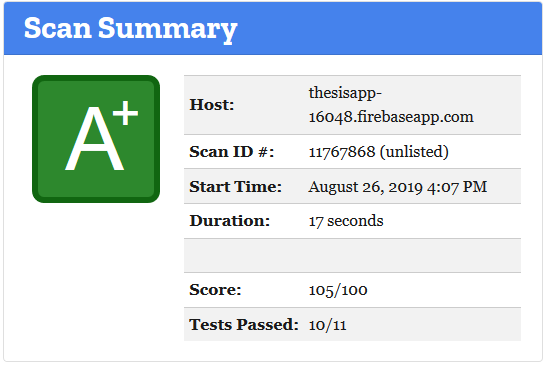
\includegraphics[width=0.45\textwidth]{observatory1.png}
  \caption{General security analysis\index{Security!analysis} score by Mozilla Observatory\index{Mozilla!Observatory}.}
  \label{fig:observatory1}
\end{figure}
\begin{figure}[ht]
  \centering
      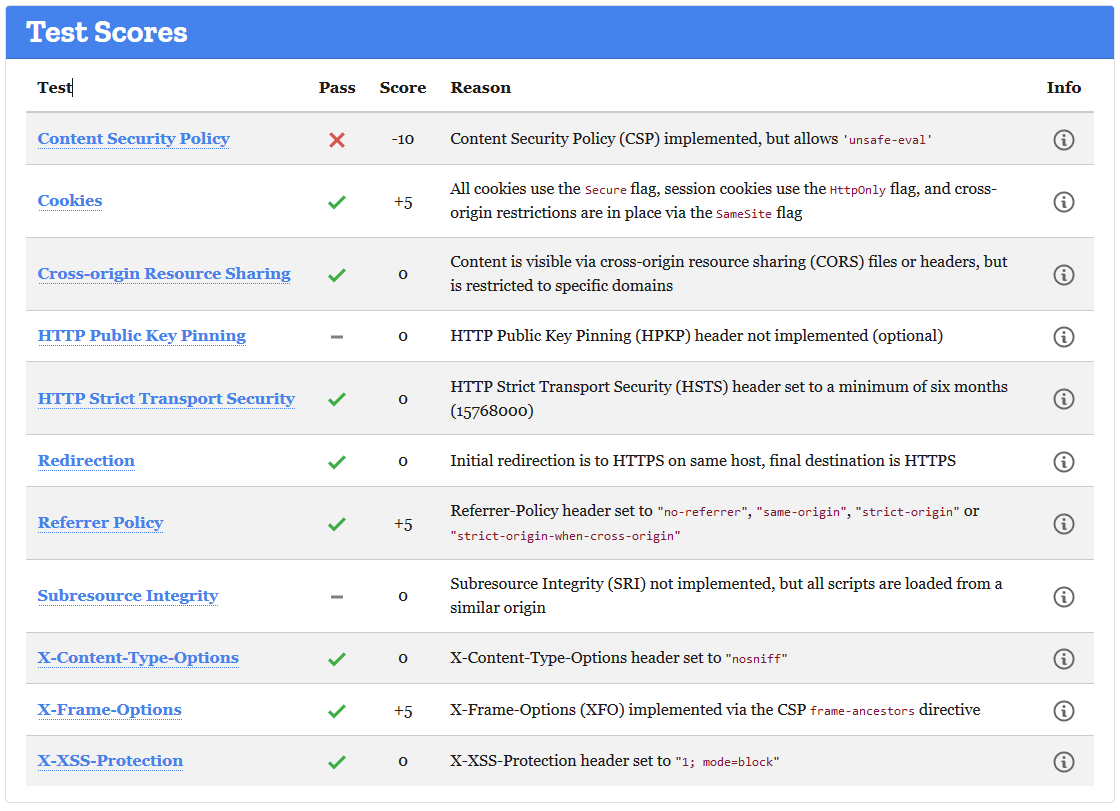
\includegraphics[width=0.75\textwidth]{observatory2.png}
  \caption{In-depth security analysis\index{Security!analysis} by Mozilla Observatory\index{Mozilla!Observatory}.}
  \label{fig:observatory2}
\end{figure}
\newpage
The CSP shows \textit{unsafe-eval} and \textit{unsafe-inline} which is caused by Angular's\index{Angular} SSR\index{Server-Side Rendering (SSR)}. The first finding can be denoted from the Figure \ref{fig:observatory2}, whilst the second in details of the scan by following the link \url{https://observatory.mozilla.org/analyze/thesisapp-16048.firebaseapp.com} (last access: 29 August 2019). When Angular\index{Angular} renders page on the server it performs inline styling. Disabling \textit{unsafe-eval} in CSP\index{Content Security Policy (CSP)} caused the application did not work properly. Thus, for SSR\index{Server-Side Rendering (SSR)} these two are required to render the application correctly. It clearly shows that for security weakness when using Angular\index{Angular} with SSR\index{Server-Side Rendering (SSR)}.
\newpage
\subsubsection{Skipfish\index{Skipfish}}
Out of many penetration testing\index{Software!testing!penetration} one of them provided unique insights. The reconnaissance tool Skipfish\index{Skipfish} was able to detect many things, which most of the other tools even did not note. Findings presents Figure \ref{fig:skipfish} presents.
\begin{figure}[ht]
  \centering
      \includegraphics[width=0.6\textwidth]{skipfish.png}
  \caption{Skipfish results.}
  \label{fig:skipfish}
\end{figure}\\
The first three which all are related with vector injection are considered to have a high risk.  Investigation of these issues revealed niche attack vectors known from fuzzing\index{Fuzzing}. This technique provides invalid, random and unexpected inputs. The possible attack vectors had different characters to some paths of the application, often images. These were for example paths to images with additional endings such as \textit{/""}, \textit{`true`} or \textit{/sfish>'>"<sfish><\%2Fsish>}. Unknown paths were also part of the result, i.e. \url{https://thesisapp-16048.firebaseapp.com/F.c/"`true`"}. This is interesting and niche finding. It clearly shows that there will be always certain attacks which are difficult to find and mitigate. Skipfish\index{Skipfish} was also able to detect several others as seen on the Figure \ref{fig:skipfish}. The next serious result is about external content, but this is not surprising since several APIs\index{Application Programming Interface (API)} are used. This is controlled by CSP\index{Content Security Policy (CSP)} and should be not harmful. Medium risk contains bypassing directory listing restrictions, whilst all others checks are positive with one exception. This is about failing when fetching a resource, it might be an error in application or in network during the test. It could be because sometimes this attack was stopped due to exceeding rate limit (100 connections per 15 minutes).
\subsubsection{Stress Testing\index{Software!testing!stress}}
Robustness of software beyond usual limits can determine DoS\index{Denial of Service (DoS)}. SlowHTTPTest\footnote{Tool for simulation of DoS\index{Denial of Service (DoS)} attacks on an application layer.}\index{SlowHTTPTest} showed good results for all four types of attacks simulation. Each of the simulation have taken different amount of time with 2.000 connections for each of them. During the tests the target server was available for around 98\% of the time of test. The attacks simulations were: Apache Killer\footnote{Sending many HTTP GET requests\index{Hypertext Transfer Protocol (HTTP)!GET request}\index{Apache!Killer} with enormous number of \textit{Byte Ranges} eventually causing running out of memory of  the server. This attack is also known as RANGE.}, Slowloris\footnote{Overwhelming a victim's server by opening and keeping many simultaneous HTTP\index{Hypertext Transfer Protocol (HTTP)} connections. This attack is also known as SLOW HEADERS\index{SLOW HEADERS}}\index{Slowloris}, R-U-Dead-Yet\footnote{Scanning a website for an embedded web forms. This attack also known as SLOW BODY\index{SLOW BODY}}\index{R-U-Dead-Yet} and SLOW READ\footnote{Sending many HTTP\index{Hypertext Transfer Protocol (HTTP)}\index{SLOW READ} requests and reading it very slowly or even not at all.}. Apache Killer\index{Apache!Killer} took the shortest amount of time, i.e. 49 seconds. After that time all connections were closed and server was available for 100\% duration of the test. Slowloris\index{Slowloris} took 648 seconds to close all connections. During that test between 279 and 293 seconds the server was not available. SLOW READ\index{SLOW READ} took 4683 seconds and no anomalies have been reported. The R-U-Dead-Yet\index{R-U-Dead-Yet} was that one which caused web server\index{Web Server} unavailable for the longest time. The server was not available for around 26-28 seconds out of 277 seconds of the test. The R-U-Dead-Yet\index{R-U-Dead-Yet} attack simulation is shown in Figure \ref{fig:ru_dead_yet}.
\begin{figure}[ht]
  \centering
      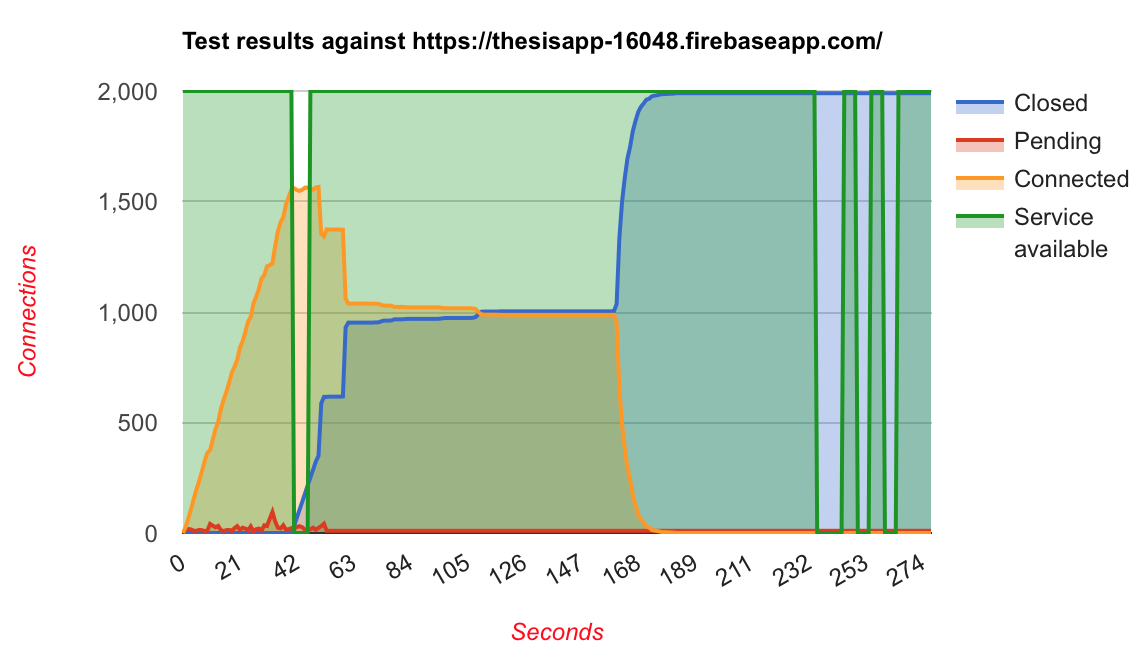
\includegraphics[width=1\textwidth]{ru_dead_yet.png}
  \caption{Apache killer\index{Apache!Killer} attack simulation.}
  \label{fig:ru_dead_yet}
\end{figure}
\subsubsection{Others}
Few other tests have been performed, mostly manual tests. For input fields where human interaction is expected, there exists a bot/automation protection. This includes sending a contact form with a reCAPTCHA\index{reCAPTCHA} check and e-mail confirmation when signing up for a newsletter. When contact form has been sent to the back-end tampering data in HTTP headers\index{Hypertext Transfer Protocol (HTTP)!header} was unsuccessful. A tool called HTTrack Website Copier for copying websites has been used. The website was successfully copied and could be used potentially for phishing\index{Phishing}. However, not all functionalities were rendered correctly causing a lack of application's features which for end users are essential. Thus, it could mitigate certain amount of phishing\index{Phishing} attacks when an attacker would like to use it against a victim.
\subsection{Gray Box Testing}
Limited access to source code helps to investigate security of particular parts of the application. This sometimes cannot be covered by DAST\index{Software!testing!Dynamic Application Security Testing (DAST)} or SAST\index{Software!testing!Static Application Security Testing (SAST)}. Two testing techniques have been found as valuable for this type of security evaluation.
\subsubsection{Cross-Site Request Forgery\index{Cross-Site Request Forgery (CSRF)}}
The most surprising finding is lack of Angular's\index{Angular} protecting against CSRF\index{Cross-Site Request Forgery (CSRF)} without creating custom intercepters. This is an open issue in the official repository of this framework\index{Framework} and has been not solved yet \cite{bib:angular_csrf_issue}. Moreover, discussion across specialized forums gave an insights that to handle this problem the official documentation is missing certain steps \cite{bib:angular_csrf_stackoverflow}. On the other side, following these steps would imply setting \textit{httpOnly} to \textit{false} in cookies, which is not recommended. In such a way cookies\index{Cookies} would be accessible not only for the web server \cite{bib:csurf}. Thus, implementing security against CSRF\index{Cross-Site Request Forgery (CSRF)} would cause lack of security in cookies\index{Cookies} or vice versa. The finding of CSRF has been confirmed by using Acunetix\index{Acunetix} and OWASP ZAP\index{The Open Web Application Security Project (OWASP)!ZAP} web application vulnerabilities scanners.
\subsubsection{File Upload Attack\index{File Upload Attack}}
Files larger than 20 MB are not accepted as upload. However, the front-end\index{Front-end} informs the user that combined files cannot be larger than 20 MB, whilst back-end\index{Back-end} only rejects a single file below 20 MB. For example, uploading a five files, each 19 MB is accepted by the back-end\index{Back-end}. But sending a form with these attachments together was not accepted. These files are still too small to cause DoS\index{Denial of Service (DoS)} from single file upload. Still this could be development improvement. Files different than DOC, DOCX, JPG, JPEG, PDF, PNG, XLS or XLSX are not accepted by both, front-end\index{Front-end} and back-end\index{Back-end}.
\subsubsection{API Keys}
Many secrets are hidden in the environmental variables\index{Environmental Variable}. These includes client-side and server-side API keys\index{Application Programming Interface (API)!key}, credentials and identification data. However, the client side API keys\index{Application Programming Interface (API)!key} are visible in the HTTP headers\index{Hypertext Transfer Protocol (HTTP)!header}. This clearly shows in Figure \ref{fig:recaptcha_api_key}, where the application took the reCAPTCHA\index{reCAPTCHA} API key\index{Application Programming Interface (API)!key} from environmental variables\index{Environmental Variable}. Because of that the only one way to limit access when using client-side API keys\index{Application Programming Interface (API)!key} is to whitelist domains on which it is supposed to be used. The only benefit might be the fact that keeping all API keys\index{Application Programming Interface (API)!key} in one place simplifies management of external services used across the application.
\begin{figure}[ht]
  \centering
      \includegraphics[width=1\textwidth]{recaptcha_api_key.png}
  \caption{HTTP header\index{Hypertext Transfer Protocol (HTTP)!header} with API key\index{Application Programming Interface (API)!key} for reCAPTCHA\index{reCAPTCHA}.}
  \label{fig:recaptcha_api_key}
\end{figure}
\newpage
\subsection{Results}
Based on the validation\index{Validation} results there is no evidence found that the application does not provide a good level of security. Foremost findings are concerns Angular's\index{Angular} SSR\index{Server-Side Rendering (SSR)} design which introduction excludes enabling 100\% security for CSP\index{Content Security Policy (CSP)}. The second unsolved problem is about correct implementation of CSRF\index{Cross-Site Request Forgery (CSRF)}. Furthermore there are some niche findings detected by Skipfish\index{Skipfish} which are difficult to mitigate. Definitely from a network perspective lack of DNSSEC\index{Domain Name System Security Extensions (DNSSEC)} and firewall\index{Firewall} was surprising. Lack of the first one might be due to the reason that the application has been hosted on Firebase domains\index{Firebase!domain} which are not intended for production. In a real scenario it could have been added when owning a domain. The second one should have been added to the Firebase hosting\index{Firebase!hosting}. SAST\index{Software!testing!Static Application Security Testing (SAST)} showed several improvements which could have been done. It looks like these did not influence the results from outside. Findings from the DAST\index{Software!testing!Dynamic Application Security Testing (DAST)} perspective are more about Firebase infrastructure\index{Firebase!infrastructure} and cannot be managed by a developers deploying to that platform. The development mistake with revealing secrets when changing hiding secrets strategy could be critical. It has been fixed on time, but for publicly visible repositories it might be a disaster in some scenarios. Having them in private repositories is not unsafe, but secrets should not be kept there. For this, one of correct solutions is to keep them is in the form of environmental variables\index{Environmental Variable}.
\newpage
\huge Chapter 7
\section{Conclusion}
\normalsize The research project provided lots of valuable information about security in SPAs\index{Single-Page Application (SPA)} based on Angular\index{Angular}. Many techniques have been tested in order to check how to develop an Angular\index{Angular} SPA\index{Single-Page Application (SPA)} in a secure manner. These methods can be divided in two categories: implicitly and explicitly influencing security. Implicitly influencing security is mainly about delivering high quality code, designing robust architecture, implementing tests or programming best practices. Explicitly influencing security is about improving the security itself. The explicit techniques to improve security are related with detecting compilers rules, hiding secrets, limiting access to database, sensitive data and infrastructure, known vulnerabilities\index{Vulnerabilities!Known Vulnerabilities}, requesting manual interaction (e.g. reCAPTCHA\index{reCAPTCHA}), setting up security policies or static code analysis\index{Static Code Analysis}. Implicit factors can influence explicit security. However, in this research the impact has been noticed only slightly due to its medium size. For enterprise projects it can be a more important factor. Projects with an enormous codebase can be very fragile. In these kind of applications, the implicit factors are expected to be more influential on the security itself.\\
\newline
Integrating software security in the SDLC\index{Software Development Life Cycle (SDLC)} of an Angular\index{Angular} application is done in many ways. The continuous security\index{Continuous Security} approach turned out to be crucial for this, where an important element was automation. The methods for different types of testing and security measurements were automated as much as possible, which assisted in catching mistakes or security vulnerabilities\index{Vulnerabilities} much sooner. However, the research showed that not everything can be automated. That is why manual penetration testing with different types of access to source code should be performed.\\
\newline
Many penetration tools have been used to perform a security analysis\index{Security!analysis}. These tools includes Kali Linux\index{Linux!Kali} tools, online scanners and a few others. The results evaluated the security level of the application as good, however it was still doable to find something niche vulnerabilities. It clearly shows that even if most of the tests passes with a very good results with a proper investigation it is doable to find weaknesses. Finding them is one skill, but exploiting them is another. For these kind of sophisticated attacks there is no easy mitigation. The same applies for vulnerabilities\index{Vulnerabilities} which has not yet been reported. There will be always techniques known by small circle of people which can break application. Thus, security can never be fully guaranteed.\\
\newline
Angular\index{Angular} itself provides many built-in protections. However the research showed that the security options which are enabled by the default are not sufficient. Without custom implementation of security defenses such as cookies\index{Cookies} and sessions management, CSP\index{Content Security Policy (CSP)}, security headers\index{Security!header} and CSRF\index{Cross-Site Request Forgery (CSRF)} applications based on Angular should be considered unsecure. The SSR\index{Server-Side Rendering (SSR)} implementation for this framework is far from desired in terms of security. Enforcing by design \textit{unsafe-eval} and \textit{unsafe-inline} effectively weakens carefully implemented CSP\index{Content Security Policy (CSP)}. Mutual exclusion of cookies\index{Cookies} security and protection against CSRF\index{Cross-Site Request Forgery (CSRF)} should be improved as well. Findings by Skipfish\index{Skipfish} showed niche attack vector which are not easy to mitigate. It clearly shows wide spectrum of possible attacks and how difficult is to build security against it. The framework\index{Framework} itself provides a good development environment to develop scalable SPAs\index{Single-Page Application (SPA)}, but for the security part there is still a lot to improve which has been shown in the research.
\clearpage
%TODO: hyperref points to conclusion instead to references.
\addcontentsline{toc}{section}{References}
\begin{thebibliography}{9}
\bibitem{bib:internet_invention}
Tim Berners-Lee, \emph{Information Management: A Proposal}, CERN, Switzerland, March 1989.
\bibitem{bib:preloaded}
Ben Adida, \emph{Helios: Web-based Open-Audit Voting}, Harvard University, 17\textsuperscript{th} USENIX Security Symposium, USENIX Association, pp. 335-348, San Jose, United States, 2008.
\bibitem{bib:owasp_2013}
OWASP, \emph{OWASP Top 10 --- 2013}, The Ten Most Critical Web Application Security Risks, The OWASP Foundation, 2013.
\bibitem{bib:owasp_2017}
OWASP, \emph{OWASP Top 10 --- 2017}, The Ten Most Critical Web Application Security Risks, The OWASP Foundation, 2017.
\bibitem{bib:software_architecture_security}
Mohamed Almorsy, John Grundy, Amani S. Ibrahim, \emph{Automated Software Architecture Security Risk Analysis using Formalized Signatures}, Swinburne University of Technology, ICSE 2013, pp. 662-671, San Francisco, United States, 2013.
\bibitem{bib:software_architecture}
Nenad Medvidovic, Richard N. Taylor, \emph{Software Architecture: Foundations, Theory and Practice}, ICSE'10, pp. 471-472, Cape Town, South Africa, 2010.
\bibitem{bib:ibm_soa}
IBM, \emph{How service-oriented architecture (SOA) impacts your IT infrastructure}, January 2008.
\bibitem{bib:soa_flexibility}
David Sprott, \emph{Business Flexibility Through SOA}, CBDI Forum Limited, 2005.
\bibitem{bib:facebook_data_breach}
Fortune, \emph{Facebook-Cambridge Analytica data breach}, \url{https://www.bbc.com/news/topics/c81zyn0888lt/facebook-cambridge-analytica-data-breach}, last access: 10 January 2019.
\bibitem{bib:marriott_data_breach}
Forbes, \emph{Marriott Breach Exposes Far More Than Just Data}, \url{https://www.forbes.com/sites/davidvolodzko/2018/12/04/marriott-breach-exposes-far-more-than-just-data/}, last access: 10 January 2019.
\bibitem{bib:uber_data_breach}
BBC, \emph{Uber Data Breach Exposed Personal Information of 20 Million Users}, \url{http://fortune.com/2018/04/12/uber-data-breach-security/}, last access: 10 January 2019.
\bibitem{bib:cryptocurrencies_hacking}
Techopedia, \emph{Hacking Activities Increase Along with Cryptocurrency Pricing}, \url{https://www.techopedia.com/hacking-activities-increase-along-with-cryptocurrency-pricing/2/33174}, last access: 10 January 2019.
\bibitem{bib:gdpr_eu}
European Parliament and of the Council, \emph{Regulation (EU) 2016/679}, Official Journal of the European Union, April 2016.
\bibitem{bib:cyber_security_incidents}
Varonis, \emph{60 Must-Know Cybersecurity Statistics for 2019}, \url{https://www.varonis.com/blog/cybersecurity-statistics/}, last access: 10 January 2019.
\bibitem{bib:building_security_in}
Gary R. McGraw, \emph{Building Security In}, Addison-Wesley, 2006.
\bibitem{bib:soap_api}
PayPal, \emph{PayPal SOAP API Basics}, \url{https://developer.paypal.com/docs/classic/api/PayPalSOAPAPIArchitecture/}, last access: 14 January 2019.
\bibitem{bib:wordpress_api}
WordPress, \emph{REST API Handbook}, \url{https://developer.wordpress.org/rest-api/}, last access: 14 January 2019.
\bibitem{bib:parsing}
Microsoft, \emph{JSON parsing 10x faster than XML parsing}, \url{https://blogs.msdn.microsoft.com/sqlserverstorageengine/2017/11/13/json-parsing-10x-faster-than-xml-parsing/}, last access: 3 June 2019.
\bibitem{bib:owasp_rest_security}
OWASP, \emph{REST Security Cheat Sheet}, \url{https://www.owasp.org/index.php/REST_Security_Cheat_Sheet}, last access: 14 January 2019.
\bibitem{bib:vulnerability_fsecure}
F-Secure Labs, \emph{Vulnerabilities}, \url{https://www.f-secure.com/en/web/labs_global/vulnerabilities}, last access: 31 January 2019.
\bibitem{bib:cloud_vulnerabilities}
Bernd Grobauer, Elmar Stöcker, Tobias Walloschek, \emph{Understanding Cloud Computing Vulnerabilities}, Siemens, IEEE Security \& Privacy, pp. 50-57, March-April 2011.
\bibitem{bib:nist_list}
NIST, \emph{National Vulnerability Database}, \url{https://nvd.nist.gov/vuln}, last access: 17 January 2019.
\bibitem{bib:cve_website}
CVE, \emph{Publicly known Cybersecurity Vulnerabilities}, \url{https://cve.mitre.org/index.html}, last access: 17 January 2019.
\bibitem{bib:thomas}
Thomas S. Beekman, \emph{Auditing Information Security in Mobile Device-enabled Infrastructure}, Erasmus School of Accounting \& Assurance Rotterdam, Leiderdorp, Netherlands, 3 October 2016.
\bibitem{bib:owasp_controls}
OWASP, \emph{OWASP Proactive Controls}, \url{https://www.owasp.org/index.php/OWASP_Proactive_Controls#tab=OWASP_Proactive_Controls_2016}, last access: 10 January 2019.
\bibitem{bib:stack_overflow_report}
Stack Overflow, \emph{Developer Survey Results 2018}, \url{https://insights.stackoverflow.com/survey/2018#most-popular-technologies?utm_source=codecademyblog}, last access: 18 January 2018.
\bibitem{bib:csp_reference}
Foundeo Inc., \emph{Content Security Policy Reference}, \url{https://content-security-policy.com/}, last access: 8 January 2019.
\bibitem{bib:csp_google}
Google Developers, \emph{Content Security Policy}, \url{https://developers.google.com/web/fundamentals/security/csp/}, last access: 8 January 2019.
\bibitem{bib:owasp_csrf}
OWASP, \emph{Cross-Site Request Forgery (CSRF)}, \url{https://www.owasp.org/index.php/Cross-Site_Request_Forgery_(CSRF)}, last access: 8 January 2019.
\bibitem{bib:owasp_prevention}
OWASP, \emph{Cross-Site Request Forgery (CSRF) Prevention Cheat Sheet}, \url{https://www.owasp.org/index.php/Cross-Site_Request_Forgery_(CSRF)_Prevention_Cheat_Sheet}, last access: 8 January 2019.
\bibitem{bib:robust_defenses}
Adam Barth, Collin Jackson, John C. Mitchell, \emph{Robust Defenses for Cross-Site Request Forgery}, Stanford University, Alexandria, United States, 2008.
\bibitem{bib:angular_security}
Google, \emph{Angular --- Security}, \url{https://angular.io/guide/security}, last access: 9 January 2019.
\bibitem{bib:caniuse_cors}
Can I use..., \emph{Cross-Origin Resource Sharing}, \url{https://caniuse.com/#search=cors}, last access: 20 February 2019.
\bibitem{bib:js_best_practices}
W3Schools, \emph{JavaScript Best Practices}, \url{https://www.w3schools.com/js/js_best_practices.asp}, Refsnes Data, last access: 20 December 2018.
\bibitem{bib:ts_best_practices}
Microsoft, \emph{Do's and Don'ts}, \url{https://www.typescriptlang.org/docs/handbook/declaration-files/do-s-and-don-ts.html}, last access: 21 December 2018.
\bibitem{bib:angular_best_practices}
Google, \emph{Angular --- Style Guide}, \url{https://angular.io/guide/styleguide}, last access: 22 December 2018.
\bibitem{bib:general_best_practices}
Envato Tuts+, \emph{Top 15+ Best Practices for Writing Super Readable Code}, \url{https://code.tutsplus.com/tutorials/top-15-best-practices-for-writing-super-readable-code--net-8118}, last access: 20 February 2019.
\bibitem{bib:modularity}
Yuanfang Cai, Ben Hallen, William G. Griswold, Kevin J. Sullivan, \emph{The Structure and Value of Modularity in Software Design}, ACM 2001, pp. 99-108, Vienna, Austria, September 2001.
\bibitem{bib:modules_standard}
Standard ECMA-262, \emph{ECMAScript 2015 Language Specification}, Sections: 15.2.2 Imports and 15.2.3 Exports, Ecma International, Geneva, Switzerland, June 2015.
\bibitem{bib:typescript_compiler_settings}
Microsoft, \emph{Compiler Options TypeScript}, \url{https://www.typescriptlang.org/docs/handbook/compiler-options.html}, last access: 5 March 2019.
\bibitem{bib:modules_comparison}
Auth0, \emph{JavaScript Module Systems Showdown: CommonJS vs AMD vs ES2015}, \url{https://auth0.com/blog/javascript-module-systems-showdown/}, last access: 29 May 2019.
\bibitem{bib:angular_states}
Victor Savkin, \emph{Managing State in Angular Applications}, \url{https://blog.nrwl.io/managing-state-in-angular-applications-22b75ef5625f}, last access: 8 August 2019.
\bibitem{bib:npm_incident}
The npm Blog, \emph{Details about the event-stream incident}, \url{https://blog.npmjs.org/post/180565383195/details-about-the-event-stream-incident}, last access: 17 January 2019.
\bibitem{bib:stealing_envvar}
BleepingComputer.com, \emph{JavaScript Packages Caught Stealing Environment Variables}, \url{https://www.bleepingcomputer.com/news/security/javascript-packages-caught-stealing-environment-variables/}, last access: 31 May 2019.
\bibitem{bib:eslint}
ESLint, \emph{Postmortem for Malicious Packages Published on July 12th, 2018}, \url{https://eslint.org/blog/2018/07/postmortem-for-malicious-package-publishes}, last access: 31 May 2019.
\bibitem{bib:getcookies}
The npm Blog, \emph{Reported malicious module: getcookies}, \url{https://blog.npmjs.org/post/173526807575/reported-malicious-module-getcookies}, last access: 31 May 2019.
\bibitem{bib:docker_container}
Jurgen Cito, Harald C. Gall, Philipp Leitner, Gerald Schermann, John Erik Wittern, Sali Zumberi, \emph{An Empirical Analysis of the
Docker Container Ecosystem on GitHub}, 2017 IEEE/ACM 14\textsuperscript{th} International Conference on Mining Software Repositories (MSR), pp. 323-333, Buenos Aires, Argentina, 20-21 May 2017.
\bibitem{bib:containers_features}
Emily Freeman, \emph{DevOps For Dummies}, John Wiley \& Sons Inc., 2019.
\bibitem{bib:software_security_testing}
Gary McGraw, Bruce Potter, \emph{Software Security Testing}, IEEE Security \& Privacy, pp. 81-85, September-October 2004.
\bibitem{bib:dast_vs_sast}
Synopsys, \emph{SAST vs. DAST: What’s the best method for application security testing?}, \url{https://www.synopsys.com/blogs/software-security/sast-vs-dast-difference/}, last access: 8 August 2019.
\bibitem{bib:framework_for_scrum}
Ihab Mohamed Abdelwahab, Nagy Ramadan Darwish, \emph{A Security Testing Framework for Scrum based Projects}, IJCA, pp. 12-17, March 2016.
\bibitem{bib:pentesting_in_agile}
Tomas Klima, Martin Tomanek, \emph{Penetration Testing in Agile Software Development Projects}, IJCIS, pp. 1-7, March 2015.
\bibitem{bib:cde_challenges}
Lianping Chen, \emph{Continuous delivery: Huge benefits, but challenges too}, IEEE Software, pp. 50-54, March/April 2015.
\bibitem{bib:cd_facebook}
Kent Beck, Mitchell Douglas, Michael Gentili, Tony Savor, Michael Stumm, Laurie Williams, \emph{Continuous Deployment at Facebook and OANDA}, ICSE'16 Companion, pp. 21-30, Austin, United States, 14-22 May 2016.
\bibitem{bib:ci_cd_all}
Muhammad Ali Babara, Mojtaba Shahina, Liming Zhub, \emph{Continuous Integration, Delivery and Deployment: A Systematic Review on Approaches, Tools, Challenges and Practices}, IEEE, pp. 1-32, 2016.
\bibitem{bib:security_cde}
Muhammad Ali Babar, Adam Johannes Raf, Mojtaba Shahin, Faheem Ullah, Mansooreh Zahedi, \emph{Security Support in Continuous Deployment Pipeline}, 2017.
\bibitem{bib:gwt_approach}
Robert C. Martin, \emph{The Truth about BDD}, \url{https://sites.google.com/site/unclebobconsultingllc/the-truth-about-bdd}, last access: 8 August 2019.
\bibitem{bib:secure_architecture}
Eduardo Fernandez-Buglioni, \emph{Security Patterns in Practice: Designing Secure Architectures Using Software Patterns}, John Wiley \& Sons Inc., 2013.
\bibitem{bib:wai_aria}
World Wide Web Consortium, \emph{Accessible Rich Internet Applications (WAI-ARIA) 1.1}, W3C Recommendation, December 2017.
\bibitem{bib:angular_browser_support}
Google, \emph{Angular --- Browser support}, \url{https://angular.io/guide/browser-support}, last access: 4 March 2019.
\bibitem{bib:expect-ct}
Threatpost, \emph{Google to Ditch Public Key Pinning in Chrome}, \url{https://threatpost.com/google-to-ditch-public-key-pinning-in-chrome/128679/}, last access: 8 August 2019.
\bibitem{bib:cleancode}
Robert C. Martin, \emph{Clean Code: A Handbook of Agile Software Craftsmanship}, Prentice Hall, 2009.
\bibitem{bib:cwe_variables}
Common Weakness Enumeration, \emph{CWE-457: Use of Uninitialized Variable}, \url{https://cwe.mitre.org/data/definitions/457.html}, last access: 19 August 2019.
\bibitem{bib:type_study}
Earl T. Barr, Christian Bird, Zheng Gao, \emph{To Type or Not to Type: Quantifying Detectable Bugs in JavaScript}, IEEE, 2017.
\bibitem{bib:riteway}
Eric Elliott, \emph{RITEway}, \url{https://github.com/ericelliott/riteway}, last access: 12 March 2019.
\bibitem{bib:efficient_code_coverage}
Yong Woo Kim, \emph{Efficient use of code coverage in large-scale software development}, CASCON '03, pp. 145-155, Toronto, Canada, 6-9 October 2003.
\bibitem{bib:unit_test_questions}
Eric Elliott, \emph{5 Questions Every Unit Test Must Answer}, \url{https://medium.com/javascript-scene/what-every-unit-test-needs-f6cd34d9836d}, last access: 12 March 2019.
\bibitem{bib:ssr_vs_csr}
Alex Grigoryan, \emph{The Benefits of Server Side Rendering Over Client Side Rendering}, \url{https://medium.com/walmartlabs/the-benefits-of-server-side-rendering-over-client-side-rendering-5d07ff2cefe8}, last access: 26 August 2019.
\bibitem{bib:es5_browser_support}
Kangax, \emph{ECMAScript 5 compatibility table}, \url{http://kangax.github.io/compat-table/es5/}, last access: 4 March 2019.
\bibitem{bib:semver}
OSGi Alliance, \emph{Semantic Versioning}, 6 May 2010.
\bibitem{bib:angular_coverage}
Jared Youtsey, \emph{Angular Unit Testing Code-Coverage Lies}, \url{https://medium.com/ngconf/angular-unit-testing-code-coverage-lies-603c6c85f801}, last access: 29 August 2019.
\bibitem{bib:ssl_compatibility}
Mozilla, \emph{Security/Server Side TLS}, \url{https://wiki.mozilla.org/Security/Server_Side_TLS}, last access: 29 August 2019.
\bibitem{bib:nmap_documentation}
Nmap: the Network Mapper - Free Security Scanner, \emph{Usage and Examples}, \url{https://nmap.org/book/osdetect-usage.html}, last access: 29 August 2019.
\bibitem{bib:nmap_source_code}
Nmap: the Network Mapper - Free Security Scanner, \emph{GitHub source code repository}, \url{https://github.com/nmap/nmap/blob/ac2e140a1483f2c539e71c1aba354d31c8952fc4/osscan2.cc#L410}, last access: 29 August 2019.
\bibitem{bib:angular_csrf_issue}
Angular - GitHub, \emph{GitHub source code repository open issue: HttpClient does not set X-XSRF-Token on Http Post}, \url{https://github.com/angular/angular/issues/20511}, last access: 29 August 2019.
\bibitem{bib:angular_csrf_stackoverflow}
Stack Overflow, \emph{Angular 6 does not add X-XSRF-TOKEN header to http request}, \url{https://stackoverflow.com/questions/50510998/angular-6-does-not-add-x-xsrf-token-header-to-http-request/50511663}, last access: 29 August 2019.
\bibitem{bib:csurf}
CSRF token middleware, \emph{GitHub source code repository: cookie documentation}, \url{https://github.com/expressjs/csurf#cookie}, last access: 29 August 2019. 
\end{thebibliography}
\newpage
\appendix
\addcontentsline{toc}{section}{Appendices}
\section*{Appendices}
\section{UI Design Elements}
\label{sec:appendices}
\begin{figure}[ht]
  \centering
      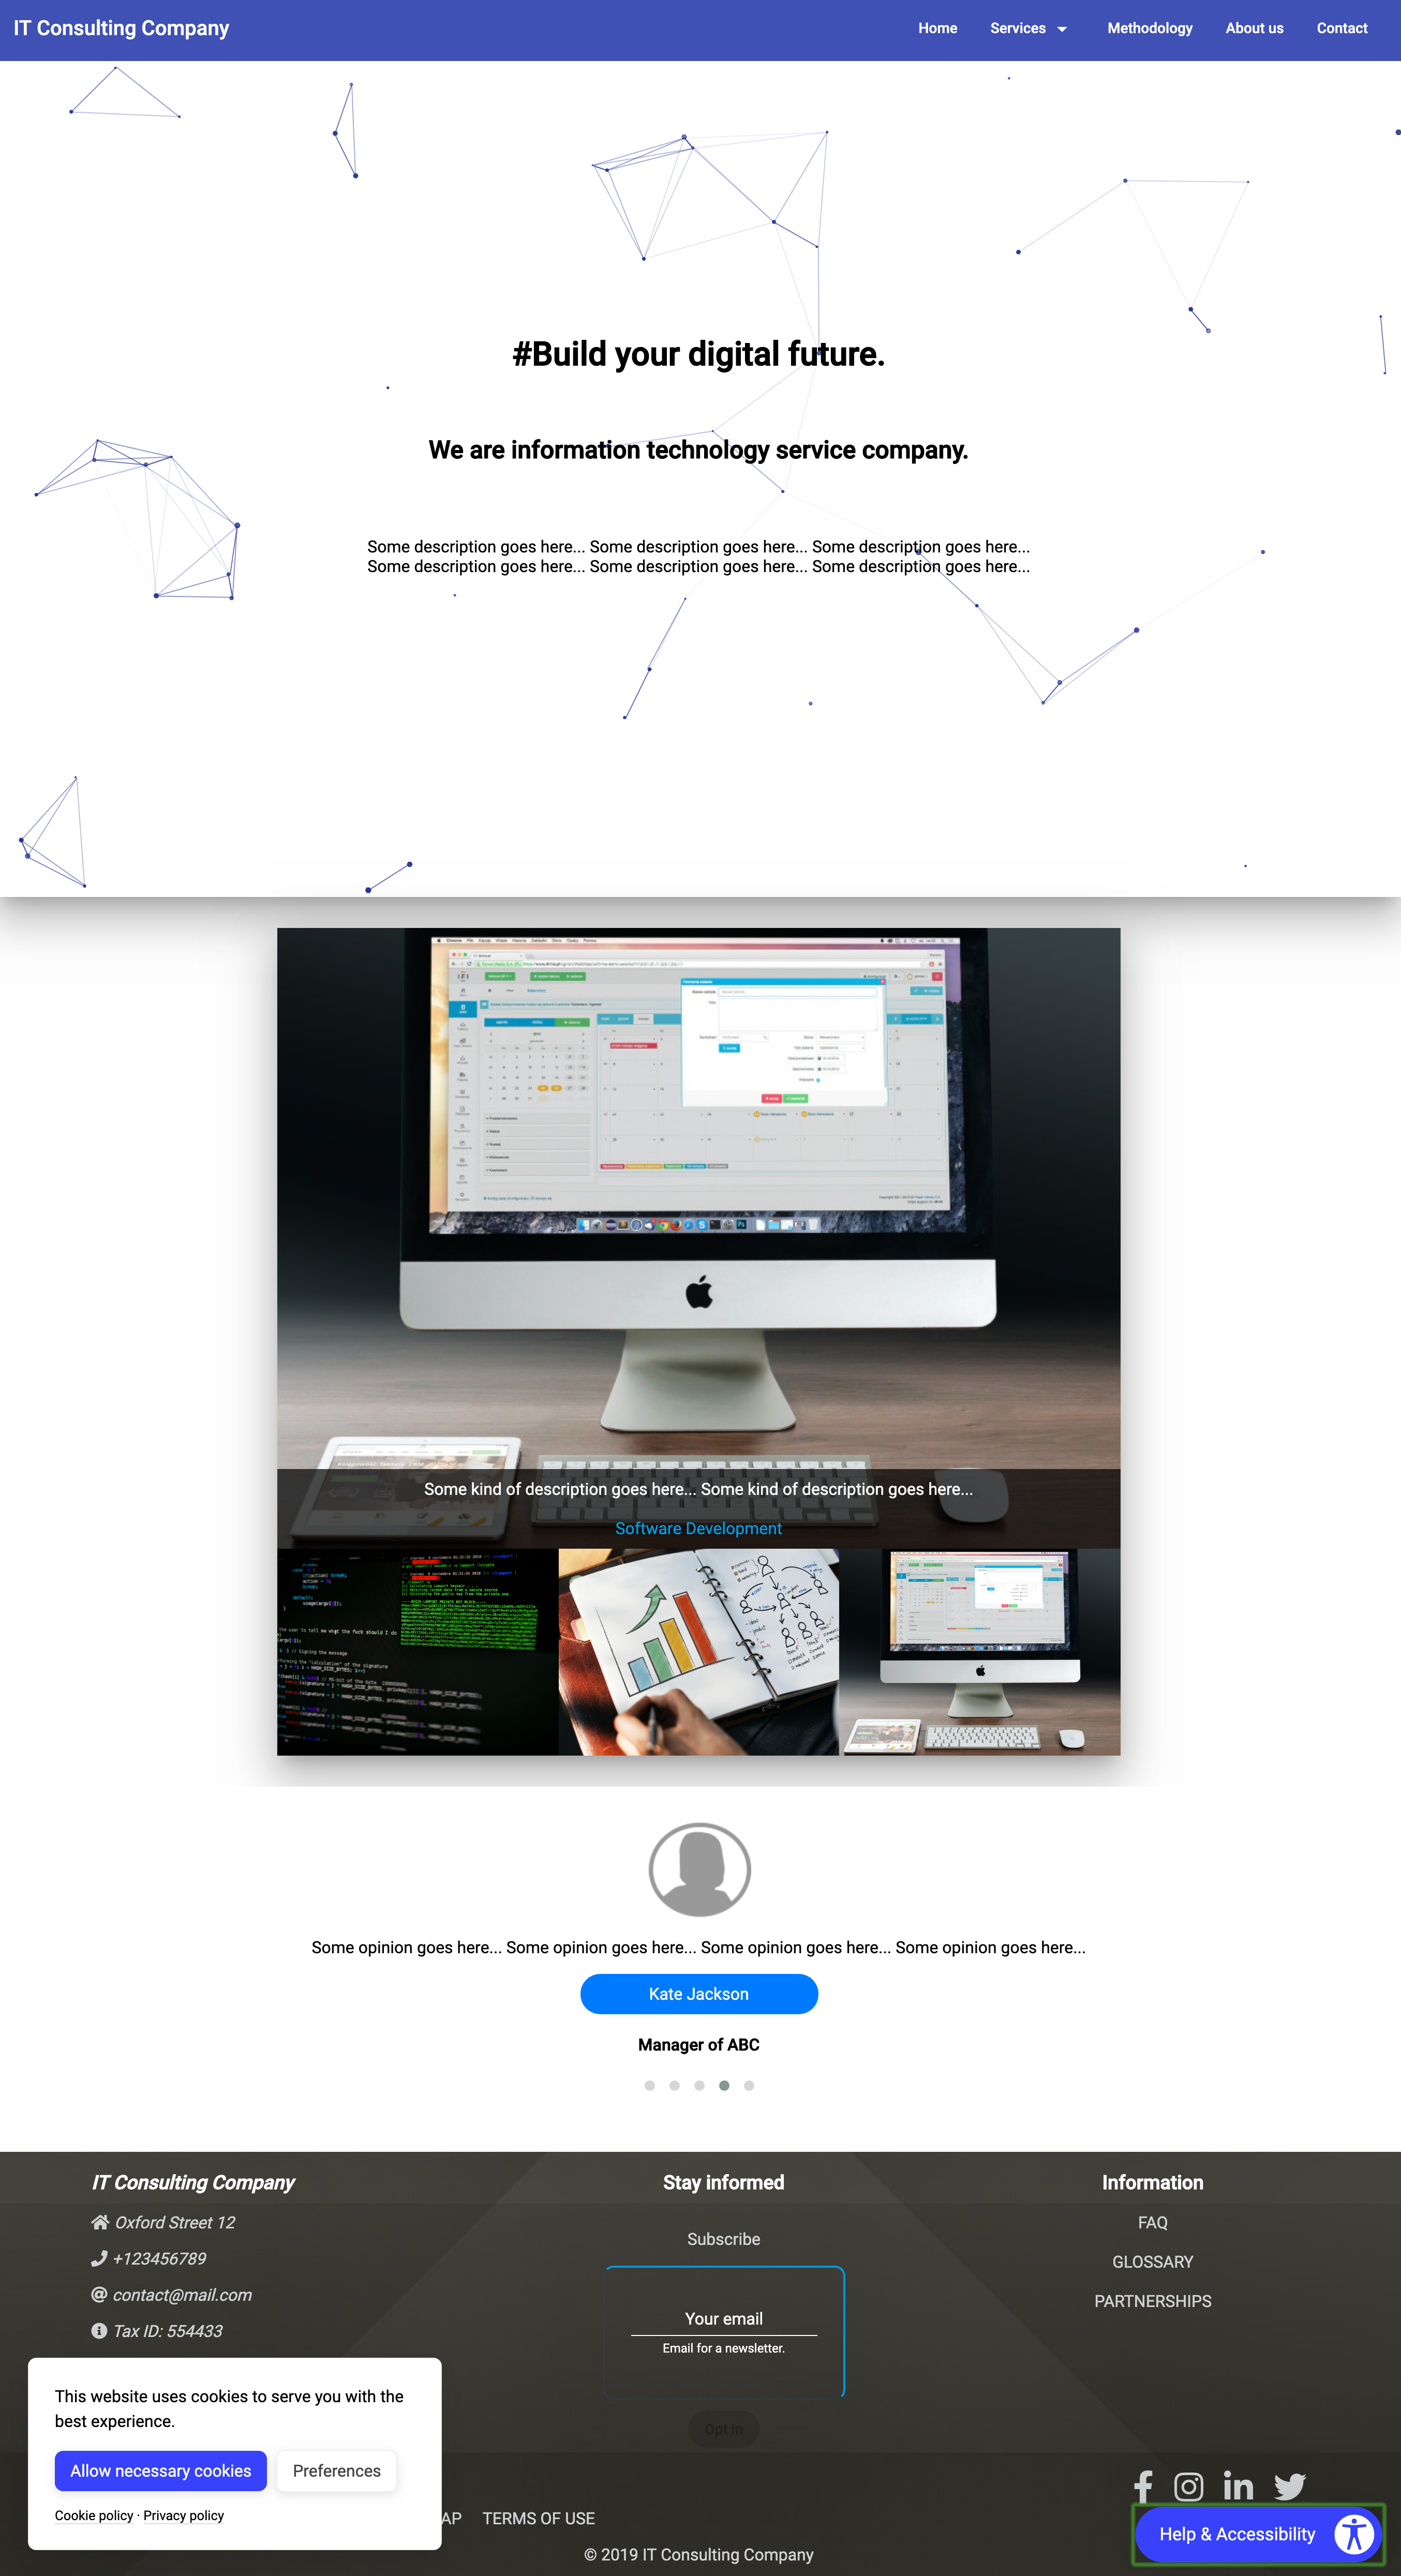
\includegraphics[width=0.6\textwidth]{thesisapp1.png}
\end{figure}
\begin{figure}[ht]
  \centering
      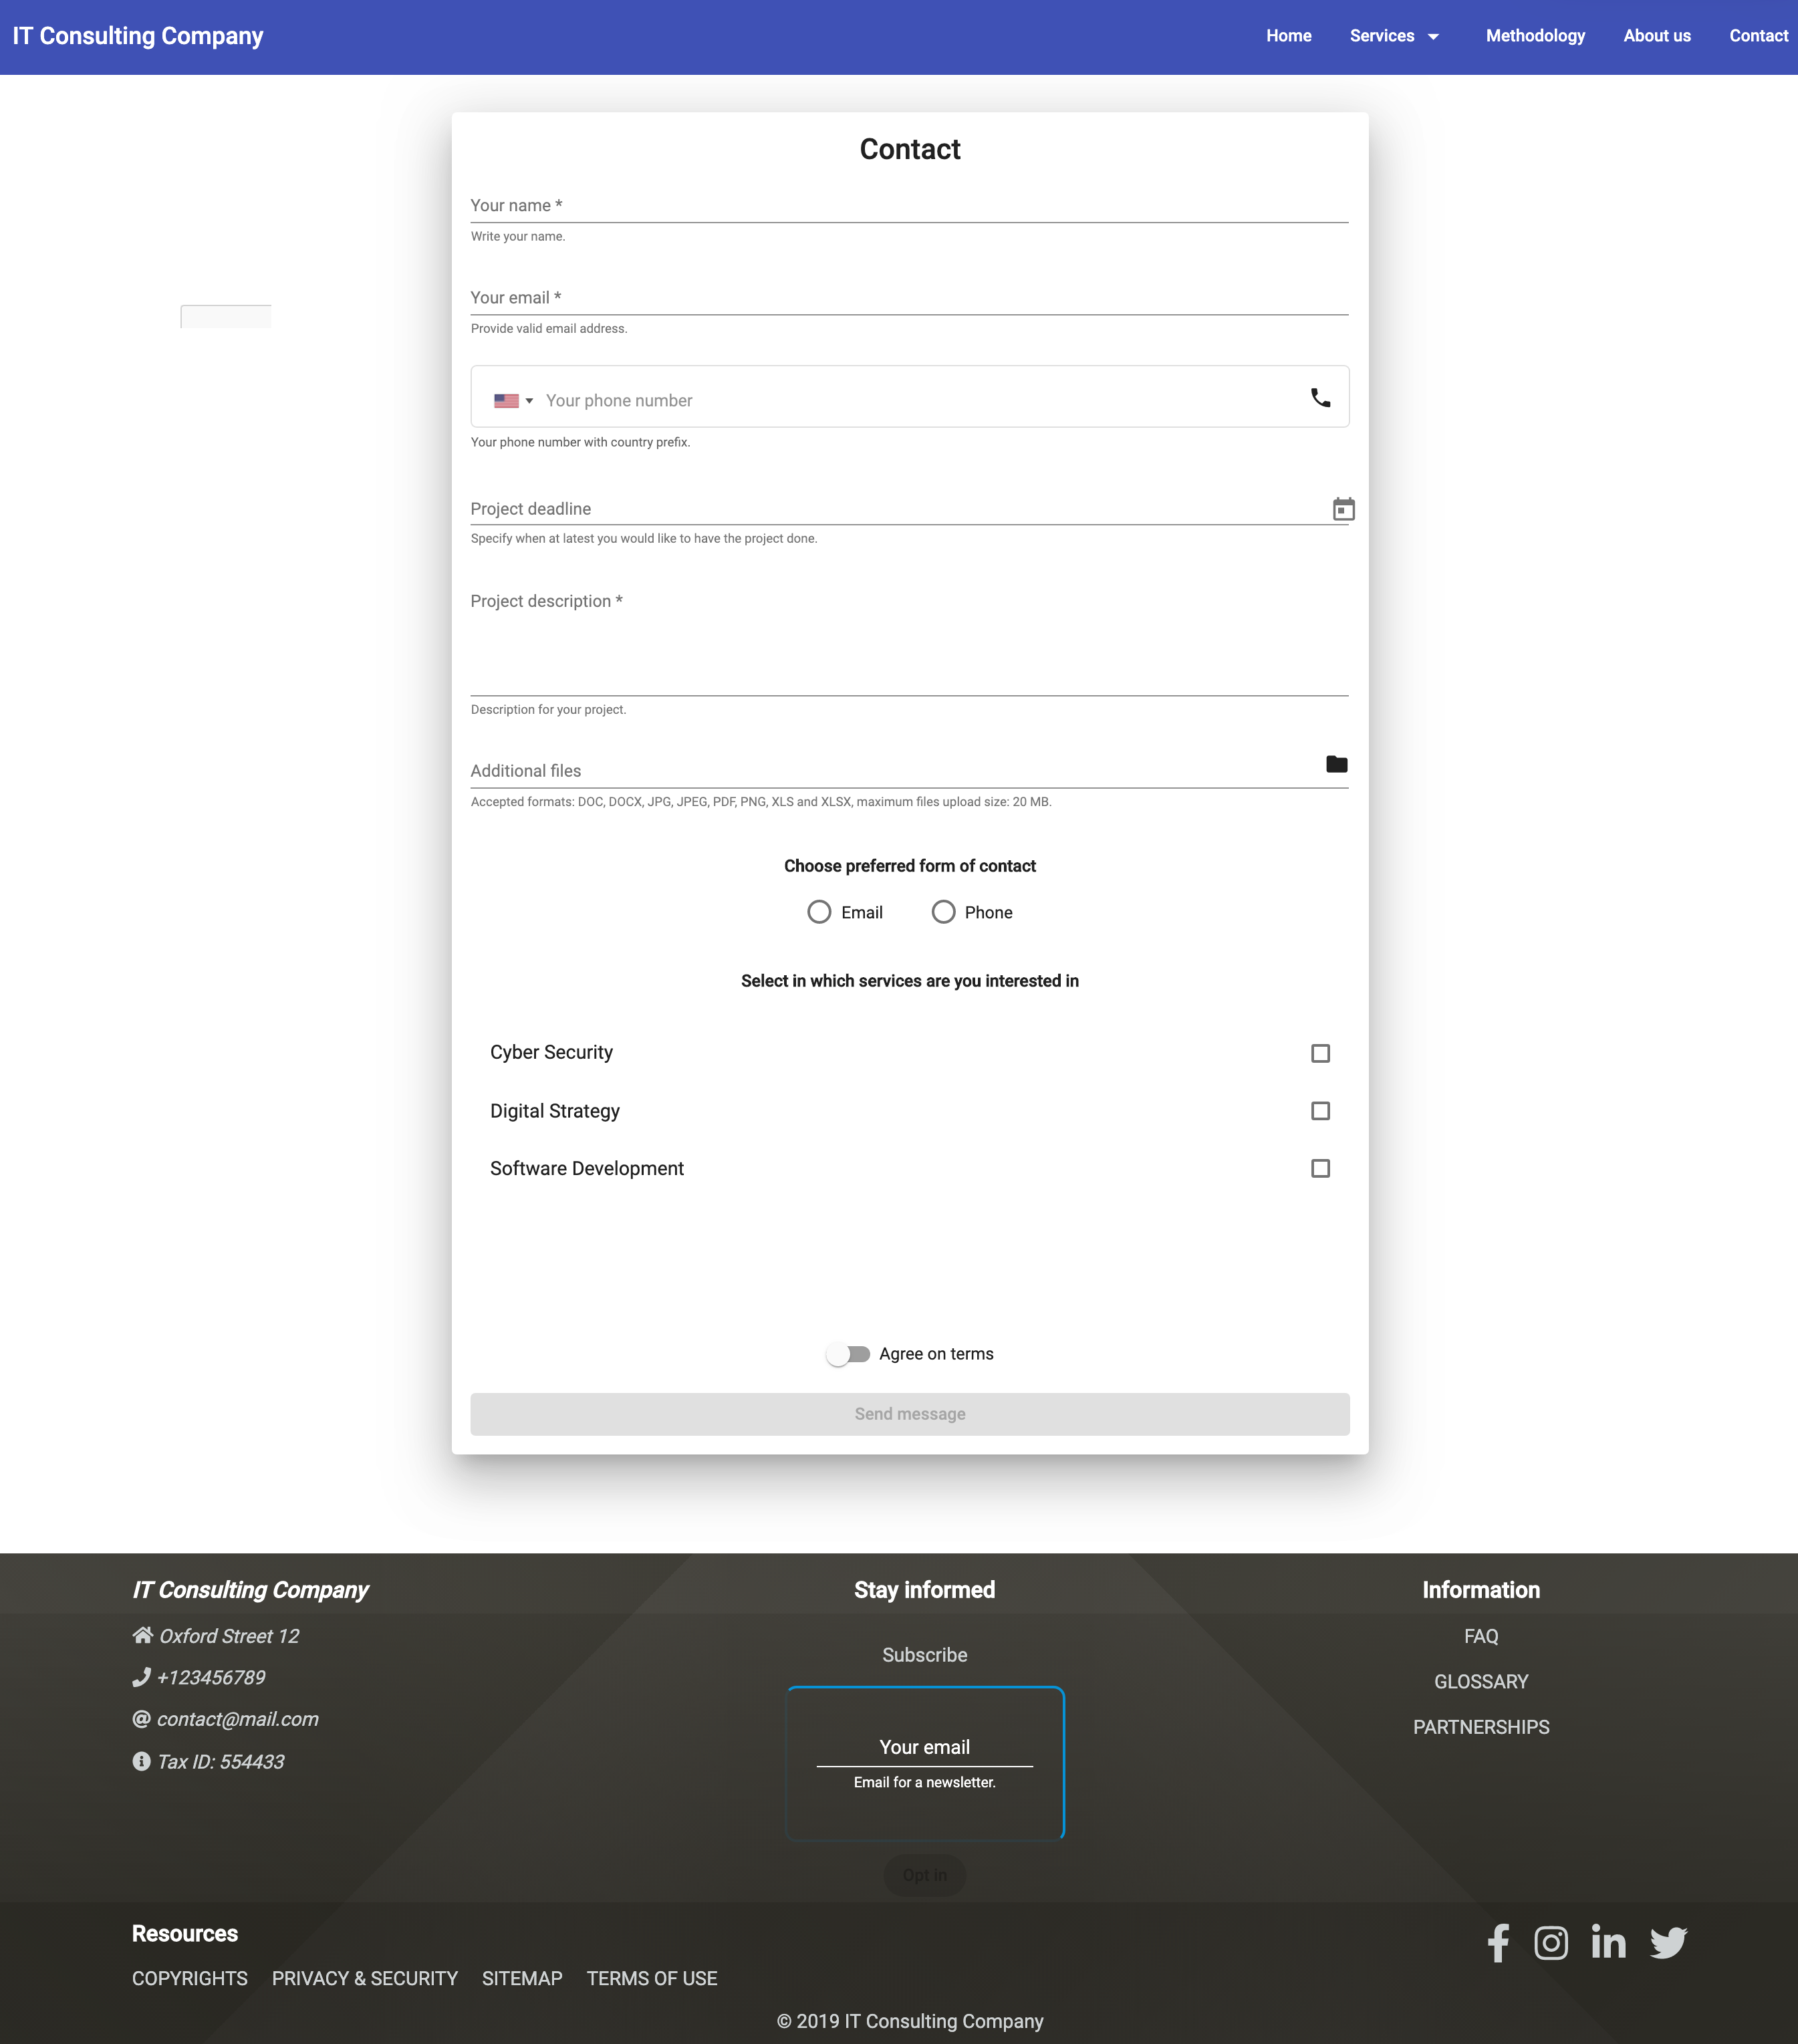
\includegraphics[width=1\textwidth]{thesisapp2.png}
\end{figure}
\begin{figure}[ht]
  \centering
      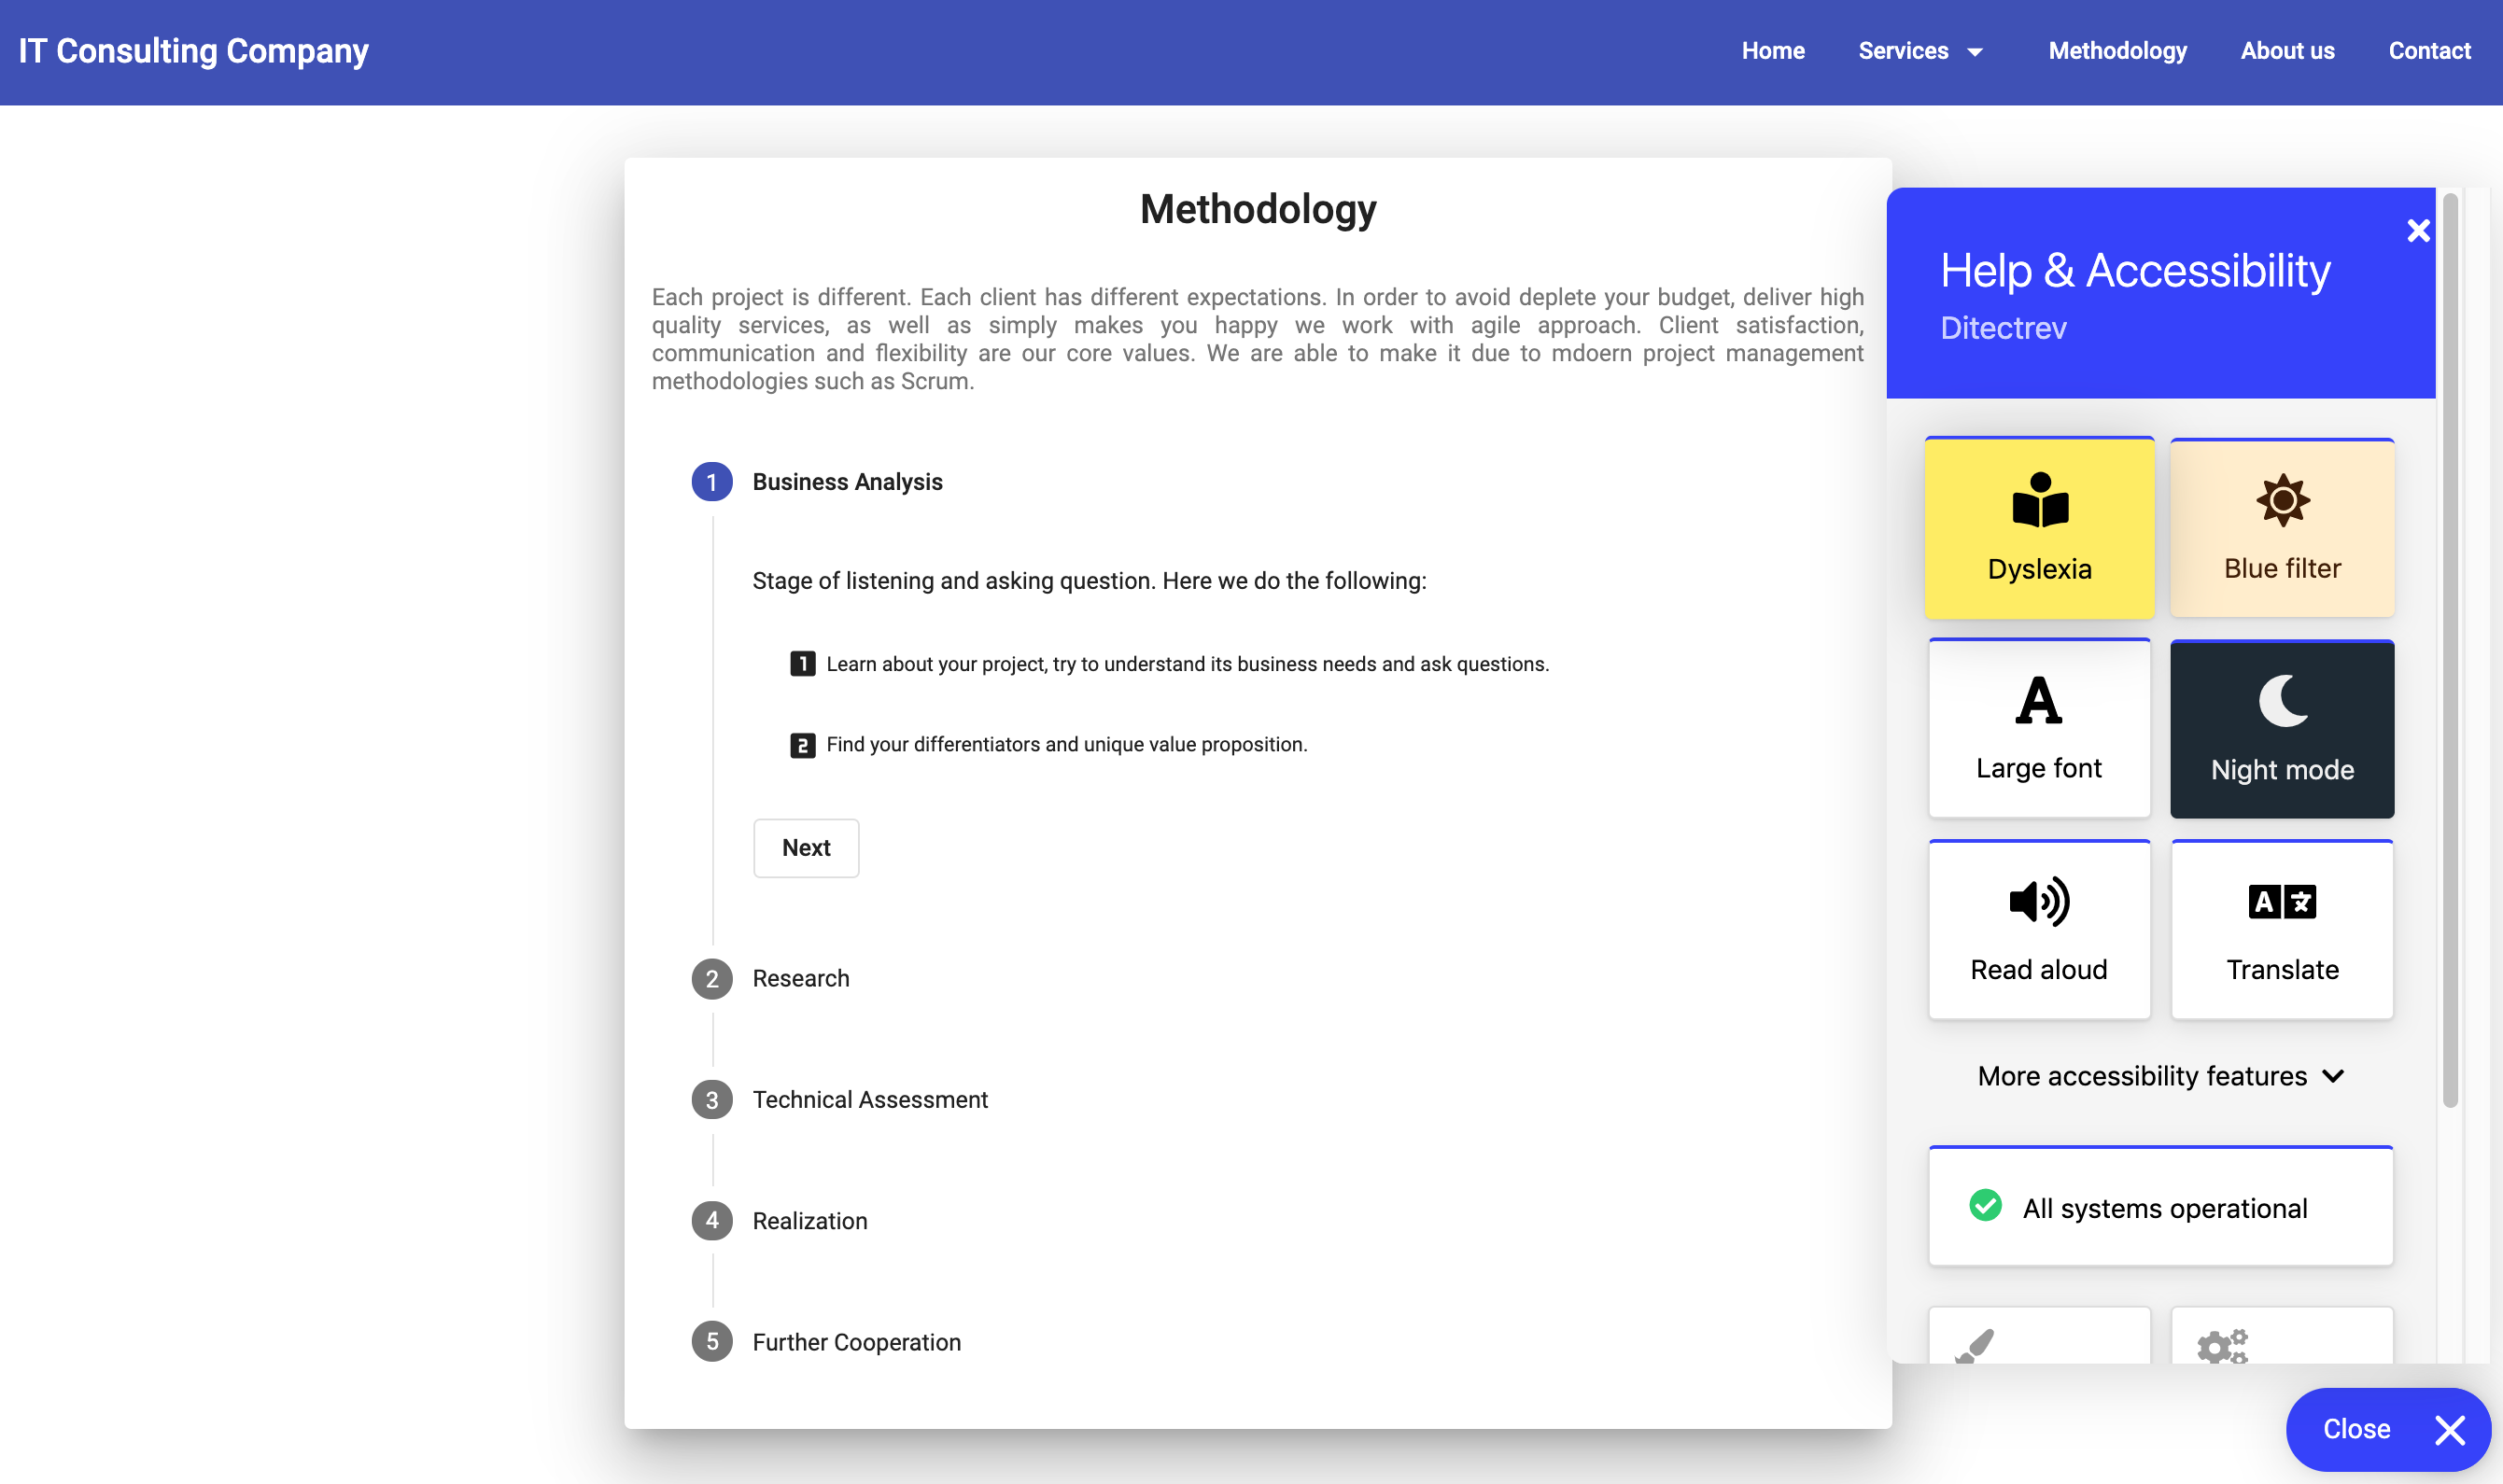
\includegraphics[width=1\textwidth]{thesisapp3.png}
\end{figure}
\begin{figure}[ht]
  \centering
      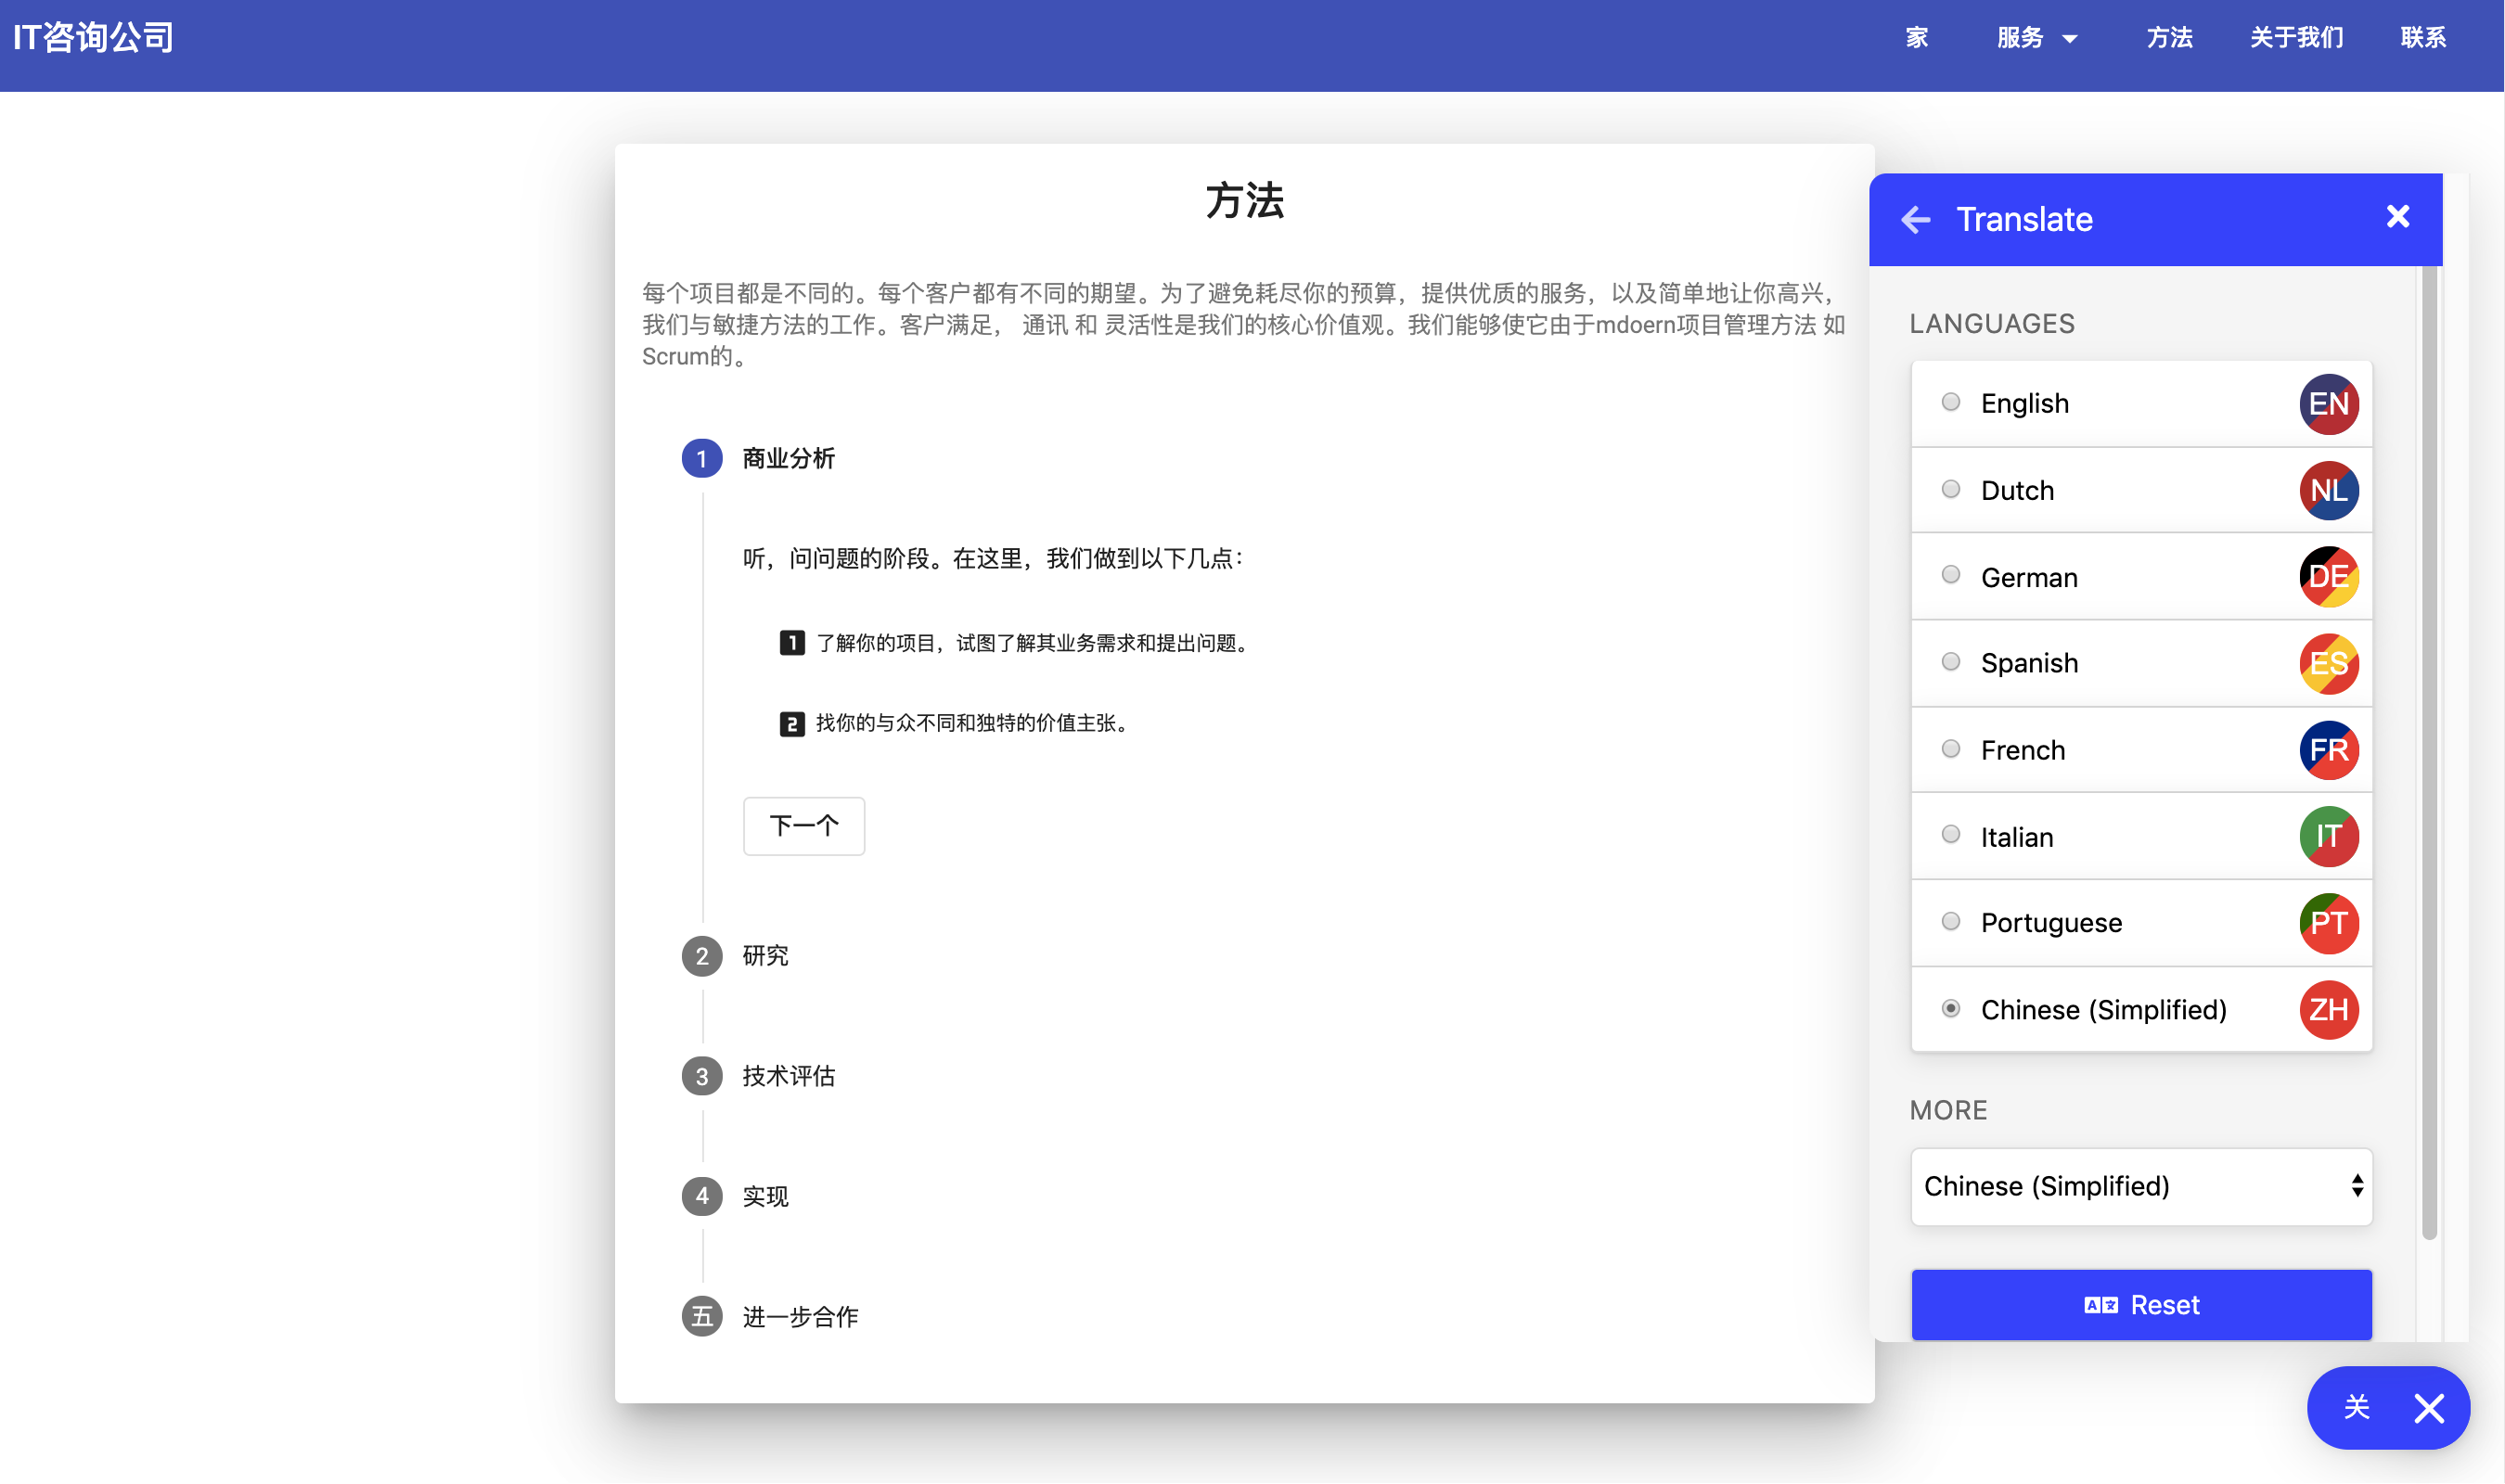
\includegraphics[width=1\textwidth]{thesisapp4.png}
\end{figure}
\printindex
\end{document}